\chapter{The wildfire-habitat connectivity dilemma: a graph theoretical approach to landscape management}
\label{chapter2}
\begin{center}
	\begin{minipage}{.9\textwidth}
This article is co-authored with L. Mouysset and under review at 
	\end{minipage}
    \vspace*{.2cm}
    
\textbf{Abstract}\par
    \vspace*{.2cm}
    \noindent
    \begin{minipage}{0.9\textwidth}
	\singlespacing
\textbf{Background:} Fuel treatment operations help to mitigate the spread and severity of wildfires in numerous ecosystems. As they aim at fragmenting the fire landscape, they also fragment wildlife posing a dilemma for land managers. We use graph theory on simulated to gain a general understanding of the allocation of treatments over space and time and the corresponding landscape properties with various habitat connectivity targets. 
 
\textbf{Results:} Our results show that all initial landscapes converge to steady-state landscape cycles. Optimal trajectories significantly reduce wildfire risk while safeguarding habitat connectivity. As the policy budget increases, more risk reduction is achieved, albeit with a decreasing marginal efficiency. As habitat targets increase, increasing the budget is of no effect, and risk increases. Landscapes are less risky, more fragmented, and diverse when the budget is large and biodiversity targets are low, while they are more compact and less diverse when the opposite is true. Treatment allocation follows graph centrality measures, and central cells are treated first. When biodiversity targets increase, central cells are no longer treated as they decrease habitat connectivity. Treatment is reshuffled to the edges of the landscape.


\textbf{Conclusion:} Computational experiments generalize existing results. Using graph theory, general insights can be gained, and help managers faced with multiple objectives in forested landscapes. From a policy perspective, in the face of climate change, increasing treatment budgets should be a priority to avoid increasing damages. A key guideline is treating \textit{adolescent} successional stages and fragment \textit{mature} patches to mitigate risk and guarantee the connectivity of wildlife habitat. 
\\\\
\textbf{Keywords : }Fuel treatment, connectivity, wildfire risk, wildlife habitat, spatial optimization, graph theory
\end{minipage}
\end{center}

\vfill
\newpage
%%% Manuscript


\begin{itemize}
\item We have a problem at extending
\item Edge effects
\item Difficulty to extend the critical node detection problem with no special structure graphs
\item Betweenness centrality is not enough
\end{itemize}
Solution : get rid of the large scale and focus on the small scale, and say future research avenues involve understanding the transitional path.
\newpage


\section{Introduction}
% Motivation : why should we care about wildfires? 
\hspace*{1.5em}Hazardous and intense wildfires destroy forest cover\footnote{From 2001 to 2023, forest loss attributed to wildfires amounted to 138 million hectares (roughly 33\% of the surface of the European Union) \citep{tyukavina_global_2022}}, threaten forest resilience and can cause ecosystem shifts, ranging from changes in forest structure to changes towards non-forest ecosystems \citep{coop_wildfire-driven_2020}. 
Additionally, intense wildfires cause human damages, in the form of direct asset losses: in 2018, wildfires in California have caused \$ 27 billion \citep{wang_economic_2021}. Indirect costs are also of concern, especially related to wildfire smoke : increases in PM 2.5 concentrations have important health impacts \citep{burke_wildfire_2023, heft-neal_behavior_2023}, smoke directly affects recreation values in the US, amounting to \$USD 2.3 billion in welfare losses \citep{Gellman}. Aside from directly measurable costs, wildfires also cause dramatic impacts on biodiversity across taxa \citep{Wintle2020}, through direct population losses and durable habitat disruption \citep{Ayars2023}.
%
\\
\hspace*{1.5em}In a business as usual scenario in terms of forest management, wildland-urban interface expansion and climate change, these direct and indirect costs and damages to both humans and non-humans are expected to increase drastically.
%
\\
Decades of wildfire suppression have created a ``wildfire deficit'', which increases the probability, extent and severity of wildfires in the western United States \citep{kreider_fire_2024}. European forests are not adapted to climate change induced wildfire risks \citep{Khabarov2014ForestFA}, in terms of species composition and use of fuel management operations. Mechanical thinning, prescribed burns, and sometimes, logging, have been leveraged to decrease the fuel load in risky areas and theoretically decrease the probability and severity of burns upon wildfire occurence\footnote{The efficiency of these measures depends on environmental and terrain variables. For example, prescribed burns are efficient every 1-4 years in reducing risk and severity only in the case of non-extreme weather conditions, and when the terrain ruggedness is limited \citep{bradstock_1998}}. In numerous regions, such as conifer forests in California \citep{Vaillant2009, Kalies2016, low_shaded_2023}, eucalypt forests in South Western Australia \citep{burrows2013, boer_long-term_2009, Florec2020}, southern Europe \citep{Fernandes2013}, evidence shows that fuel treatments, can mitigate wildfire intensity and spread. Land management agencies have historically implemented these policies in Australia \citep{burrows2013}, Europe, and the United States (and are projected to ramp up, for example under the Infrastructure Investment and Jobs Act of 2021 in the US). While potentially useful, the use of these treatments is still hindered by numerous obstacles \citep{miller_barriers_2020} and remains insufficient\footnote{ However, recent bills have been passed in the US (Infrastructure Investment and Jobs Act of 2021) and California to ramp up the use of prescribed burns - such as \href{https://wildfiretaskforce.org/about/expenditure-plan/}{the bugdget act of 2022}, committing \$2.8 billion to the Governor’s Wildfire and Forest Resilience Action Plan - and limiting liabilities in the case of wildfire escape (see \href{https://openstates.org/ca/bills/20212022/SB332/}{California Senate Bill SB-332}) on private land.}. 
Additionally, the extension of wildland-urban interfaces (WUI) increases the extent of potential damages as well as ignition probabilities \citep{radeloff_rapid_2018}.
\\
As global warming affects water supply and fuel moisture \citep{jolly_climate-induced_2015, Abatzoglou, ruffault_extreme_2018}, it is projected to increase the frequency, severity, and magnitude of wildfires \citep{Dupuy2019ClimateCI, wasserman_climate_2023}. Recent wildfire events in California (since 2018), in Australia (2019-2020), and in Europe (France, Portugal, Greece in 2022) have epitomized these trends. 
%
Moreover, wildfires and climate change are endogeneously linked in a positive feedback loop : large wildfires are of importance in the face of climate change; as they release large amounts of greenhouse gases ($1.7GtC$ per year on average between 2003 and 2022) and reduce the extent of terrestrial carbon sinks \citep{zheng_record-high_2023, friedlingstein_2023, byrne_carbon_2024}. \\
\hspace*{1.5em}In the face of a growing threat to human assets and biological diversity, increasing the efficiency of fuel treatments to manage multiple objectives is paramount. A decision framework that accounts for wildfire processes and biological diversity drivers is paramount to deliver policy recommendations that simultaneously achieve widlfire damage reduction and protect biological diversity \citep{driscoll_resolving_2010}. Among the decision levers, the extent and location of treatments are key variables. 
%
\\
By changing the structure of the landscape, fuel management operations may reduce the risk and associated damages of wildfires. Treatments achieve larger risk reduction when located close to the values at risk instead of being dispersed across the landscape \citep{ager_modeling_2007, Williams2017,Florec2020}. However, they also affect the structure of biodiversity habitat, notably, its structural connectivity \citep{Taylor93}. Maintaining habitat connectivity, through wildlife corridors, landscape links, and ecoducts \citep{Turner2005, Turner2011}, is instrumental in mitigating the biodiversity crisis. Species richness and diversity are intimately linked to landscape connectivity \citep{Olds2012, tian_assessing_2017, velazquez_structural_2019} and are necessary to maintain ecosystems in the future. Fragmentation, conditional on habitat surface being constant, may enhance biodiversity \citep{tischendorf_usage_2000, hu_effects_2012, may_geometry_2019}. However, it is often accompanied with habitat loss, detrimental to biodiversity \citep{fahrig_effects_2003}. The use of fuel management operations alters the structure of the landscape e.g. both habitat and matrix\footnote{e.g. land use or cover, or environmental conditions that differ from eitehr species' habitat or reference natural conditions \citep{fletcher_prominent_2024}}, in terms of temporal and spatial variation in landscape configuration and composition. As habitat is altered, so is the surrounding matrix, which can impede species movement \citep{eycott_meta-analysis_2012, kuefler_conflicting_2010} and alter evolution and selective regimes \citep{cheptou_adaptation_2017}.\\
The impact of fuel treatments on biodiversity remains a debated topic. 
Evidence suggests that maintaining a variety of vegetation types and ages on a patchy landscape maintains a 'fire mosaic' \citep{Sitters2015} (e.g. landscape level variations in habitat types that provide habitat to an ecological community) or that fuel treatment can be beneficial to wildlife \citep{saab_short-term_2022, loeb_bats_2021} and even restore local populations \citep{Templeton2011}. On the other hand, treating at too high a frequency may be detrimental to biodiversity \citep{bradshaw2018}, as vegetation with extensive juvenile period may disappear, and fauna that rely on them as well\footnote{For example, in Australia, species such as \textit{Banksia baueri}, \textit{B. nutans} and B. \textit{baxteri} would disappear, threatening tammar wallabies, quokas and honey possums \citep{bradshaw2018}}, or high frequency treatment favors the invasion of fire tolerant, fire-enhanced weed species \citep{vanWilgen_fire_2013}. 
%
\\
Hence, fragmenting the wildfire risk poses significant threats to biodiversity in forest landscapes. Nonetheless, there may exist a range of spatial allocation patterns that take into account the location of protected species and can reduce threats to both assets and biodiversity \citep{ager_modeling_2007, king_relative_2008, rachmawati_fuel_2018}. 
\\
\hspace*{1.5em}Eventually, wildfire risk and potential damages pose a significant challenge in terms of policy-making. As wildfire risks and potential damages are spatially heterogeneous, and as wildfires spread, they create a large spatial externality. Indeed, individual risk reduction (e.g. self-protection) is hampered by the influence of neighbors on individual risk, which results in the under provision of risk reduction \citep{SHAFRAN2008488, costello_private_2017}. Additionally, in a risky (e.g. stochastic) context, risk aversion may further reduce self-protection this phenomenon when financial insurance is limited \citep{ehrlich_market_1972}\footnote{This is particularly the case in California, where repeated fire episodes have pushed insurers to \href{https://calmatters.org/economy/2024/05/california-insurance-mitigation/}{spike contract premiums}, or \href{https://www.nbclosangeles.com/news/california-wildfires/state-farm-california-los-angeles-homeowners-insurance-policy/3383583/}{to not renew contracts}- non renewal rates went from 11\% in 2018 to 13\% in 2021}. Finally, the magnitude of potential damages \citep{costello_private_2017} as well as the large information requirements for efficient fuel treatment planning warrant a collective approach.
\\
\hspace*{1.5em}In this context, we study the spatial patterns of treatment allocation that diminish potential damages from wildfires in where fire spread is governed by patch connectivity, while safeguarding biodiversity habitat connectivity, from a central decision maker perspective.  
\\
\hspace*{1.5em}A substantial literature has applied optimization techniques to tackle the spatial allocation of fuel treatments. Analytical \citep{finney_design_2001}, simulation-based \citep{finney_computational_2007, rytwinski_simulation-optimization_2010} or mixed-integer programming techniques \citep{wei_optimization_2008} have solved the allocation of treatments in a static framework. Given the dynamic nature of fuel growth, studies based on mixed-integer dynamic programming \citep{wei_optimization_2008, minas_spatial_2014, rachmawati_model_2015, rachmawati_optimisation_2016} have studied the temporal and spatial allocation of fuel treatments on real and simulated landscapes. While they solve the spatial treatment allocation problem in forests, these articles fail to acknowledge the multiple uses and objectives land planners have to consider, such as habitat conservation. Several articles have devoted their attention to the spatial allocation of treatments while conserving habitat, and investigated the trade-offs between risk reduction and biodiversity conservation, using spatial heuristics \citep{calkin_modeling_2005, lehmkuhl_seeing_2007} and linear programming \citep{Williams2017, rachmawati_fuel_2018}.\\
Most of the existing literature focuses on case studies and lacks a general interpretative framework to generalize its results. Graph theory offers a toolbox suited to analyze the properties of connected cells or patches of land with varying characteristics, and has extensively been applied in landscape ecology \citep{urban_landscape_2001, minor_graph-theory_2008, rayfield_multipurpose_2016}. \cite{conrad_wildlife_2012} and \cite{jafari_new_2013} use a specific graph theory algorithm - a network-flow model - to find the optimal subgraph of corridors connecting habitat areas. Their approach optimally connects patches of habitat spread across the landscape for a given species, in a reserve-network design problem fashion. Our approach adopts a more holistic perspective, as it emphasises the degree of connectedness between habitat cells, thus allowing for a multi-species and multi-scale perspective, instead of a corridor for a single species.  
\\
Recent research focusing on the allocation of fuel treatments has leveraged tools from graph theory \citep{matsypura_wildfire_2018, pais_downstream_2021}. Reconciling habitat and wildfire risk mitigation using graph theory is a recent research endeavor \citep{rachmawati_fuel_2018, yemshanov_exploring_2022} and has focused on specific case studies. 
\\\\
\hspace*{1.5em} In this article, we focus on the dynamic and spatial dimensions of the problem (thus abstracting from the stochastic components) and leverage graph theory to study the general patterns of treatment allocation emerging from a multi-objective, dynamic, and integer landscape management problem, governed by connectivity. \\
To do so, we first compare the optimal allocation of treatments using repeated static optimization and heuristic dynamic programming on a 5 period horizon on representative subsamples of small scale landscapes with an exhaustive range of habitat connectivity constraint. We show that for realistic biodiversity habitat constraint levels, the constraint imposed on the evolution of the forest results in similar structures for repeated myopic and dynamic optimization. Therefore, we analyse the treatment allocation and landscape structures emerging in the long run using repeated myopic optimization for all the possible initial landscape configurations, in a graph theoretical framework. We explicit the trade-off between risk reduction and biodiversity habitat, in the form of a production possibility frontier (PPF). We characterize the landscapes using a range of ecological indicators and find general mechanisms and guiding principles applicable to a broad class of settings, to guide decision-makers and foster new efficient multi-objective graph theory algorithms. Finally, we test our predictions from a small scale landscape to simulated realistic large scale landscapes (10,000 cells)  with varying composition and spatial autocorrelation, and compare them with different intuitive policy recommendations. 
\\
Our contributions are several. First, we provide a spatial framework to understand the trade-offs between wildfire risk reduction and biodiversity conservation. Second, we leverage the constraints imposed on a dynamic spatial system to show that repeated optimization performs relatively well compared to dynamic programming. Third, using graph theory, we derive general principles regarding the spatial characteristics of landscapes and treatments from an exhaustive set of theoretical landscapes to guide policymakers as well as future research in heuristics to reconcile conflicting land-based phenomenons.
%Eventually, we characterize the risk and biodiversity profiles consistent with a changing climate, where windows of opportunity are shorter and costs of treatment larger, and the associated spatialized treatments. 
\section{Methods}
\label{section:methods}
\subsection{Model description}

%\subsection{Context}
We consider landscapes represented by a regular grid of $n\times n$ standardized area cells in period $t$ by $\mathbf{A}_t$ with a forest seral stage succession module. 
%We denote by $\mathbf{A}_t$ the matrix of standardized area cells in the theoretical landscape of dimension $n\times n$ (hereafter referred to as being of size$=n$) in period $t$. 
Each cell $a_{ijt} \in \mathbf{A}_t$ with $\{i,j\} \in \{1, ...,n\}^2$, at time $t$ is characterized by a successional stage: \textit{juvenile}, \textit{adolescent}, or \textit{mature}, which translates into 3 numerical age classes ranging from 0 to 2. 
Each transitionary seral stage has the same duration\footnote{For example, in Australia, \cite{mccoll_gausden_pathways_2019} use quasi evenly spaced age classes for heathland, tall-mixed, foothills, forby and wet vegetation types (see table 1); on the other hand, in coniferous forests in Western US (Washington and Oregon),\cite{thomas_wildlife_1979} developed a successional stage description for wildlife habitat management, \href{https://www.fs.usda.gov/Internet/FSE_DOCUMENTS/stelprdb5413728.pdf}{still used by the USDA}. 40 year transitional classes can be made grouping \textit{grass-forb, shrub-seedling and pole-sapling} together and \textit{young}. \textit{Maturity} is reached at 80 until 159 years old, where it mutates into \textit{old-growth}}, hence at each time step, it changes stage until it is in the \textit{mature} stage, where it remains (eq \ref{eq:fuel_dyn})

We use a stylized representation of the link between vegetation age, habitat, and wildfire risk (figure \ref{fig:illustration}). \\
First, we assume a cell offers suitable wildlife habitat once it is \textit{adolescent} (eq. \ref{eq:mature}). Second, a cell can turn at critical risk of wildfire during a normal hot season when its successional stage is \textit{mature} (eq. \ref{eq:high_fuel}). We assume an Olsen-type model of flammability, where age class is the main predictor of flammability \citep{Olson1963,mccarthy_theoretical_2001,mccoll_gausden_pathways_2019}. A cell remains at high risk as long as it is in the \textit{mature} age class. \\
Finally, we consider fuel treatment to be a binary decision e.g. treatment is absent or present and there is no extensive margin, hence a treatment binary variable $x_{ijt}\in\{0,1\}$ represents the treatment status in cell $a_{ij}$ a time $t$. The decision maker first observes the transition to the next successional stage, then decides upon treatment.
Treatment can happen at any successional stage : whether at an \textit{adolescent} stage, in anticipation of a cell becoming \textit{mature} and turning at \textit{high risk} in the next period, or as an immediate strategy upon becoming \textit{mature} and thus, \textit{high risk}.
Upon treatment, a cell successional stage is reset to \textit{juvenile} (eq. \ref{eq:fuel_dyn}). Figure \ref{fig:illustration} illustrates the dynamics of the model.

Given a patch $a_{ijt}$ and treatment status $x_{ijt}$ in period $t$, equation \ref{eq:fuel_dyn} summarises the successional dynamics, and equations \ref{eq:high_connectivity} and \ref{eq:high_fuel} summarize the link between successional stage, habitat, and high risk: $\forall t, \forall \{i,j\} \in \{1,..., n\}^2$

%\begin{minipage}{0.45\textwidth}
   \begin{align}
a_{ijt+1} &= \max \large((a_{ijt} + 1)(1-x_{ijt}); 2 \large)
\label{eq:fuel_dyn}\\
Habitat\left(a_{ijt}\right) &= \begin{cases}
        1 &\text{ if } a_{ijt} \geq 1\\
        0 &\text{ otherwise }
    \end{cases}
\label{eq:mature}\\
Risk\left(a_{ijt}\right) &= \begin{cases}
1 &\text{ if }a_{ijt}\geq 2\\
0 &\text{ otherwise}
    \end{cases}
\label{eq:high_fuel}
\end{align}
%\end{minipage}%
\hfill
\begin{figure}
    \centering
    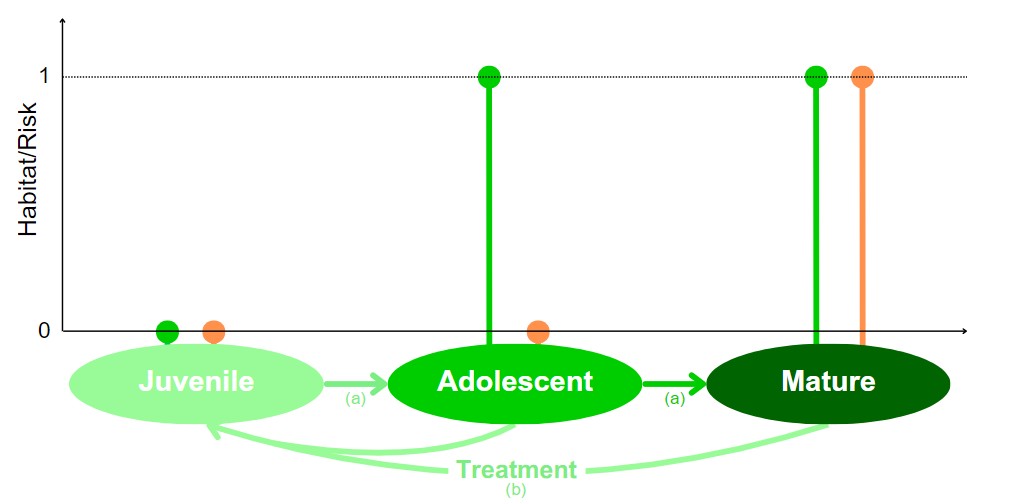
\includegraphics[width = .8\textwidth]{figures/wildland/Juvenile.png}
    \caption{Illustration of the successional stages and the link between successional stage, habitat and wildfire risk using a discretized Olson-type relationship}
    \subcaption*{At the bottom, the dynamics of the model are illustrated. First, successional stages transition (step (a)), then treatment is applied (step (b)). At the top, the link between successional stage, habitat and high risk. In green, a \textit{habitat} variables turns to $1$ when a cell is \textit{adolescent}, and in orange, a \textit{high risk} dummy turns to $1$ when a cell turns \textit{mature}} 
    \label{fig:illustration}
\end{figure}
%\end{minipage}%


%\subsection{Theoretical model}

We use a network structure to apprehend the landscapes. From the matrix $\mathbf{A}_t$, we form two graphs:  $\mathcal{B}_t = (V_{\mathcal{B}_t}, E_{\mathcal{B}_t})$, the graph of suitable habitat cells and $\mathcal{F}_t = (V_{\mathcal{F}_t}, E_{\mathcal{F}_t})$, the graph of high risk cells. First, the vertices of each graphs are the suitable habitat cells e.g $
V_{\mathcal{B}_t} = \{(i,j)$ such that $Habitat(a_{ijt})=1\}$ and the high risk cells, respectively e.g. $V_{\mathcal{F}_t} = \{(i,j)$ such that $Risk(a_{ijt})=1\}$.\\
Second, vertices are connected if they are within a Moore (or 8-cell) neighborhood of each other and share the same status. Therefore, notice that $\mathcal{F}_t\subset \mathcal{B}_t$. Figure \ref{fig:graph_overlap} illustrate the mechanism from the landscape in matrix form $\mathbf{A}_t$ with age classes ranging from 0 to 2, to graphs $\mathcal{B}_t$ and $\mathcal{F}_t$.

We use this 8-cell neighborhood for evaluating biodiversity habitat and wildfire risk within a common a spatial framework, using the same adjacency properties. 
Regarding biodiversity, we focus on general characteristics related to landscape structural connectivity rather than functional connectivity, as we are agnostic about effective species \citep{Fahrig2011}. We assume that species are able to disperse from one patch to another, and that habitat quality is uniformly distributed conditional on habitat being available.\\
We consider the wildfire risk through the lens of potential spread, influenced by fuel, wind direction and terrain. We abstract from wind patterns and terrain, to focus on fuel connectivity\footnote{Note that our framwork is amenable to prevailing wind patterns and terrain ruggedness, as the graph adjacency matrix can change from a Moore adjacency to any pattern influenced by environmental features}. Consistent with the literature (see \cite{Peterson_2009}, \cite{pais_cell2fire_2021, gonzalez-olabarria_fire_2023}), a wildfire can spread in any direction, conditional on neighbor cells with high risk. 

\begin{figure}
    \centering
    %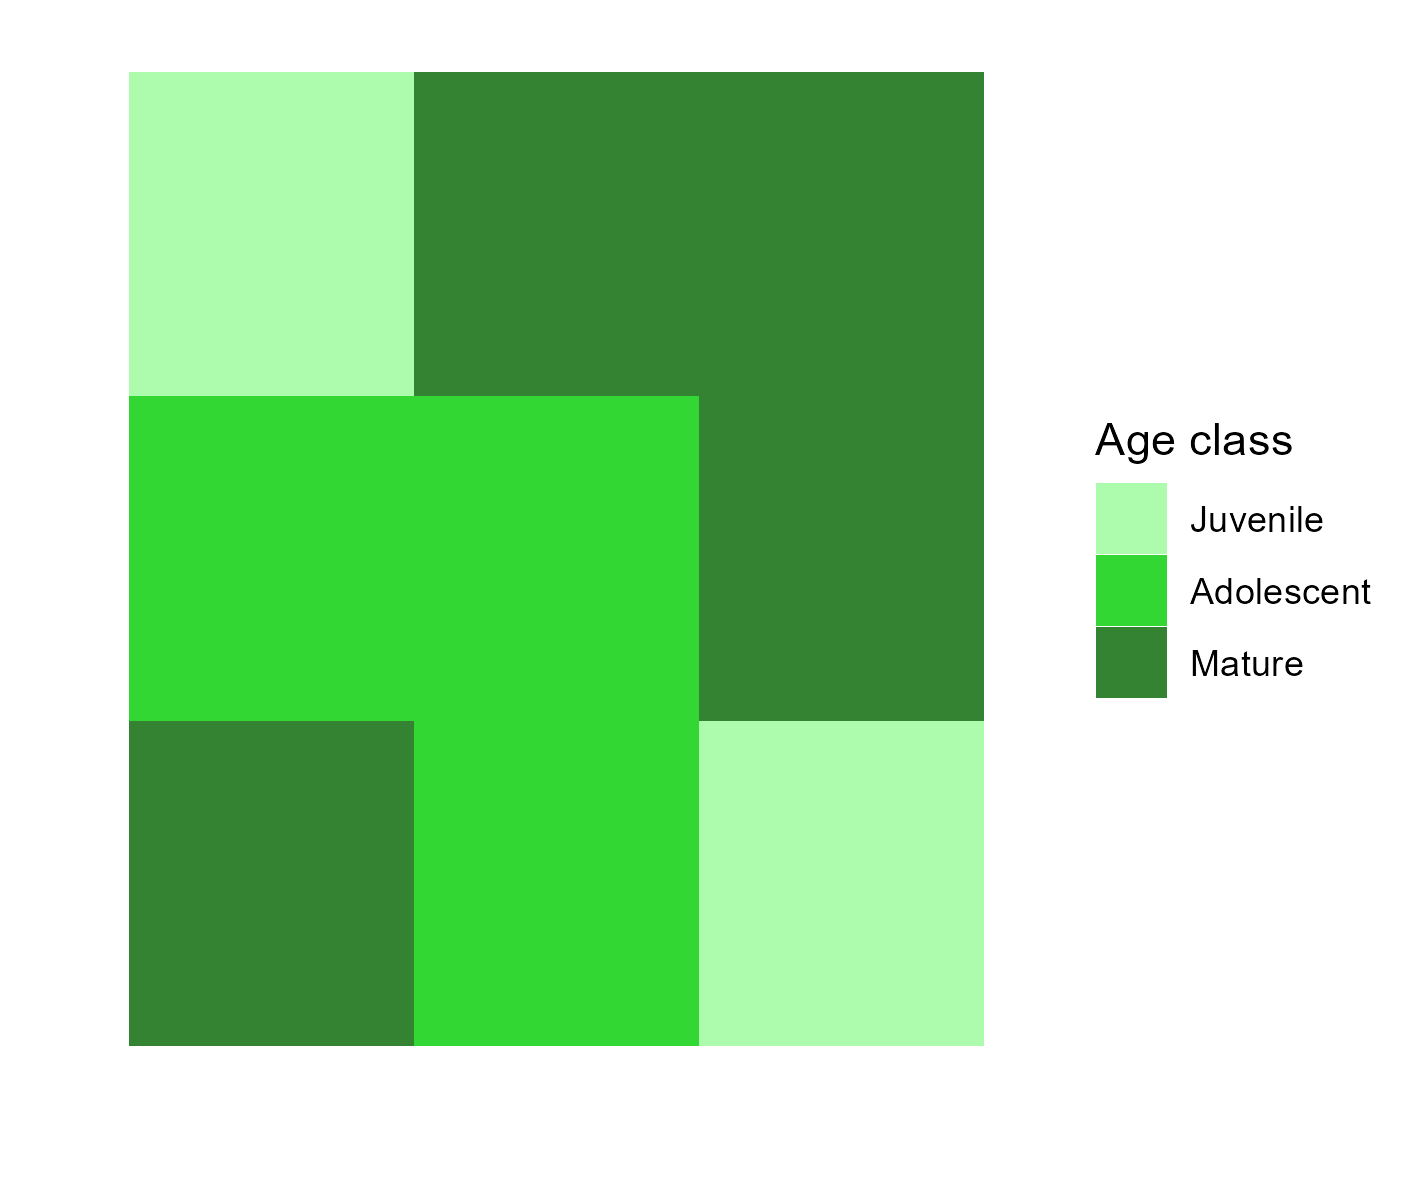
\includegraphics[width = .28\textwidth]{figures/wildland/illustration_from_raster.png}\\
    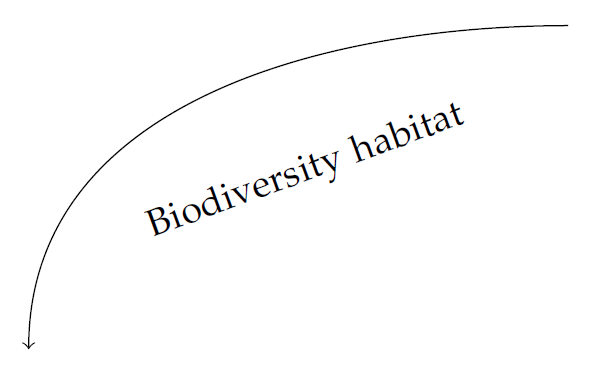
\includegraphics[width = 0.2\textwidth]{figures/wildland/arrow_biod2.PNG}
    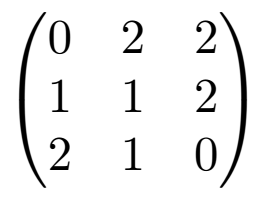
\includegraphics[width = 0.18\textwidth]{figures/wildland/land3.PNG}
    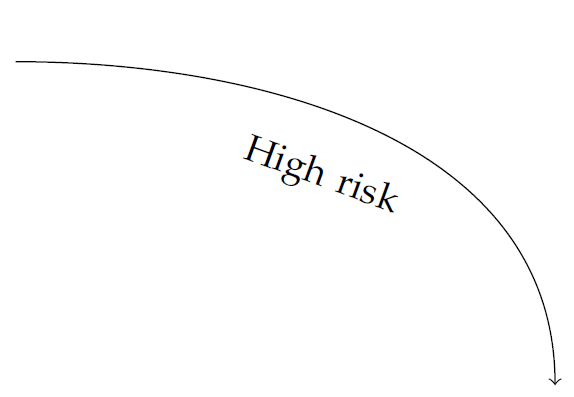
\includegraphics[width = 0.2\textwidth]{figures/wildland/arrow_fuel2.PNG}
    \\
    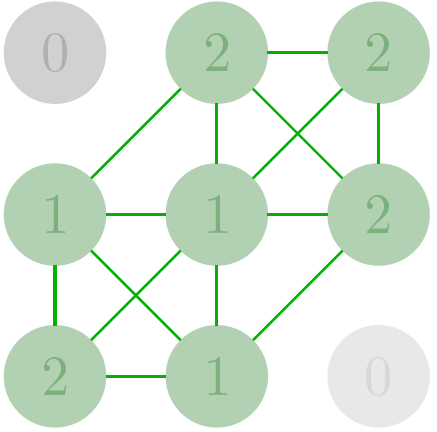
\includegraphics[width=0.2\textwidth]{figures/wildland/biodiv_3.PNG} \hspace*{4cm}
    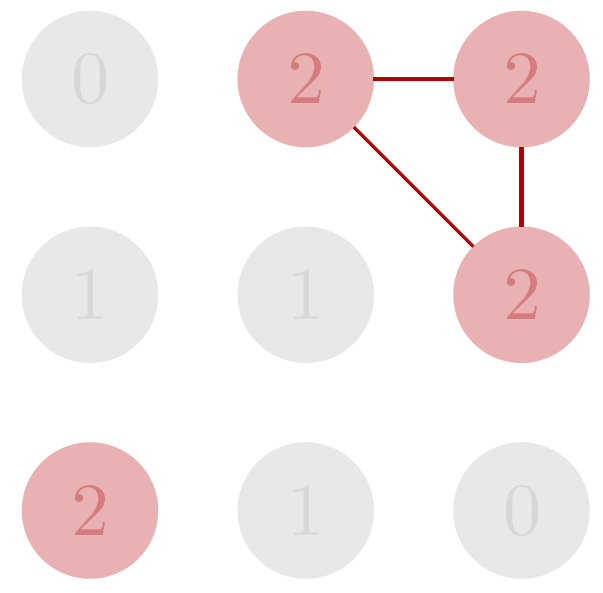
\includegraphics[width=0.2\textwidth]{figures/wildland/fire_3.PNG}\\
    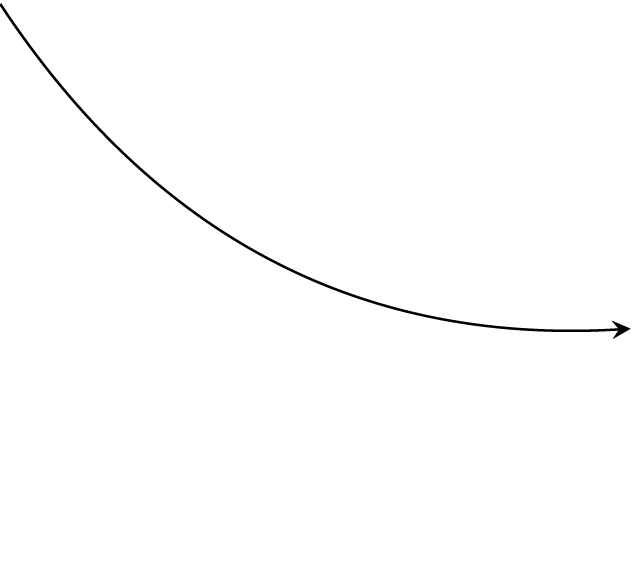
\includegraphics[width=0.18\textwidth]{figures/wildland/arrow_right.PNG}
    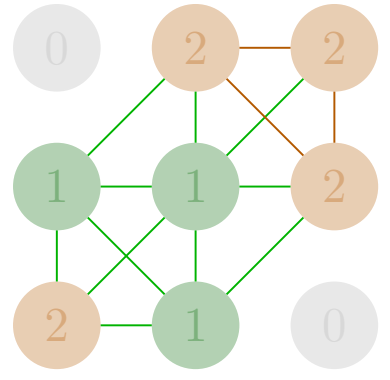
\includegraphics[width = 0.2\textwidth]{figures/wildland/graphe_feu_biod_33.PNG}
 	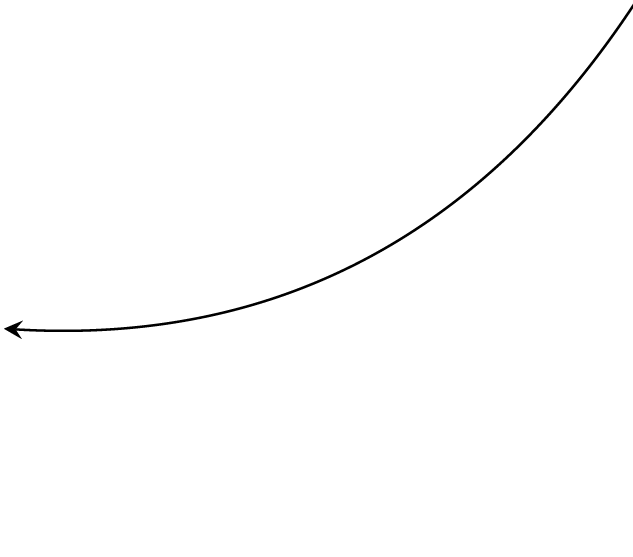
\includegraphics[width=0.18\textwidth]{figures/wildland/back_left.PNG}
    \caption{Illustration of the suitable habitat and high risk graphs for $n=3$}
    \subcaption*{The first layer is the values from a raster $\mathbf{A}_t$ of age classes in a forest landscape. It is turned into two different graphs. \\
In the left graph, the green vertices are $V_{\mathcal{B}_t}$ and support biodiversity habitat, while on the right graph, red vertices are $V_{\mathcal{F}_t}$ display high risk. Green and red links are respectively $E_{\mathcal{B}_t}$ and $E_{\mathcal{F}_t}$ \\
The high risk graph has two components (top right corner with 3 nodes, and bottom left corner with 1 node), while the biodiversity habitat graph only has one. \\
Cells for which the value is 0 are not considered as nodes for both graphs, and are thus not connected to the rest of the graphs. 
\\
In the final lansdcape, because $\mathcal{F}_t\subset \mathcal{B}_t$, the landscape  where orange cells are high fuel load and also support biodiversity habitat (e.g. $a_{ijt} \in V_{\mathcal{B}_t} \cap V_{\mathcal{F}_t}$)}
    \label{fig:graph_overlap}
\end{figure}

To assess the connectivity of $\mathcal{F}_t$ and $\mathcal{B}_t$, we use a global connectivity indicator. As connectivity can be measured in numerous ways in graph theory, we use this metric as is satisfies criteria pertaining to its evolution when vertices and edges are removed \citep{pascual-hortal_comparison_2006} when using graph theory applied to landscape ecology. Additionally, it offers a reformulation of the metric used in previous work closedly related to ours \citep{minas_spatial_2014, rachmawati_optimisation_2016} (see appendix \ref{sec:connectivity} for a demonstration). We define the global connectivity index of a given graph $\mathcal{G} = (\mathcal{V}, \mathcal{E})$ as\footnote{With $\mathrm{card}$ being the cardinal operator in set theory and denotes the number of elements in a set}:
\begin{equation}
H(\mathcal{G}) = \mathrm{card}(V) + 2\mathrm{card}(E)
\label{eq:high_connectivity}
\end{equation} 
Let a \textit{patch} be a collection of connected cells of suitable wildlife habitat.
This indicator considers that a habitat cell is connected to itself (i.e, within a habitat patch, there is no barrier) and whether it is connected to other cells.  
It implies lower connectivity when the distance between habitat cells increases, attains its maximum value when a single habitat patch covers the whole landscape, indicates lower connectivity as the habitat is progressively more fragmented, considers negative the loss of a connected or isolated cell, and detects as more important the loss of bigger patch, and less important steppingstone cells or patches. 
\\
Our global connectivity indicator is similar to the notion of \textit{energy of a graph} \citep{gutman_energy_2001}, which can be understood as a measure of connectedness (highly connected graphs tend to have high energy) for graphs. However, we differ from \cite{gutman_energy_2001} by including self-loops as habitat cells and patches are connected to themselves. Our formulation of $H$ reframes a quadratic form from the adjacency matrix of a graph grid structure (appendix \ref{sec:connectivity}). The adjacency matrix displays interaction among nodes that are neither purely constructive or destructive, as some combinations of active neighboring nodes will add to global connectivity, while other combinations may substract global connectivity. In all the landscape sizes we used, eigenvalues of the adjacency matrix were both positive and negative, leading to indefiniteness (see figure \ref{fig:eigenvalues}). Therefore, $H$ is not globally convex nor concave. 
\\
%and The vertices of $\mathcal{B}_t$ are cells that are at suitable habitat status (e.g. $Habitat(a_{it})=1$ and high risk status (e.g. $Risk(a_{it})=1$) and suitable habitat status
%
%We transform $A_t$ the set of cells constituting the landscape into graphs $G_t$ whose vertices $V_t$ (or nodes) are the cells in the landscape, and edges $E_t$ represent the connections between cells. We partition the landscape in two graphs, $G_{B_t}$ and $G_{F_t}$, each describing the network of mature habitat and risky patches (see fig. 1 for a representation). Landscape ecology has long used numerous, theoretically grounded indicators to analyze landscapes 
%
%\citep{urban_landscape_2001,minor_graph-theory_2008}. We use a global connectivity indicator that satisfies \cite{pascual-hortal_comparison_2006} criteria, grounded in graph theory, that offer a reformulation of \cite{rachmawati_optimisation_2016} (see Appendix \ref{sec:connectivity}). 
%Figure reference : \ref{fig:graph_overlap}
%
%We define cells to be connected if (i) they are within an 8-cell neighborhood and (ii) share the same status e.g. for a cell $i$, if cell $j$ is an 8-cell neighborhood (should we define it?)
%
%We define the global connectivity index of habitat and risky patches in landscape $A(t)$ as:
%
%This indicator considers that a habitat patch is connected to itself (i.e, within a habitat patch, there is no barrier) and whether it is connected to other patches.  
%It implies lower connectivity when the distance between patches increases, attains its maximum value when a single habitat patch covers the whole landscape, indicates lower connectivity as the habitat is progressively more fragmented, considers negative the loss of a connected or isolated patch, and detects as more important the loss of bigger patches, of key and less important steppingstone patches.
%
%We use a connectivity matrix to evaluate the ladnscape such that ...
%\textit{note that the framework is robust to changing the dispersal abilities. For example, one could think of (i) changing the dispersal abilities and (2) increase the size of the landscape to run applied stuff and (3) finding metrics to prioritize over species with different dispersal abilities. \textbf{This is a good discussion point : next work should include a variety of dispersal abilities and contributions to functional diversity to really dig deeper in this issue. }}
%\\\\

\subsection{Social planner decision : the high-risk /connectivity dilemma}
\subsubsection{Dynamic decision problem}
A social planner tries to minimize the global connectivity index of the high risk graph, using fuel treatments (eq. \ref{eq:objective}). However, when implementing treatment, a cell's successional stage is reset to \textit{juvenile}, thus destroying biodiversity habitat. In coherence with real world applications, the social planner is faced with a temporal budget constraint (e.g. the sum of treatments $\sum_{ij}x_{ijt}$ must be lower or equal to the $Budget$ - eq. \ref{const:budget}) as well as an ecological constraint, in terms of biodiversity habitat connectivity (e.g. the global connectivity of biodiversity habitat $H(\mathcal{B}_t)$ must be larger than constraint $Biod$ - eq. \ref{constr:biod}). Both the ecological and budget constraint need to be satisfied in each period.
\\
For the sake of the analysis, we focus on two layers of complexity : time and space. We do not include a stochastic component related to wildfire risk e.g. we adopt a deterministic framework where the value at risk (global connectivity of risky cells) is weighed against the loss in biodiversity habitat connectivity. Additionally, we consider a homogeneous distribution of treatment costs across the landscape e.g. cost of treatment in each cell through time is $1$. We come back to this assumption in the discussion. Monetary benefits are also homogenously distributed across the landscape, and normalized to 1. Note that there is, however, heterogeneous returns to treating across the landscape : some cells will contribute more than other to global connectivity. Finally, given that the planning horizon is finite, we do not discount future high risk connectivity scores and assume each period is equally important in decision making.

\clearpage

The optimization problem is : 

\begin{align}
    \min_{ \{\{x_{ijt}\}_{(i,j)}\}_{t=1}^T} & \left[ \sum_{t=1}^T H(\mathcal{F}_t)\right] \label{eq:objective}\\
\text{Such that: } & \notag \\
\mathbf{A}_0 &\text{ given} \label{eq:init_cond}\\
\forall t \in \{1, ..., T\} : & \notag \\
H(\mathcal{B}_t)&\geq Biod,\text{  }\label{constr:biod}\\
\text{ and }\forall (i,j) \in \{1,...,n\}   :& \notag \\
a_{ijt+1}& = \min((a_{ijt+1}(1-x_{ijt});2), \label{const:dyn}\\
 \sum_{i,j} x_{ijt} & \leq Budget,\text{  } \label{const:budget}\\
x_{ijt}&\in \{0,1\}\label{const:control}
\end{align}

\begin{table}[h]
\centering
\onehalfspacing
\resizebox{\textwidth}{!}{%
\begin{tabular}{|c|c|}
\hline
Notation & Concept \\
\hline \hline
$\mathbf{A}_t$ & Landscape matrix representing successional stage at time $t$ \\
$a_{ijt}$ & Cell $(i,j)$ of landscape with value $\in \{0,1,2\}$\\ 
$x_{ijt}$ & Treatment status $\in\{0,1\}$ of cell $(i,j)$ at time $t$ \\
$H$ & Global connectivity measure\\
$\mathcal{F}_t = (V_{\mathcal{F}_t}, E_{\mathcal{F}_t})$ & Graph of high risk cells\\
$\mathcal{B}_t = (V_{\mathcal{B}_t}, E_{\mathcal{B}_t})$ & Graph of suitable habit cells\\
\hline \hline
$Biod \in \{0,...,\max H(\mathcal{B})\}$ & Level of habitat global connectivity constraint\\
$Budget \in \{1,2,3,4\}$ & Level of the budget constraint\\
$n \in \{4,100\}$ & Size of the lansdcape\\
$c = 3$ & Number of age classes \\
$T \in \{5,10\} $ & Planning horizon\\
\hline 
\end{tabular}
}
\caption{Summary of model variables and functions}
\end{table}
%There are several reasons for this choice. First, the complexity of our problem is increasing in space and time, and in the number of initial conditions, as interpolation in a spatial setting is difficult given the behavior of our objective function. 
As common in the literature, we can express the budget as a share of land being treated ranging from %10\% to 33\% of the surface area (when $n=3$) and
5 to 25\% of the surface area (when $n=4$). These values encompass historical and projected policies in Australia \citep{burrows2013}, the United States \citep{GAO2019} and Southern Europe \citep{Fernandes2013}.
\\
Additionally, we solve the problem for a range of possible habitat connectivity values, ranging from $0$ to the maximum possible habitat connectivity for each landscape size $n$.

\clearpage
\subsubsection{Non-convexity and dimensionality curse}
Our problem can be classified as a \textit{critical node detection problem}, i.e, a problem of locating the vertices that best degrade connectivity, such that the number of components increase, and within remaining components, nodes with the largest \textit{centrality} are targeted \citep{ARULSELVAN20092193}. As definitions of \textit{graph centrality} matter, we refine our approach in section \ref{sec:treatment_centrality}.
Problems of the critical node class are computationally difficult (e.g. NP - Hard) in a single graph \citep{ARULSELVAN20092193, matsypura_wildfire_2018}. Efficient heuristics to find near-optimal solutions exist and leverage perturbations around local solutions \citep{ARULSELVAN20092193, Zhou2017}. Compared to the canonical \textit{critical node detection} problem, our problem features a non-convex objective function, a budget constraint, and a constraint on habitat connectivity, which imposes a constraint on the supergraph of high risk cells. Given our constraints, the behavior of the global connectivity measure $H$, standard optimization techniques cannot be applied, and heuristics are required. \\
%We solve the dynamic, integer program of the landscape manager
In dynamic problems, a standard technique is dynamic programming \citep{Bellman}. Dynamic programming provides a temporal decomposition of the initial problem defined over $T$ periods, into $T$ recursive problems, as it relies on the 'optimality principle'\footnote{"An optimal policy has the property that whatever the initial state and initial decision are, the remaining decisions must constitute an optimal policy with regard to the state resulting from the first decision". (See \cite{Bellman}, Chap. III.3., p.83)"}. A value function $V$, mapping each possible state of the world e.g. $\mathbf{A}_t$ to the optimal value of the objective function along the planning horizon, is iterated upon to find the optimal policies $x_{ijt}^*(\mathbf{A}_t)$, i.e, the sequence of optimal treatments, and the optimal states $\mathbf{A}_t^*(\mathbf{A}_0)$ resulting from the optimal policies and the initial conditions.
However, it is impractical in our case. Our problem suffers a \textit{dimensionality curse} \citep{Bellman}. There are $3^{n^2}$ values for the state variables \footnote{Given that the landscape $\mathbf{A}$ is of size $n\times n$, and that each element of $a_{ij}$ can take $c=3$ values, there are $3^{n^2}$ landcape configurations possible} in each period and the specific nature of our objective function $H$ (e.g. no global convexity) and the discrete nature of the state space make interpolation of a value function impossible \footnote{As a matter of fact, with a large number of state variables e.g. a high-dimensional state space, methods such as adaptive sparse grids can be used towith smooth, continuous objective functions \citep{brumm_adaptive_2017} to circumvent the dimensionality curse. The fact that the input space is an $n^2$-dimensional binary Cartesian product and that $H$ is not globally convex hinder the use of such tools.}.
%To manage the expected damages resulting from wildfires, the land planner can decide to undertake specific treatments, in the form of a combination of controlled burns and/or mechanical thinnings. Upon treatment, we assume that vegetation age in the cell is reset to 'absent': the wildfire risk vanishes, but so does the habitat and its connection to surrounding cells. Given the tension between maintaining habitat and reducing wildfire risk, the land planner aims to minimize a deterministic measure of connectivity of the high fuel loads in the landscape while maintaining a given level of biodiversity habitat connectivity under a budget constraint, over a planning horizon of length $T$. 
%For the sake of the analysis, we focus on two layers of complexity over time and space: global connectivity of high risk and biodiversity habitat. We do not consider stochastic wildfire behavior\textbf{point on risk and expected utility? } , heterogeneity in the economic costs or benefits (i.e, homogeneous treatment costs and no patch-specific asset to protect). The framework is however amenable to such a prioritization. We also assume that the budget cannot be banked, and has to be utilized in each period, consistent with operational rules. Moreover, as the budget is constrained in each period, the measure of risk is bounded and the planning horizon is finite, we rule out discounting and assume each generation matters as much to the social planner. 
%We abstract from decision-making in a risky environment, as it has been extensively described in economics and decision theory \citep{Mouysset2013}. Moreover, we mimic the role of risk aversion by varying the level of habitat connectivity constraint the decision maker chooses. 
%If ignition is a binary process in each period, the probability of which is independent of the high-risk graph properties, our model can be viewed as minimizing an upper bound of the expected losses from wildfires (see appendix).

\clearpage
\subsection{Solution method and computational experiments}

Three key features of our problem hint that a dynamic (e.g. that optimizes the objective function over the whole planning horizon) and a repeated myopic solution (e.g. which optimizes the objective function in each period)  should be similar. The dynamics occur before the decision is made, therefore the decision maker has full knowledge about the state of the system. The dynamics are simplified and have relatively little depth, as we limit ourselves to 3 age classes. Finally, our intertemporal objective function is additively separable.

Our solution methods resort to two key ingredients : optimization heuristics, and comparison between the dynamic and repeated myopic problem. \\
First, we circumvent the non-convexity of the global connectivity metric and the high dimension of the state space by using a genetic algorithm \citep{holland_adaptation_1975} (implemented in \textsf{R} with package \texttt{GA} \citep{GA_2017}) with population size of $200$ and $250$ iterations. Genetic algorithms are especially suited for high dimensional, combinatorial search spaces\footnote{Here, the control variable is a $Tn^2 = 5n^2$ binary variable} and fare better than a brute force approach, or other heuristics (Particle Swarm Optimization or Simulated Annealing). 
\\
Then, we compare the performance of a 5-period objective function to a 5 period repetition of a static objective function. We trade the completeness of dynamic programming for a more manageable approach, where we compare these approaches for %$696$ and 
$884$ randomly drawn landscapes of size $n=4$.
% $n \in \{3,4\}$. 
We sample the landscapes according to the 
distribution of possible landscapes (see figure \ref{fig:appendix_distribution}). As landscapes with large numbers of \textit{juvenile} and \textit{adolescent} cells are overrepresented, we impose that underrepresented possible landscapes are included at least 2 times in our sample, to disentangle composition (e.g. number of cells of each successional stage) from configuration (location of cells) effects.

 We focus $T=5$ planning horizon for several reasons. First, as the dynamic of our ecological processes comprises 3 stages, using a 5-period horizon allows for each cell to grow from its original stage to \textit{mature}, be treated, and revert to its original stage, e.g. allows for a full successional cycle to be performed. Second, a 5-period horizon corresponds to a long policy horizon, ranging from 25 years to 200 years \citep{mccoll_gausden_pathways_2019, thomas_wildlife_1979}.
Third, for our approach to be useful for policy making given that we abstract from stochastic modifications to the environment (e.g. occurence of wildfire, spread of invasive species increasing flamability at a given age etc), policies need to be forward looking with enough temporal depth to be relevant and be reevaluated with potentially new initial conditions resulting from environmental perturbations.\\
%
Next, with repeated static optimization we increase the size of our sample and temporal depth, to encompass all the possible landscape configurations for landscape size $n=4$,
%$n \in \{3, 4\}$, 
over the whole range of possible values for the biodiversity habitat constraint, over $T=10$ years. 
Of all the $3^{n^2}$ initial landscapes combinations possible, we only keep landscapes that are unique up to a permutation\footnote{That is to say, landscape $\mathbf{A}_0$ is included in the set of initial conditions $\mathcal{I}$ if and only if for any element $\mathbf{A'}_0$ in $\mathcal{I}$, $\mathbf{A}_0$ is not a permutation (eg can be obtained through rotations or symmetries) of $\mathbf{A'}_0$}. This results in a sharp reduction of landscapes to consider
%from $19,683$ initial conditions to $2861$ unique initial landscapes for $n=3$, and 
from $43,046,721$ initial to $5,398,082$ unique initial landscapes for $n=4$. We focus on exact optimal solutions for all the initial conditions of these small-scale landscapes and implement our own solution algorithm in Python 3.9.13 and R 4.3.3\footnote{Data and code are \href{https://github.com/sim-jean/Landscape_connectivity_dilemma}{publicly available}}. We find generally applicable principles for treatment allocation.
\\
Third, we increase the landscape size to $n=100$, for a sample of 20 large scale (10,000 cells) landscapes with varying compositions and autocorrelation using two-dimensional fractional Brownian motions  (table \ref{tab:composition_nlm} summarizes their characteristics and figure \ref{fig:ex_nlm} illustrates 6 of them). We use neutral landscape models \citep{caswell_community_1976, gardner_neutral_2007} and implement them in \textsf{R} \citep{sciaini_nlmr_2018}. Neutral landscape models were designed in theoretical landscape ecology to develop spatial ecology indicators and ``evaluate the effects of landscape structure on ecological processes'' \citep{with_neutral_1997}. Even though they are designed as null models to compare with real landscapes, after ecological processes have shaped them, they provide a useful basis for scaling our analysis. We solve the repeated myopic optimization problem on these 20 landscapes over $T=10$ periods based on our generally applicable principles, and compare them with other policy scenarios.
We compare our principles with (i) a repeated random policy, targeting cells that are either \textit{adolescent} or \textit{mature}, (ii) a gridded treatment policy (as depicted in figure \ref{fig:grid}) with evenly spaced segments of treatment, (iii) a policy that always targets the most central nodes in terms of betweenness centrality, and (iv) a policy which targets the largest degree\footnote{In a graph $\mathcal{G}=(V,E)$, the degree of a node $v$ is the number of edges connected to the node} nodes, in terms of global risk and habitat connectivity measures.
%
%
%\subsubsection{Non-convexity and dimensionality curse}
%Our problem can be classified as a \textit{critical node detection problem}, i.e, a problem of locating the vertices that best degrade our global connectivity metric $H(\mathcal{F}_t)$ \citep{ARULSELVAN20092193}. Problems of the critical node class are computationally difficult (e.g. NP - Hard) in a single graph \citep{ARULSELVAN20092193, matsypura_wildfire_2018}. Efficient heuristics to find near-optimal solutions exist and leverage perturbations around local solutions \citep{ARULSELVAN20092193, Zhou2017}. Compared to the canonical \textit{critical node detection} problem, our problem features non-convex objective function, a budget constraint, and a constraint on habitat connectivity, which imposes a constraint on the supergraph of high risk cells. Given our constraints, the behavior of the global connectivity measure $H$, standard optimization techniques cannot be applied. \\
%We solve the dynamic, integer program of the landscape manager
%In dynamic problems, a standard technique is dynamic programming. Dynamic programming provides a temporal decomposition of the initial problem defined over $T$ periods, into $T$ recursive problems, as it relies on the 'optimality principle'\footnote{"An optimal policy has the property that whatever the initial state and initial decision are, the remaining decisions must constitute an optimal policy with regard to the state resulting from the first decision". (See \cite{Bellman}, Chap. III.3., p.83)"}. A value function $V$, mapping each possible state of the world e.g. $\mathbf{A}_t$ to its objective function value, is iterated upon to find the optimal policies $x_{ijt}^*(\mathbf{A}_t)$, i.e, the sequence of optimal controlled burns, and the optimal states $\mathbf{A}_t^*(\mathbf{A}_0)$ resulting from the optimal policies and the initial conditions.
%However, it is impractical in our case. As a matter of fact, our problem suffers a \textit{dimensionality curse} \citep{Bellman}. There are $3^{n^2}$ possible combinations\footnote{Given that the landscape $\mathbf{A}$ is of size $n\times n$, and that each element of $a_{ij}$ can take $c=3$ values, there are $3^{n^2}$ landcape configurations possible} in each period and the specific nature of our objective function $H$, the habitat connectivity and budget constraints make interpolation of a value function impossible \footnote{As a matter of fact, even with a large number of state variables e.g. a high-dimensional state space, adaptive sparse grids can be used with smooth, continuous objective functions \citep{brumm_adaptive_2017}. The fact that the input space is an $n^2$-dimensional binary Cartesian product and that $H$ is not globally convex hinder the use of such tools.}. 
%
%Nonetheless, three key features of our problem hint that dynamic and repeated myopic solutions should be similar. The dynamics occur before the decision is made, therefore the decision maker has full knowledge about the state of the system. The dynamics are simplified and have relatively little depth, as we limit ourselves to 3 age classes. Finally, our intertemporal objective function is additively separable.
%
%
%
%\subsubsection{Dynamic v. repeated myopic solutions}
% 
%To circumvent this issue, we adopt a three-fold approach. \\
%First, we trade the completeness of dynamic programming (e.g. solution of the problem for the entire domain of the state variable $\mathbf{A}$) for a manageable piecemeal approach, where we solve the complex 5-period combinatorial problem with a genetic algorithm \citep{holland_adaptation_1975} (implemented in \textsf{R} with package \textit{GA} \citep{GA_2017}) for 300 randomly generated landscapes, with population size of $200$ and $250$ iterations. Genetic algorithms are especially suited for high dimensional, combinatorial search spaces\footnote{Here, the control variable is a $Tn^2 = 5n^2$ binary variable} and fare better than a brute force approach, or other heuristics (Particle Swarm Optimization or Simulated Annealing). 
%
%Three key features of our problem hint that dynamic and repeated myopic solutions should be similar. The dynamics occur before the decision is made, therefore the decision maker has full knowledge about the state of the system. The dynamics are simplified and have relatively little depth, as we limit ourselves to 3 age classes. Finally, our intertemporal objective function is additively separable.
%Hence, we compare the performance of the 5 period, genetic algorithm approach to a repeated static optimization procedure, for landscapes of size $n\in\{3,4\}$. While this size appears simplifying, it encapsulates the main mechanisms displayed in similar models \citep{rachmawati_optimisation_2016, rachmawati_fuel_2018}. Based on these results, we increase the planning horizon to
%\\
%\textbf{Comment est ce qu'on dit ici qu'on accroit peut être l'horizon?}
%Second, we perform a repeated static optimization on all the possible landscape configurations for landscape size $n \in \{3, 4\}$, over all the whole range of possible values for the biodiversity habitat constraint, over 5 years. This approach sacrifices the dynamics of our problem but allows us to scan the entire state space to gain insights.
%Of all the $3^{n^2}$ initial landscapes combinations possible, we only keep landscapes that are unique up to a permutation\footnote{That is to say, landscape $\mathbf{A}_0$ is included in the set of initial conditions $\mathcal{I}$ if and only if for any element $\mathbf{A'}_0$ in $\mathcal{I}$, $\mathbf{A}_0$ is not a permutation (eg can be obtained through rotations or symmetries) of $\mathbf{A'}_0$}. This results in a sharp reduction of landscapes to consider, from $19,683$ initial conditions to $2861$ unique initial landscapes for $n=3$, and from $43,046,721$ initial to $5,398,082$ unique initial landscapes for $n=4$. We focus on exact optimal solutions for all the initial conditions of these small-scale landscapes and implement our own solution algorithm in Python 3.9.13 and R 4.3.3\footnote{Data and code are \href{https://github.com/sim-jean/Landscape_connectivity_dilemma}{publicly available}}.
%\\
%Third, we simulate 20 large scale (10,000 cells) landscapes with varying compositions and autocorrelation using two-dimensional fractional Brownian motions  (table \ref{tab:composition_nlm} summarizes their characteristics and figure \ref{fig:ex_nlm} illustrates 6 of them). We use neutral landscape models \citep{caswell_community_1976, gardner_neutral_2007} and implement them in \textsf{R} \citep{sciaini_nlmr_2018}. Neutral landscape models were designed in theoretical landscape ecology to develop spatial ecology indicators and ``evaluate the effects of landscape structure on ecological processes'' \citep{with_neutral_1997}. Even though they are designed as null models to compare with real landscapes, after ecological processes have shaped them, they provide a useful basis for scaling our analysis. We solve the repeated myopic optimization problem on these 20 landscapes.
%
%using dynamic programming. Dynamic programming provides a temporal decomposition of the initial problem defined over $T$ periods, into $T$ recursive problems, as it relies on the 'optimality principle'\footnote{"An optimal policy has the property that whatever the initial state and initial decision are, the remaining decisions must constitute an optimal policy with regard to the state resulting from the first decision". (See \cite{Bellman}, Chap. III.3., p.83)"}.  The outputs of the method are both the optimal policies $x_j^*(t,A)$, i.e, the sequence of optimal controlled burns, and the optimal states $A_j^*(t,A_0)$ resulting from the optimal policies and the initial conditions. Moreover, we solve a repeated myopic optimization procedure, where in each time step, the decision maker minimizes the current global connectivity measure of high risk cells, under constraints \ref{eq:init_cond}-\ref{const:control}. In the dynamic problem, the biodiversity habitat and budget constraints gradually restrict the solution space, and limit the extent to which system dynamics (e.g the appraisal of long terms successional stages across the landscape) may impact optimal solutions. We compare the repeated myopic solution to the dynamic solution.
%
%\subsubsection{Circumventing non-convexity and dimensionality curse}
%
%Our problem can be classified as a \textit{critical node detection problem}, i.e, a problem of locating the vertices that best degrade our global connectivity metric $H(\mathcal{F}_t)$ \citep{ARULSELVAN20092193}. Problems of the critical node class are computationally difficult (e.g. NP - Hard) in a single graph \citep{ARULSELVAN20092193, matsypura_wildfire_2018}. Efficient heuristics to find near-optimal solutions exist and leverage perturbations around local solutions \citep{ARULSELVAN20092193, Zhou2017}. Our problem is a constrained, integer optimization problem with a non-convex objective function,
%that constrains not only the set of nodes to be removed but also metrics relative to a larger graph structure e.g. the supergraph of high risk cells, biodiversity habitat. Given the behavior of the global connectivity measure $H$, standard optimization techniques cannot be applied. \\
%Additionally, the complexity of our combinatorial problem increases with landscape size $n$, the number of vegetation age classes $c$, and time $T$ i.e. features a \textit{dimensionality curse} \citep{Bellman}: there are $c^{n^2}$ eg. $3^{n^2}$ initial landscape configurations possible, and given an initial landscape, there are $n^2 \times T$ possible treatment allocations to be considered. 
%To circumvent these issues, we use a genetic algorithm \citep{holland_adaptation_1975} (implemented in \textsf{R} with package \textit{GA} \citep{GA_2017}). Compared to other heuristics, such as Particle Swarm Optimization or Simulated Annealing, genetic algorithms fare better on high dimension, combinatorial search spaces. With small scale landscapes (e.g. $n\in \{3,4\}$), we use a population size of $100$ individuals with $250$ iterations which guarantees that the heuristic converges to a near optimal solution.
%
%Moreover, as the objective function is neither globally convex nor concave, and the structure of the optimization problem is constrained, we required large test populations for our genetic algorithm to avoid getting stuck in local minima.  es.
%
%\subsubsection{Small and large scale repeated myopic optimization}
%
%We limit ourselves to studying the initial conditions in landscapes of size $n=3$ and $4$. While this formulation appears simplifying, it encapsulates the main mechanisms displayed in similar models \citep{rachmawati_optimisation_2016, rachmawati_fuel_2018}.\\
%First, we solve the dynamic problem and repeated static problem for 300 randomly selected initial landscapes.
%Then, we focus on all the possible landscape combinations of size $n \in \{3,4\}$ using repeated myopic optimization, over all the whole range of possible values for the biodiversity habitat constraint, over 5 years. \\
%Of all the $3^{n^2}$ initial landscapes combinations possible, we only keep landscapes that are unique up to a permutation\footnote{That is to say, landscape $\mathbf{A}_0$ is included in the set of initial conditions $\mathcal{I}$ if and only if for any element $\mathbf{A'}_0$ in $\mathcal{I}$, $\mathbf{A}_0$ is not a permutation (eg can be obtained through rotations or symmetries) of $\mathbf{A'}_0$}. This results in a sharp reduction of landscapes to consider, from $19,683$ initial conditions to $2861$ unique initial landscapes for $n=3$, and from $43,046,721$ initial to $5,398,082$ unique initial landscapes for $n=4$. We focus on exact optimal solutions for all the initial conditions of these small-scale landscapes and implement our own solution algorithm in Python 3.9.13 and R 4.3.3\footnote{Data and code are \href{https://github.com/sim-jean/Landscape_connectivity_dilemma}{publicly available}}.
%
%
%
%Finally, we simulate 20 large scale (10,000 cells) landscapes with varying compositions and autocorrelation using two-dimensional fractional Brownian motions  (table \ref{tab:composition_nlm} summarizes their characteristics and figure \ref{fig:ex_nlm} illustrates 6 of them). We use neutral landscape models \citep{caswell_community_1976, gardner_neutral_2007} and implement them in \textsf{R} \citep{sciaini_nlmr_2018}. Neutral landscape models were designed in theoretical landscape ecology to develop spatial ecology indicators and ``evaluate the effects of landscape structure on ecological processes'' \citep{with_neutral_1997}. Even though they are designed as null models to compare with real landscapes, after ecological processes have shaped them, they provide a useful basis for scaling our analysis. We solve the repeated myopic optimization problem on these 20 landscapes.
%
%
\subsection{Lanscape and treatment indicators}
\label{section:indicators}
\subsubsection{Landscape level indicators}
To characterize the managed landscapes, we mobilize several indicators from landscape ecology and graph theory (see appendix \ref{sec:appendix_wildland__indicators}).

First, we account for the high risk and habitat surfaces in the landscape by measuring the number of vertices in each graph.
Second, to assess landscape connectivity and fragmentation as well as landscape diversity\footnote{In the context of fire prone ecosystems, the notion of ``fire mosaics'' \citep{bradstock_which_2005} conveys the idea that fire causes variations in successional stages through space thus providing different types of habitat for biodiversity and improving biodiversity}, we use our global connectivity metric $H$ (eq. \ref{eq:high_connectivity}), as well as the \textit{number of components}\footnote{A \textit{component $\mathcal{C}_t$} of graph $\mathcal{G}_t$ is a maximally connected subgraph of $\mathcal{G}_t$ that is not part of any larger connected subgraph. A component is \textit{connected} (for all two vertices $(u,v) \in V_{\mathcal{C}}$, there exists a path in $\mathcal{C}_t$ that connects them) and $\mathcal{C}_t$ being a subgraph of $\mathcal{G}_t$, it is \textit{maximal} if there is no other connected subgraph $\mathcal{C'}$ of $\mathcal{G}_t$ such that $\mathcal{C}_t$ is a proper subgraph of $\mathcal{C'}_t$. Figure \ref{fig:graph_overlap} illustrates this concepts in both the habitat and high risk graphs resp. $\mathcal{B}_t$ and $\mathcal{F}_t$}.
To specifically assess landscape diversity, we use the Simpson index \citep{simpson_measurement_1949} on successional stages stages (eq. \ref{eq:simpson})\footnote{Similar results can be found with the Shannon index \citep{Shannon1949}. To avoid issues related to degenerate values and logarithms, we focus on the Simpson index.}. 
However, the Simpson index does not account for the diversity of spatial patterns: a checkered landscape with two seral stages would be as diverse as a landscape with two large patches for each seral stage, according to the Simpson index. Therefore, we use the landscape shape index (LSI - eq. \ref{eq:LSI}), a normalized ratio between the perimeter of biodiversity habitat and its area \citep{patton_diversity_1975, McGarigal_1995}.
%\begin{equation}
%LSI = \frac{perimeter(\mathcal{G}_t)}{4n} \text{ such that }\mathcal{G}_t \in \{\mathcal{B}_t,\mathcal{F}_t\}
%\end{equation}
To disentangle the correlated effects of perimeter and area that affect the landscape shape index, we use a successional stage heterogeneity index, that averages the probability that, for each cell, neighbors in the 4 cardinal directions share the same successional stage (eq. \ref{eq:lth_index}). The index ranges between 0, when the successional stage is the same across the whole landscape, to 1, in a checkered landscape. The index assesses whether the landscape is a mosaic \citep{bradstock_which_2005}, and if it displays structural diversity, conducive to diverse communities and functional diversity. 

\subsubsection{Treatment level indicators}
\label{sec:treatment_centrality}
To analyze the treatment allocation mechanism, we use the \textit{number of treatments} as well as their \textit{geographic location}. Additionally, we use graph theory measures to assess the location of treatments in relation with the graph structure. To do so, we use different measures of \textit{centrality}, e.g. measures that answer how important a vertex is for the graph structure, and overall, its connectivity. Measures of centrality produce a ranking of vertices, but are not necessarily comparable. Additionally, depending on the measure chosen, different vertices can be the most central. To overcome these limitations, we use 4 measures of vertex centrality. 

First, we use \textit{degree centrality}, which measures the degree of vertices. This measure is computationally simple and captures direct centrality effects e.g. how a single vertex interacts with its neighbors, without considering 2nd degree neighbors, or further relationships. Second, we use \textit{betweenness centrality} (see appendix \ref{sec:treatment_centrality_appendix} for a formal definition), measuring the extent to which a vertex in on the shortest path between other vertices. This measure is more computationally intensive and  useful to understand through which vertex flows may go through, e.g. wildlife dispersal or wildfire spread. Third, we use \textit{eigencentrality}, which measures the influence of nodes through their connections : a vertex is central if it is largely connected to nodes themselves well-connected. While computationally intensive, it furthers the results from degree centrality. Finally, we use \textit{subgraph centrality} \citep{estrada_subgraph_2005}, which measures the participation of vertices to subgraphs of the graph, and captures the role of a node in local structures, especially suited for networks with well identified, low connected subgraphs. We implement these measures in $\textsf{R}$ using the package \texttt{igraph} \citep{Csrdi2006TheIS}



\section{Results}

\subsection{Dynamic v. myopic repeated optimizations}

As expected, the results of the dynamic and static optimization procedures over 5 periods yield very similar aggregate results in terms of intertemporal global risk connectivity (hereafter \textit {risk}), for different budget (measured in treatment units) and global habitat connectivity constraints (hereafter \textit{habitat constraints}, measured as proportion of the maximal global habitat connectivity attainable), as shown by figure \ref{fig:risk_diff}.

\begin{figure}[h]
    \centering
    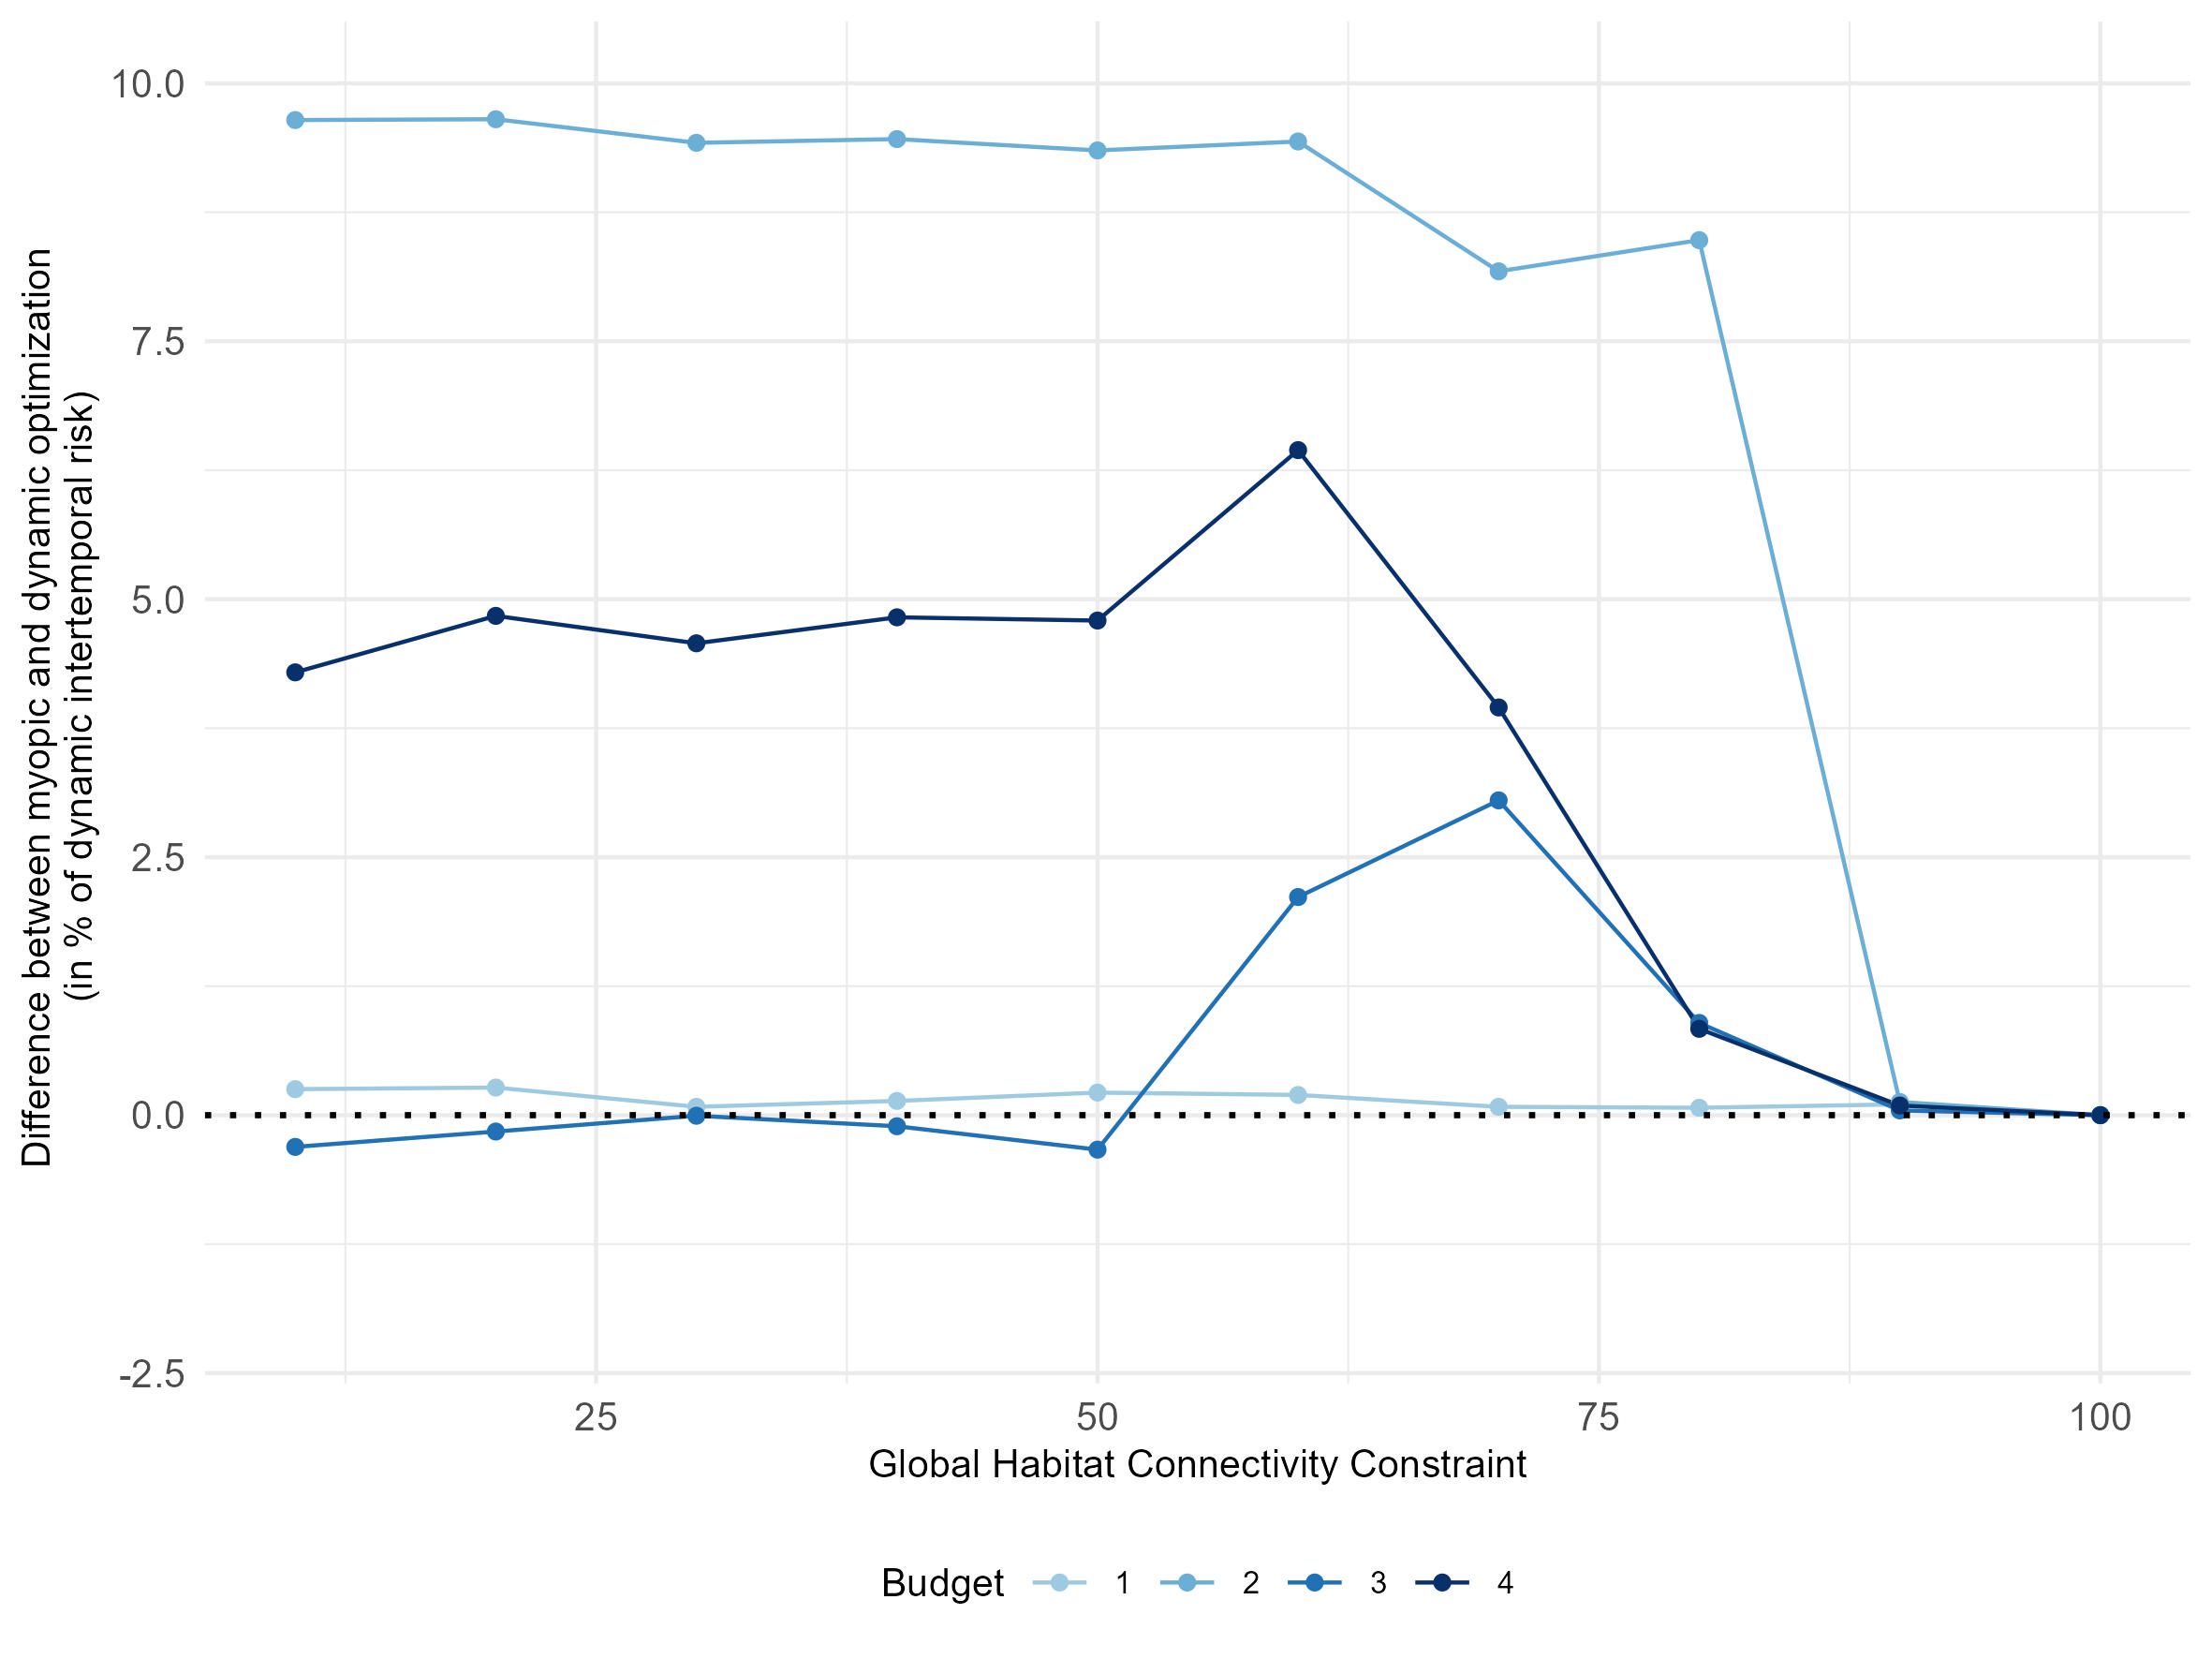
\includegraphics[width = .8\linewidth]{figures/wildland/aggregate_risk_diff.jpg}
    \caption{Comparison of aggregate intertemporal global risk connectivity for dynamic and repeated myopic procedures}
    \label{fig:risk_diff}
\end{figure}
 
Table \ref{tab:lm_risk} shows the result of a regression analysis of the difference in global risk connectivity between the dynamic optimization and the repeated myopic procedure (e.g. if the difference is positive, repeated optimization results in a lower intertemporal global risk connectivity), based on initial landscape characteristics, without interaction terms. First, the average risk difference is positive across all habitat constraint levels (given the magnitude of the intercept and constraint coefficients). With larger budgets, the relative performance of repeated myopic optimization increases, while it merely decreases with increases in the habitat connectivity constraint level: although statistically significant, the magnitude is negligble. Finally, the Successional Stage Heterogeneity Index is statistically significant but does not lead to significant effects due to its magnitude. Other models, including interaction terms are presented in appendix \ref{sec:appendix_reg}. They all point towards the absence of clear mechanism determining the performance differentials between myopic and dynamic optimization procedures.


\FloatBarrier

\subsection{Wildfire risk reduction and habitat connectivity : a production possibility frontier approach}

Figure \ref{fig:frontier} shows the global risk connectivity measure, with varying levels of global habitat connectivity and budget constraint, e.g. a production possibility frontier between risk and habitat connectivity, for the 10 years planning horizon\footnote{Figure \ref{fig:appendix_fpp_dyn_myopic} displays production possibility frontiers for repeated myopic and dynamci procedures and shows the same properties}

\begin{figure}[h]
    \centering
    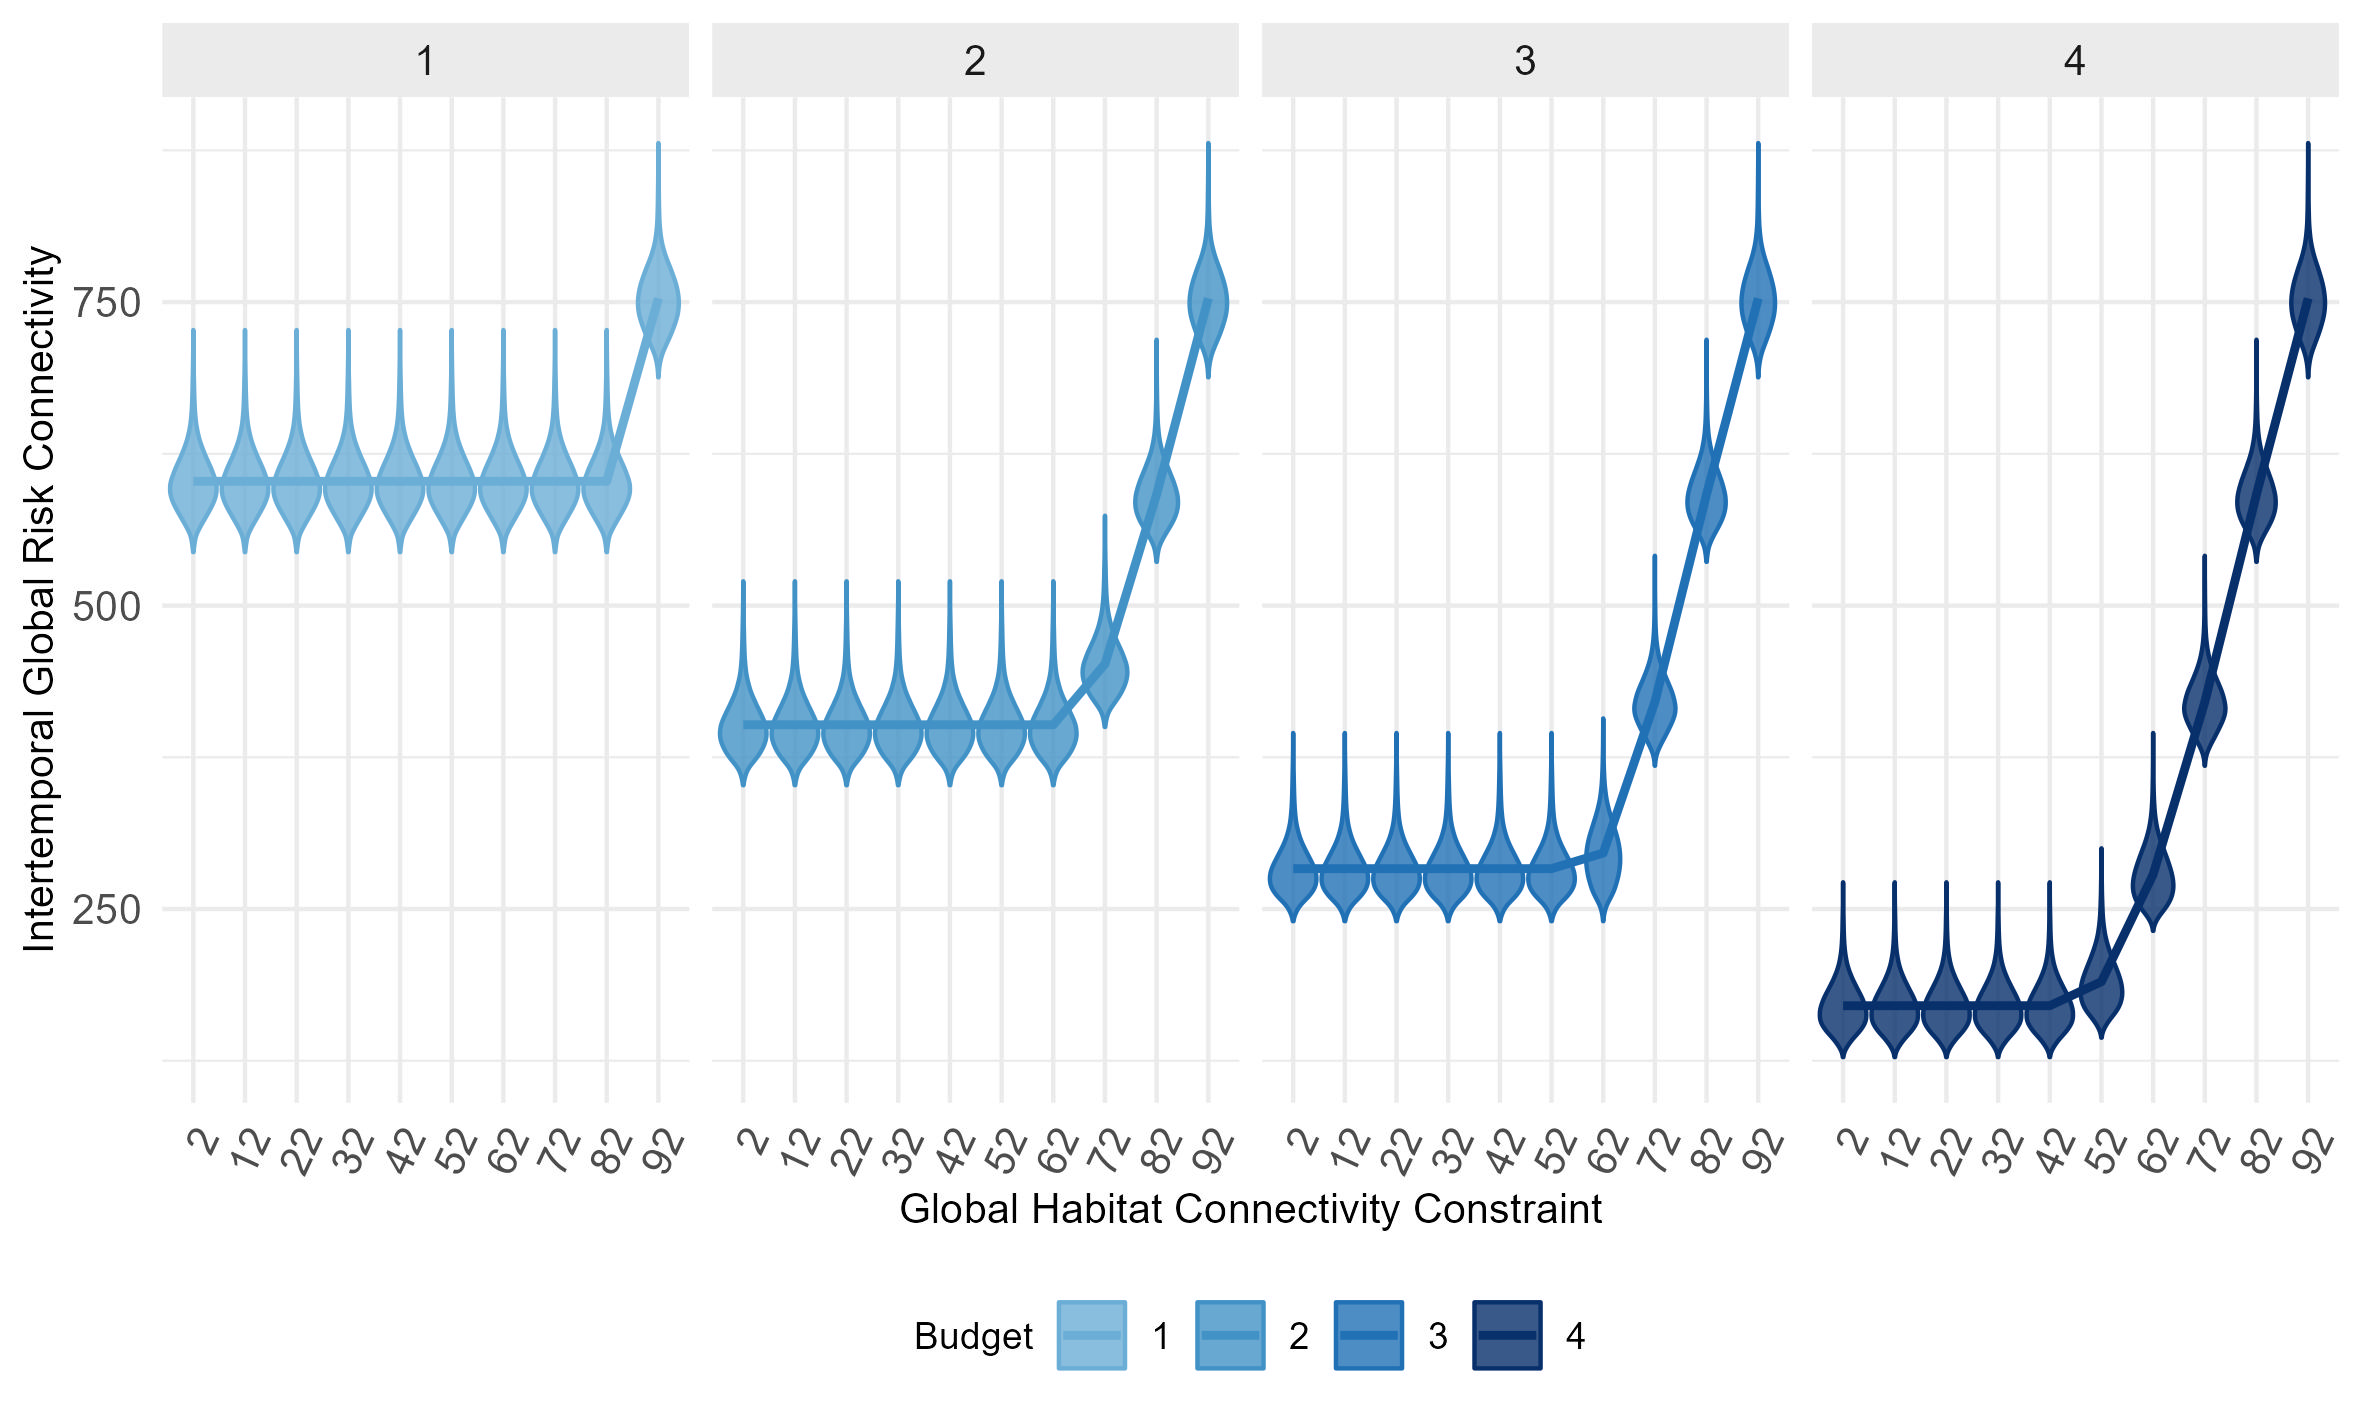
\includegraphics[width = .8\textwidth]{figures/wildland/fpp.jpg}
    \caption{Production possibility frontier across global habitat connectivity and budget constraints}
    \subcaption*{For each value of the global habitat connectivity constraint is plotted the distribution of the values in each violin plot. The line refers to the group specific average level of global risk connectivity}
    \label{fig:frontier}
\end{figure}

Using repeated myopic spatial optimization, reducing global risk connectivity while maintaining global habitat connectivity comes as a trade-off, albeit moderate: indeed, increasing habitat requirements increases the remaining risk, but there are combinations that can satisfy large habitat connectivity and risk reductions. 

Budget is a key factor in risk reduction, as it relaxes the trade-off between the two objectives: increasing the budget reduces the wildfire risk while maintaining a range of biodiversity constraints.  When habitat constraints are large, however, the marginal effect of budget is limited, production possibility frontiers tend to be identical and a larger remaining risk needs to be accepted.  Indeed, when the $Budget =2$, average risk is maintained at $401$ for habitat constraint levels ranging from 2 to 62, while when $Budget=4$, risk is down to $170 (-58\%)$ for habitat constraint levels ranging from 2 to 42.  
However, when the habitat constraint is at 72, average risk for $Budget=2$ is at $451$, while it is at $420$ for $Budget=4$ (7\% difference). Hence, similar risk profiles can be attained at a lower budget for high habitat constraints. 
Conversely, as the costs of treatment increase, for a stable budget, the remaining risk increases sharply, and factoring in habitat requirements in the decision-making is not necessary for targets below 82. For example, if costs were to double at $Budget=2$, the average risk between 2 and 62 would increase by 50\% (e.g. at $Budget=2$, average risk is $401$, while it is $602$ for $Budget=1$), and the habitat constraint only becomes stringent at $82$. 
%\textbf{Pas sur de ça, un peu gros peut être?} Our results suggest that in the face of climate change if treatment costs increase, focusing on reducing wildfire risk should be a priority and would accommodate wildlife habitat. 
%\textbf{Point sur l'importance de la spatialisation? i.e, meilleur score vs random? ou focus sur un seral stage?}

\FloatBarrier
\subsection{Convergence towards steady states}
Our simulations for $T=10$ and scanning all the possible configurations for landscapes of size $n=4$ show that 100\% of the initial landscapes converge in finite time towards a steady state solution, that minimizes wildfire risk while satisfying budgetary and habitat connectivity requirements (figure \ref{fig:convergence_time}).
Steady states are landscape cycles with finite periods. Landscapes converge to steady state distributions given the bounded nature of the successional dynamics. Analyzing the steady-state cycles (and the unique landscapes that form them) drastically reduces the set of landscapes to analyze: they represent $0.001\%$ of the initial landscapes. Results show that landscapes converge to cycles with equivalent configurations when the cycle period $=1$, or have a transitory phase during $1$ period, before reverting to an equivalent configuration. 

\begin{figure}[h]
    \centering
    \begin{subfigure}[b]{\textwidth}
    \centering
    		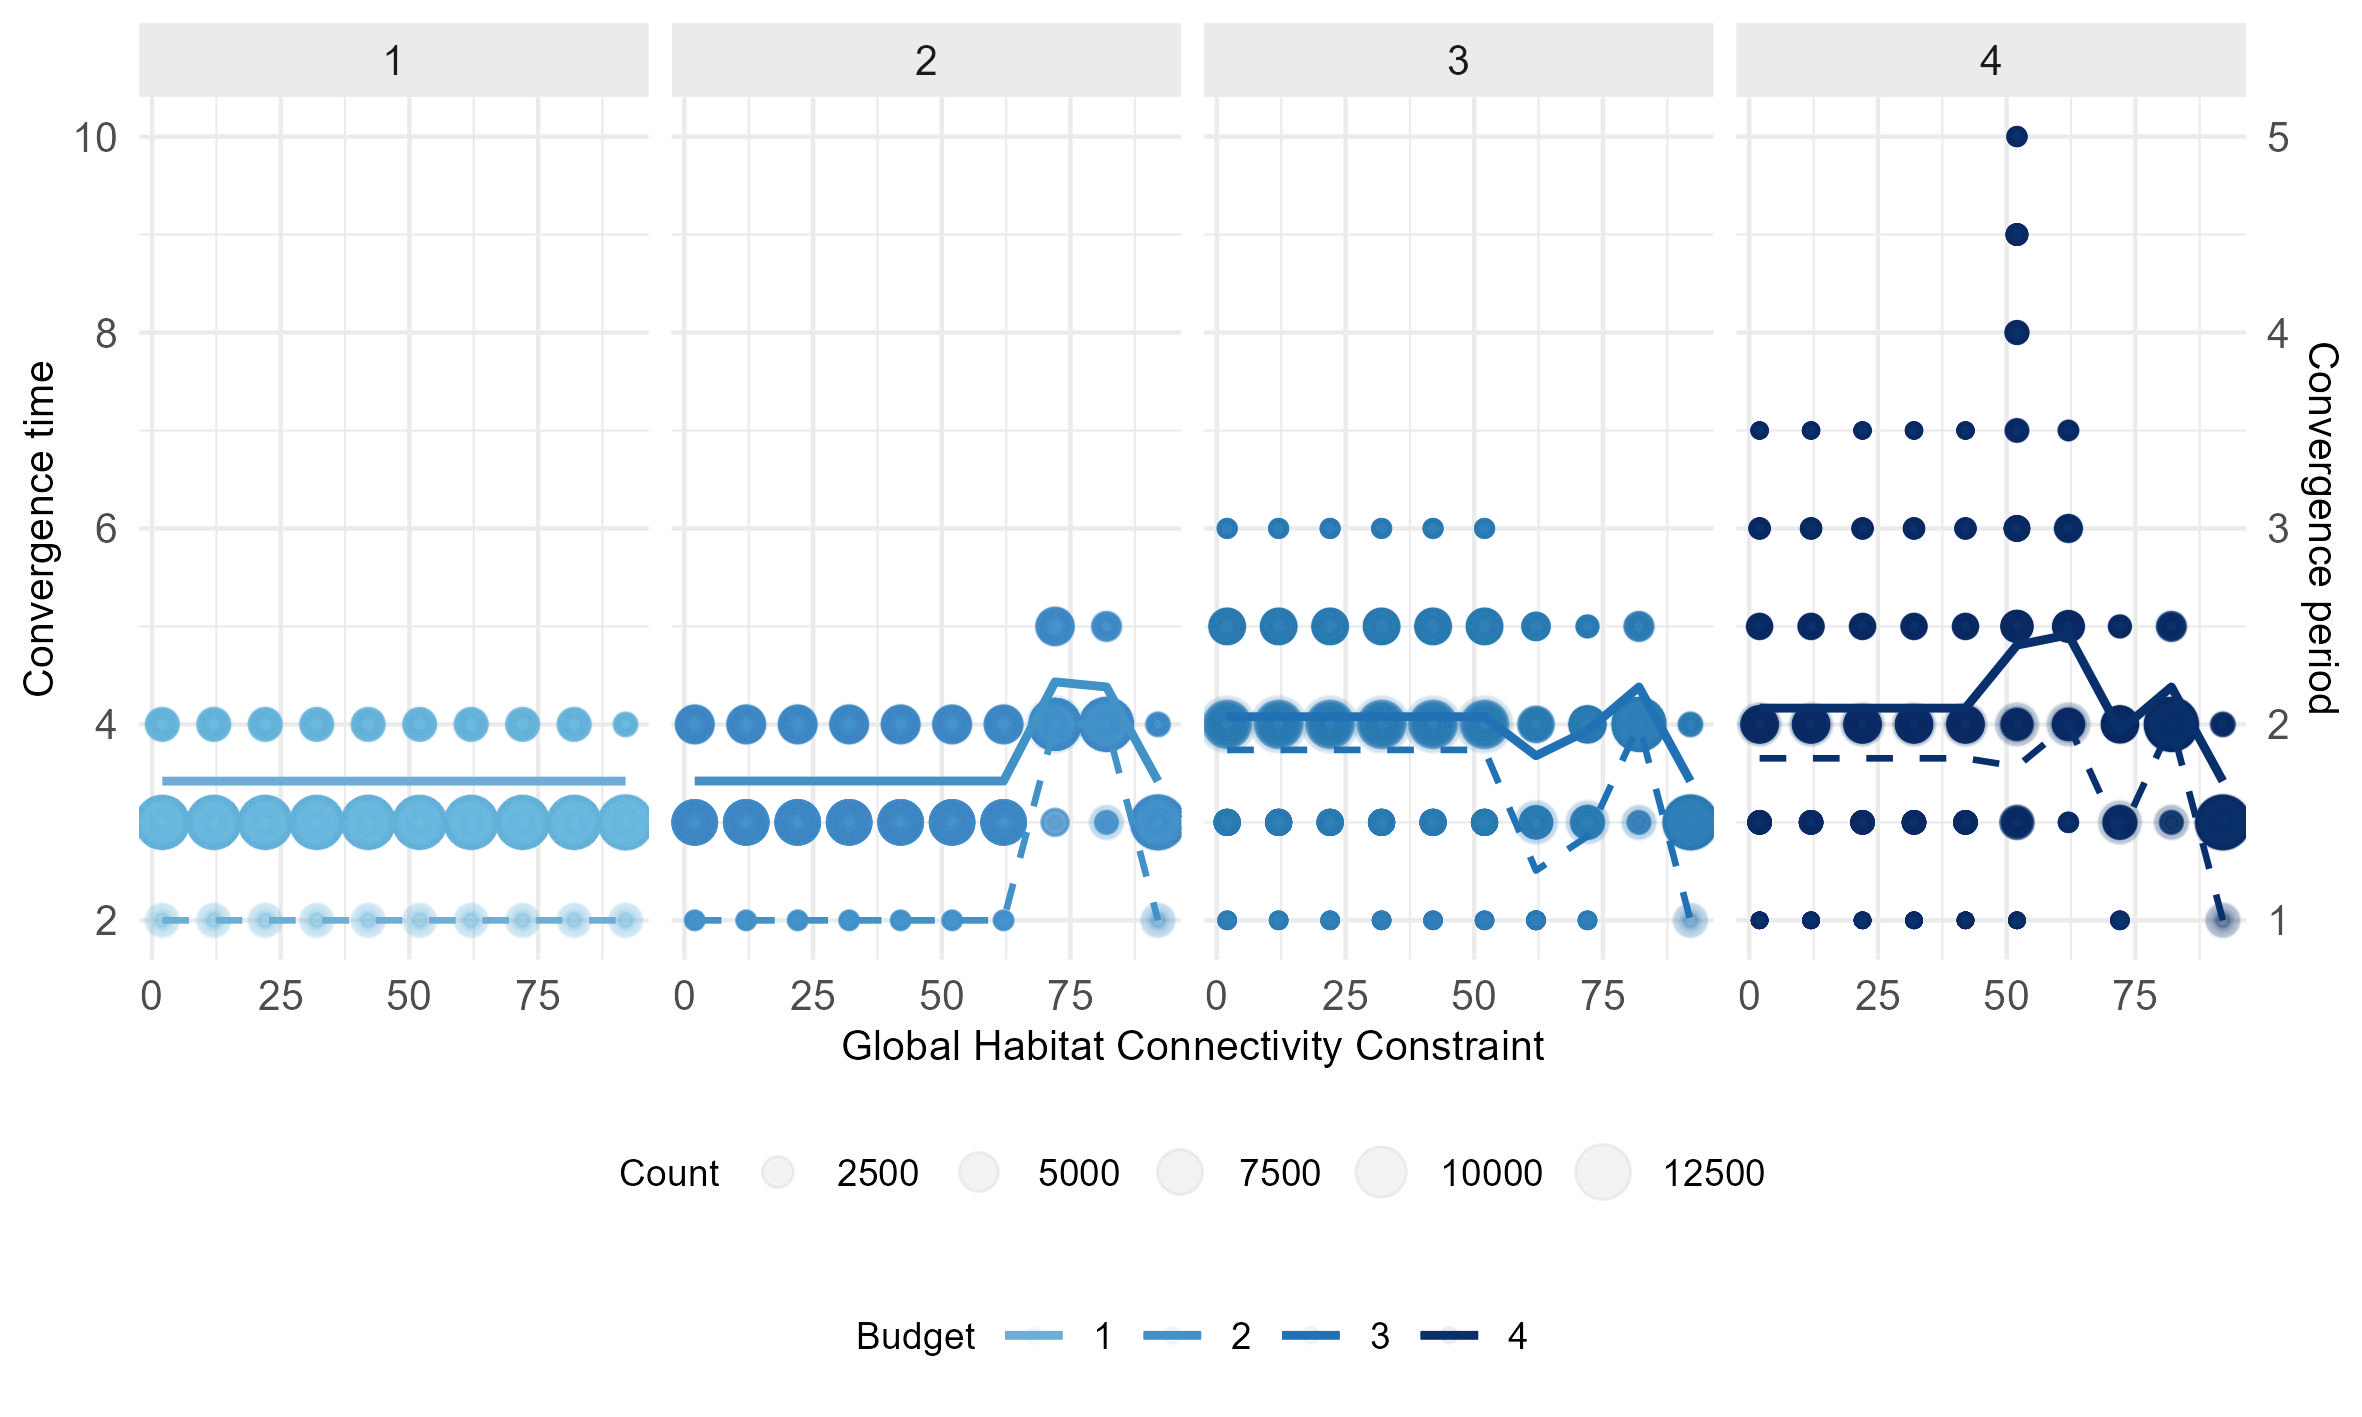
\includegraphics[width = .8\textwidth]{figures/wildland/convergence_times.jpg}
    		\caption{Convergence times and period across global habitat connectivity and budget constraints}
    		\caption*{Average convergence time is displayed with full lines and measured on the left $y$-axis, while average convergence period is displayed with dashed lines and measured on the left $y$-axis} 
    		\label{fig:convergence_time}
	\end{subfigure}
	\begin{subfigure}[b]{\textwidth}
    		\centering
    		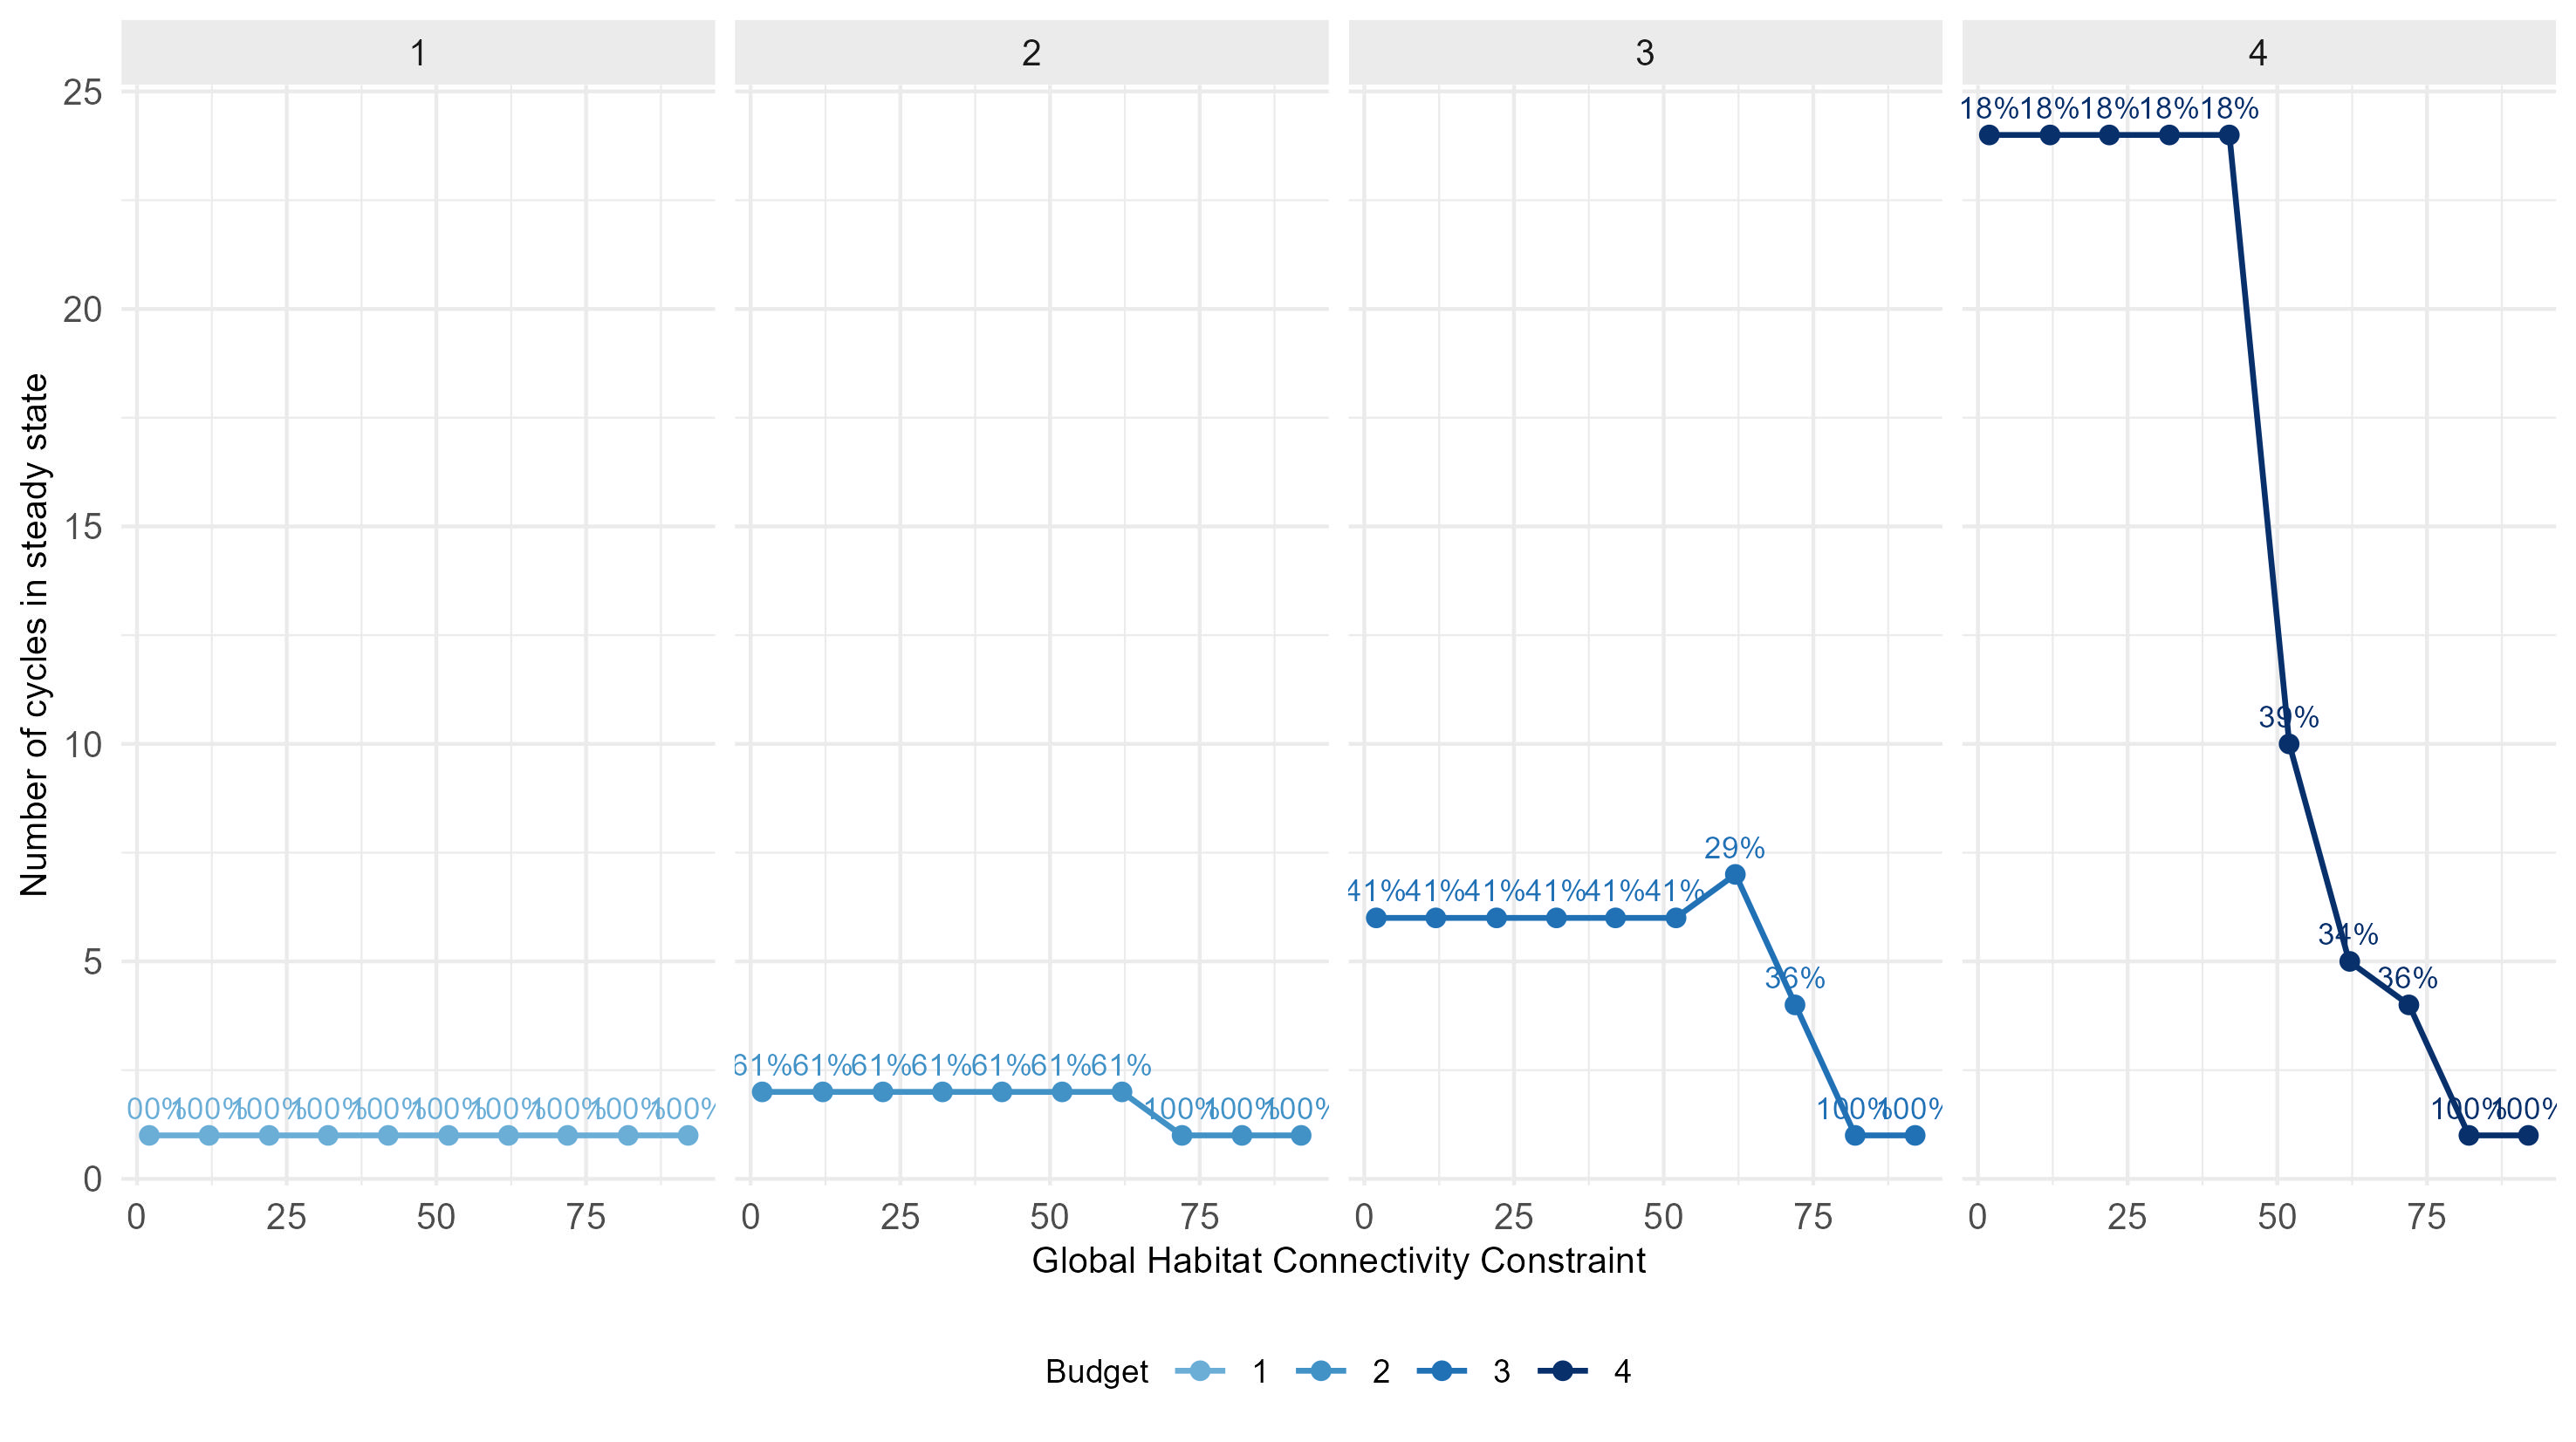
\includegraphics[width = .8\textwidth]{figures/wildland/number_of_cycles.jpg}
    		\caption{Number of cycles in steady state as the global habitat connectivity constraint evolves and across budget constraints}
    		\caption*{Above each data point is the frequence of the most represented cycle in the data.} 
    		\label{fig:distrib_cycles}
	\end{subfigure}
\caption{Steady state cycles: convergence and distribution}
\end{figure}
%
Figure \ref{fig:distrib_cycles} shows that conditional on data availability on every patch, the more the decision maker wants to conserve biodiversity, the fewer steady-state landscapes she has to consider. An increase in the habitat requirement reduces the room for maneuver. Indeed, budget acts as a complexifying factor: the larger the budget (relative to costs), the larger the set of steady-states to consider. 
Aiming for relatively large habitat connectivity reduces the set of viable strategies to be considered and can more efficiently guide policy. 
%


\subsection{Properties of steady state landscapes: surface, fragmentation, and diversity}
\label{sec:landscape_char}

Figure \ref{fig:cycles} displays, for each global habitat connectivity and budget constraint levels, the most frequent steady-state cycle.
%Figures \ref{fig:indicators_1} and \ref{fig:indicators_2} show the indicators (detailed in section \ref{section:indicators}) averaged over all the steady-state landscape cycles. 
Figure \ref{fig:indicators1} shows the indicators relative to the surface and components of the high-risk graph and figure \ref{fig:indicators2} shows the indicators related to diversity, both for landscapes of size $n=3$ and $4$, averaged over all the steady-state landscape cycles. 


\begin{figure}[H]
    \centering
    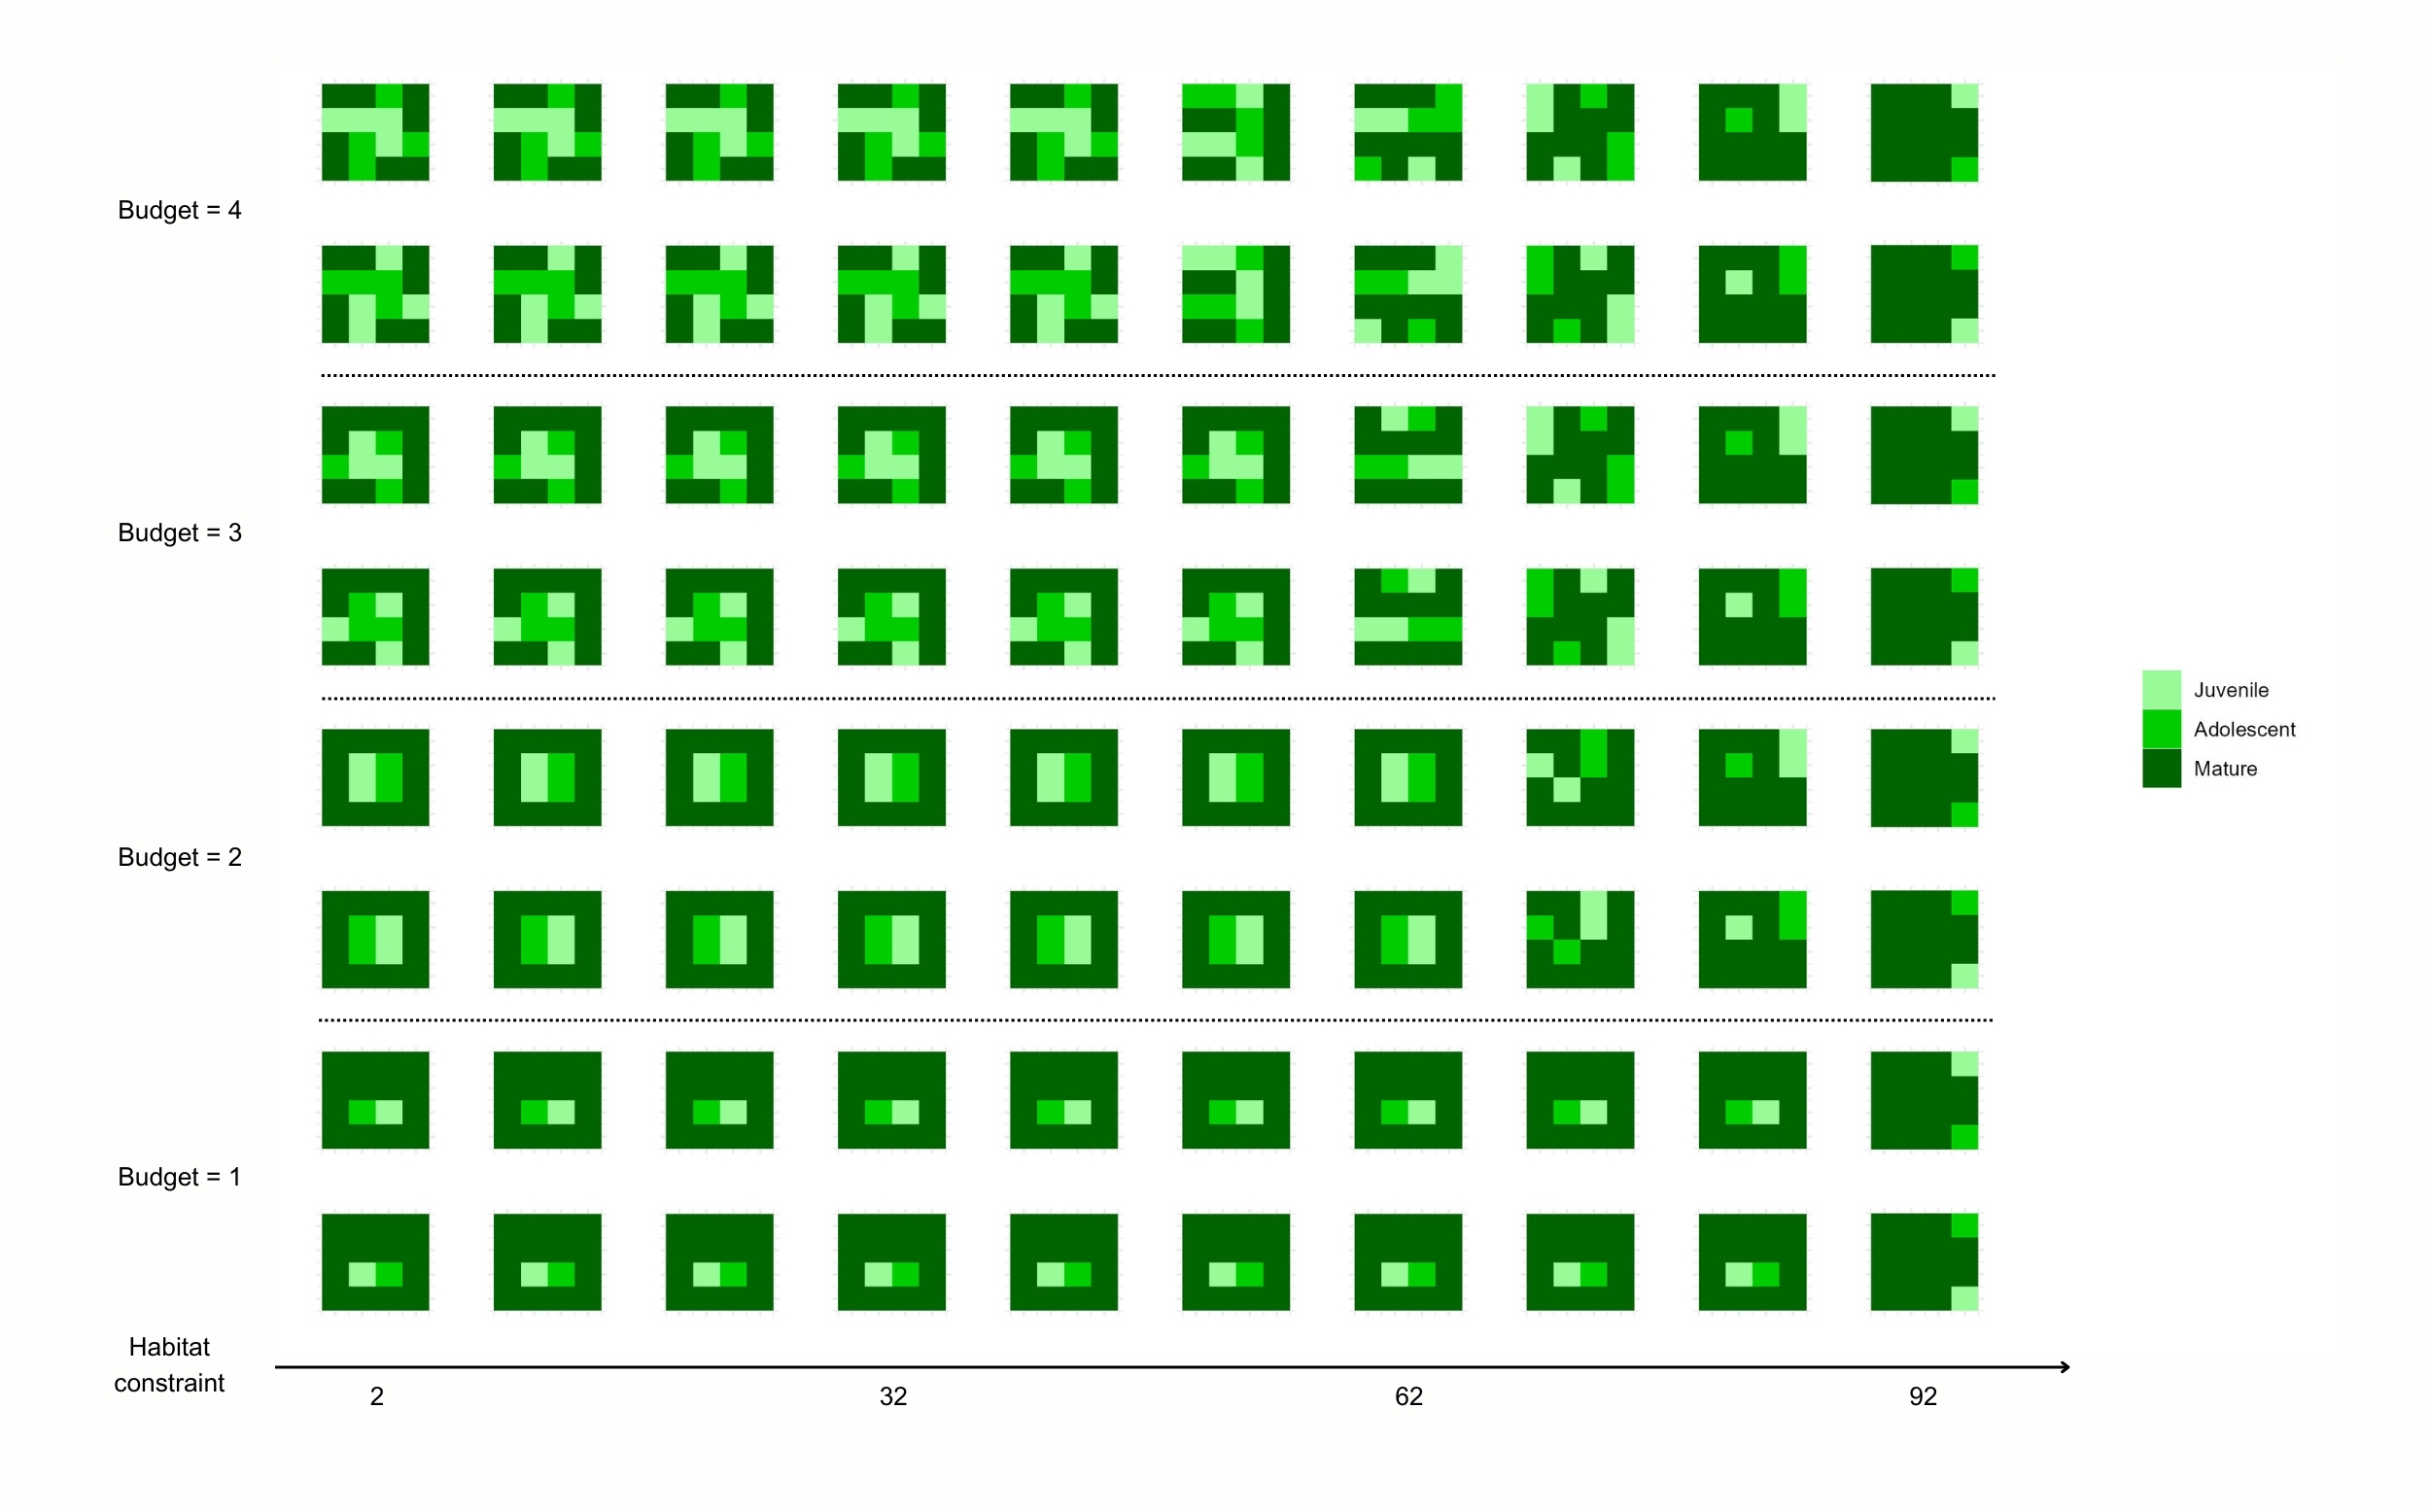
\includegraphics[width=\textwidth]{figures/wildland/full_cycle_canva.jpg}
    \caption{Most represented cycles for each global habitat and budget  constraint levels}
    \label{fig:cycles}
\end{figure}


\begin{figure}
    \centering
    \begin{subfigure}[b]{.48\textwidth}
        \centering
        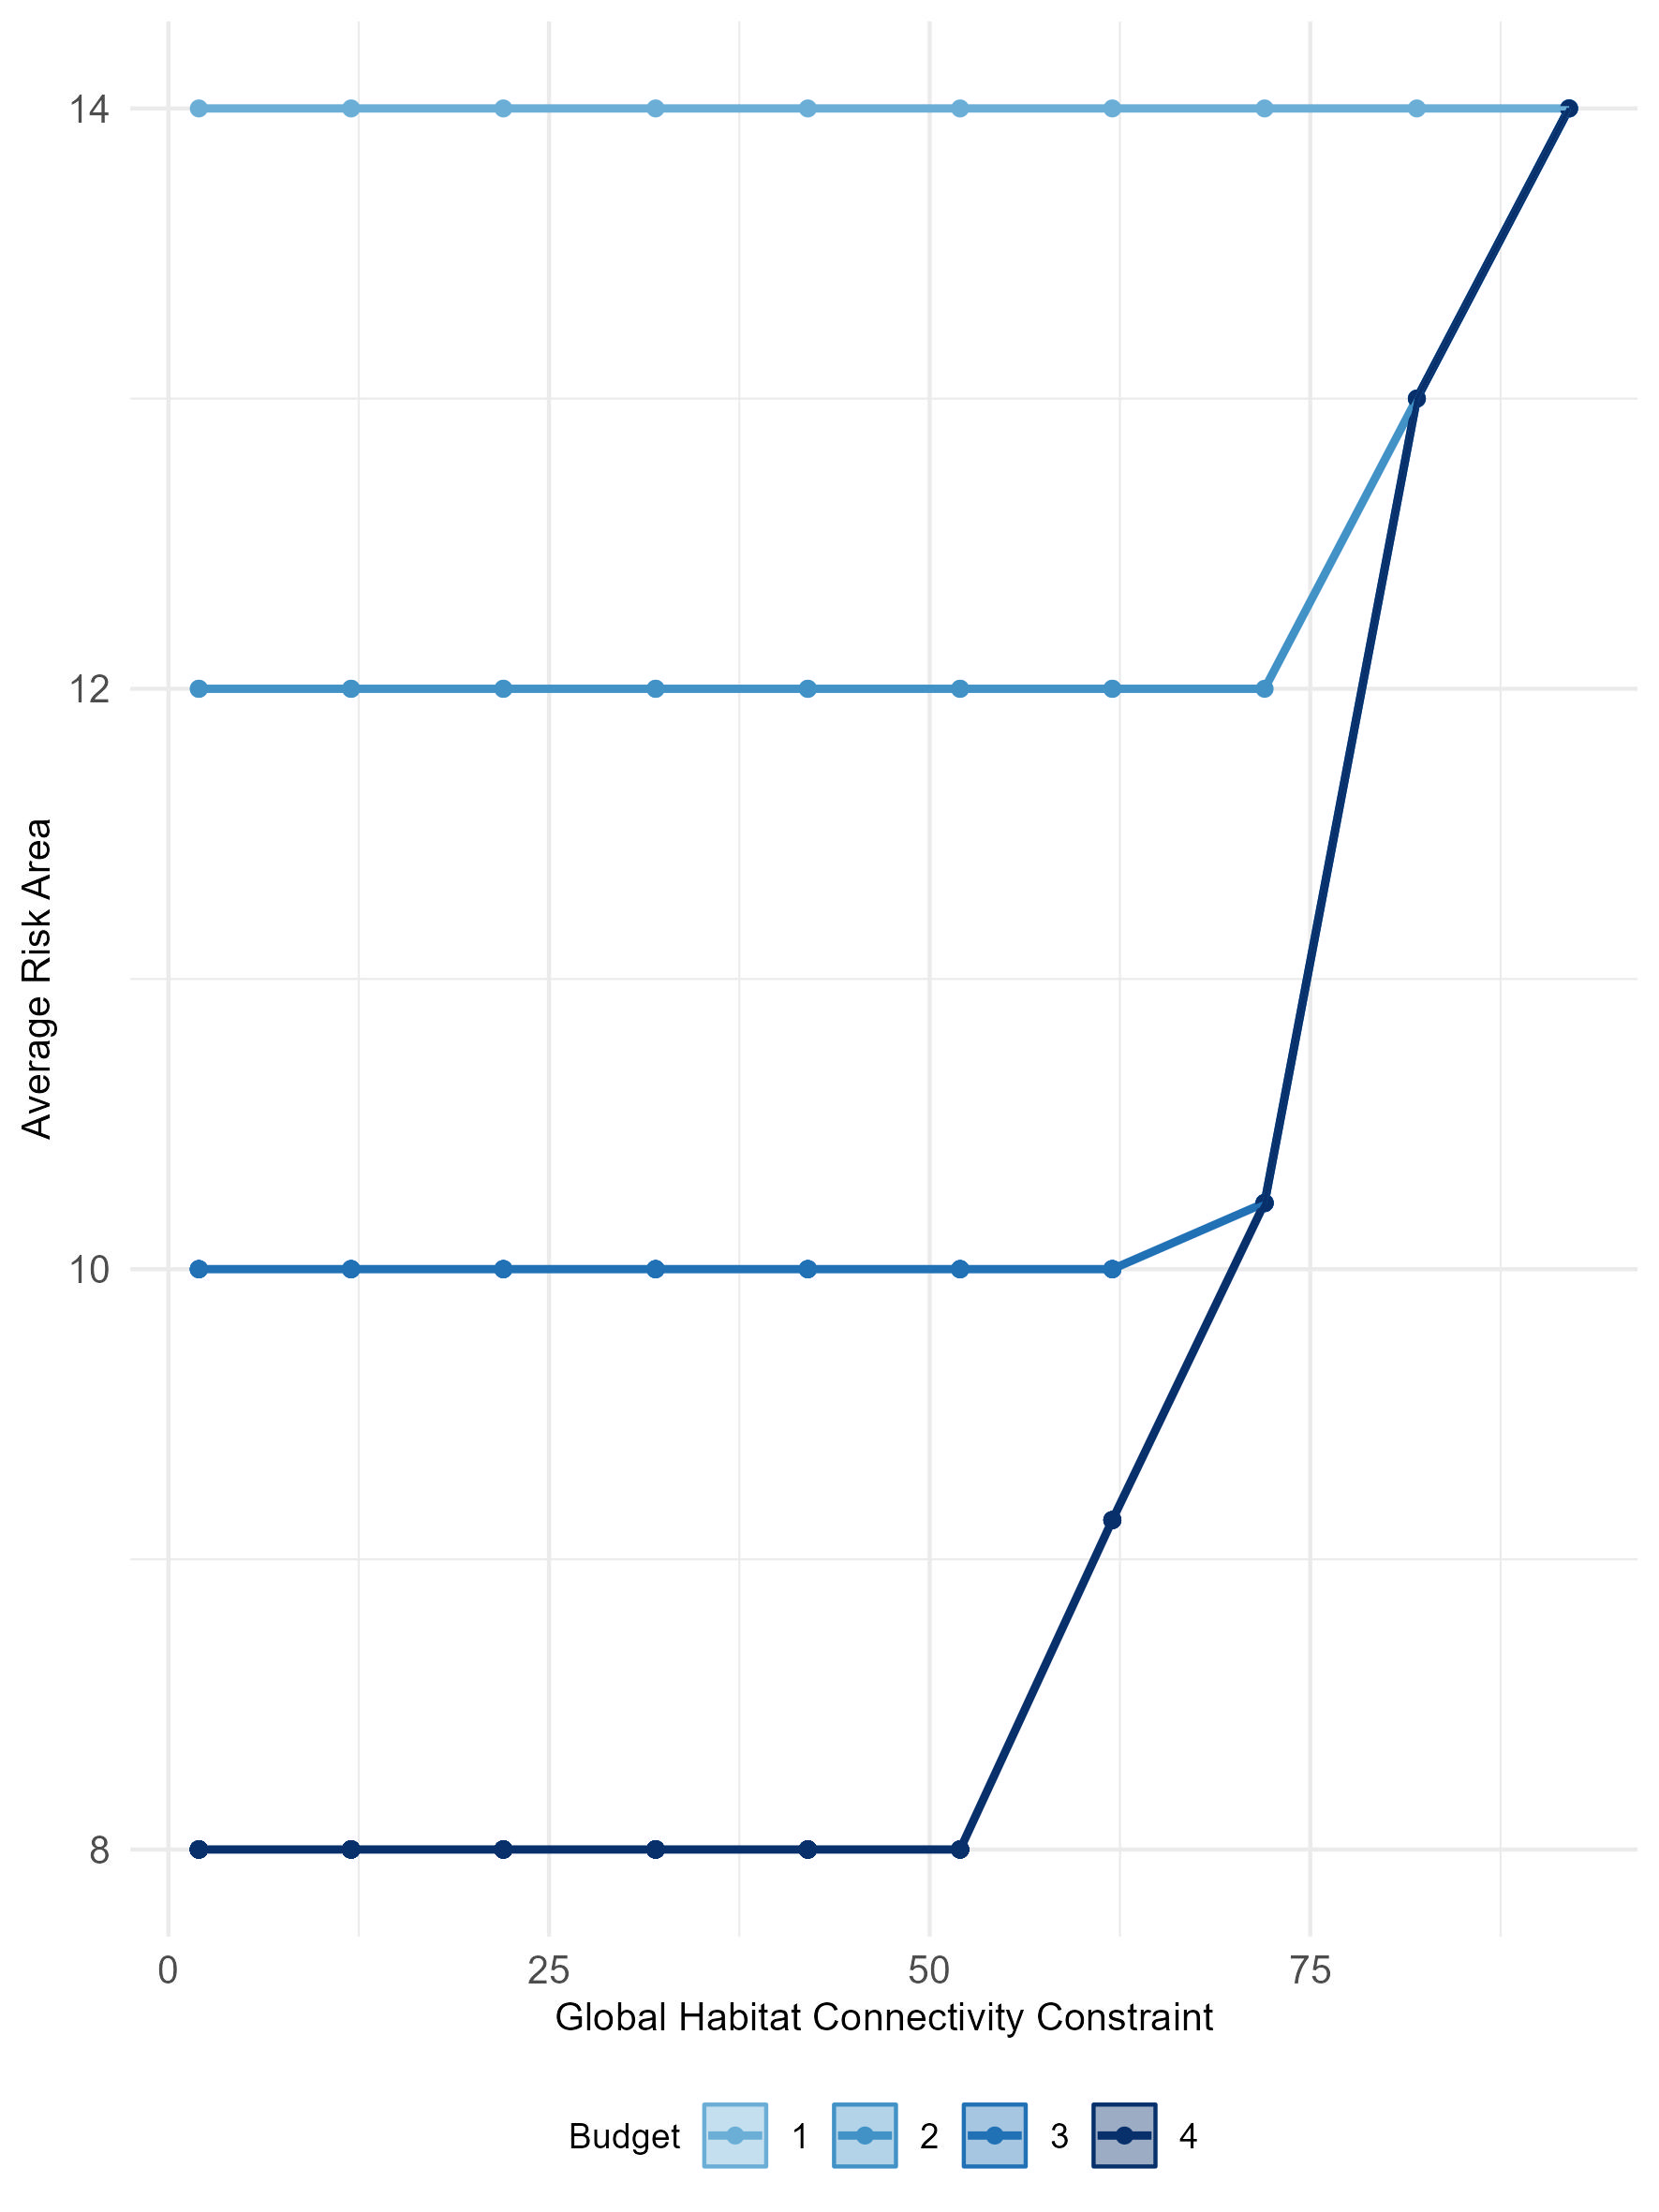
\includegraphics[height = .4\textheight]{figures/wildland/average_areaF.jpg}
        \caption{Average area}
        \label{fig:area}
    \end{subfigure}
    \hfill
    \begin{subfigure}[b]{.48\textwidth}
        \centering
        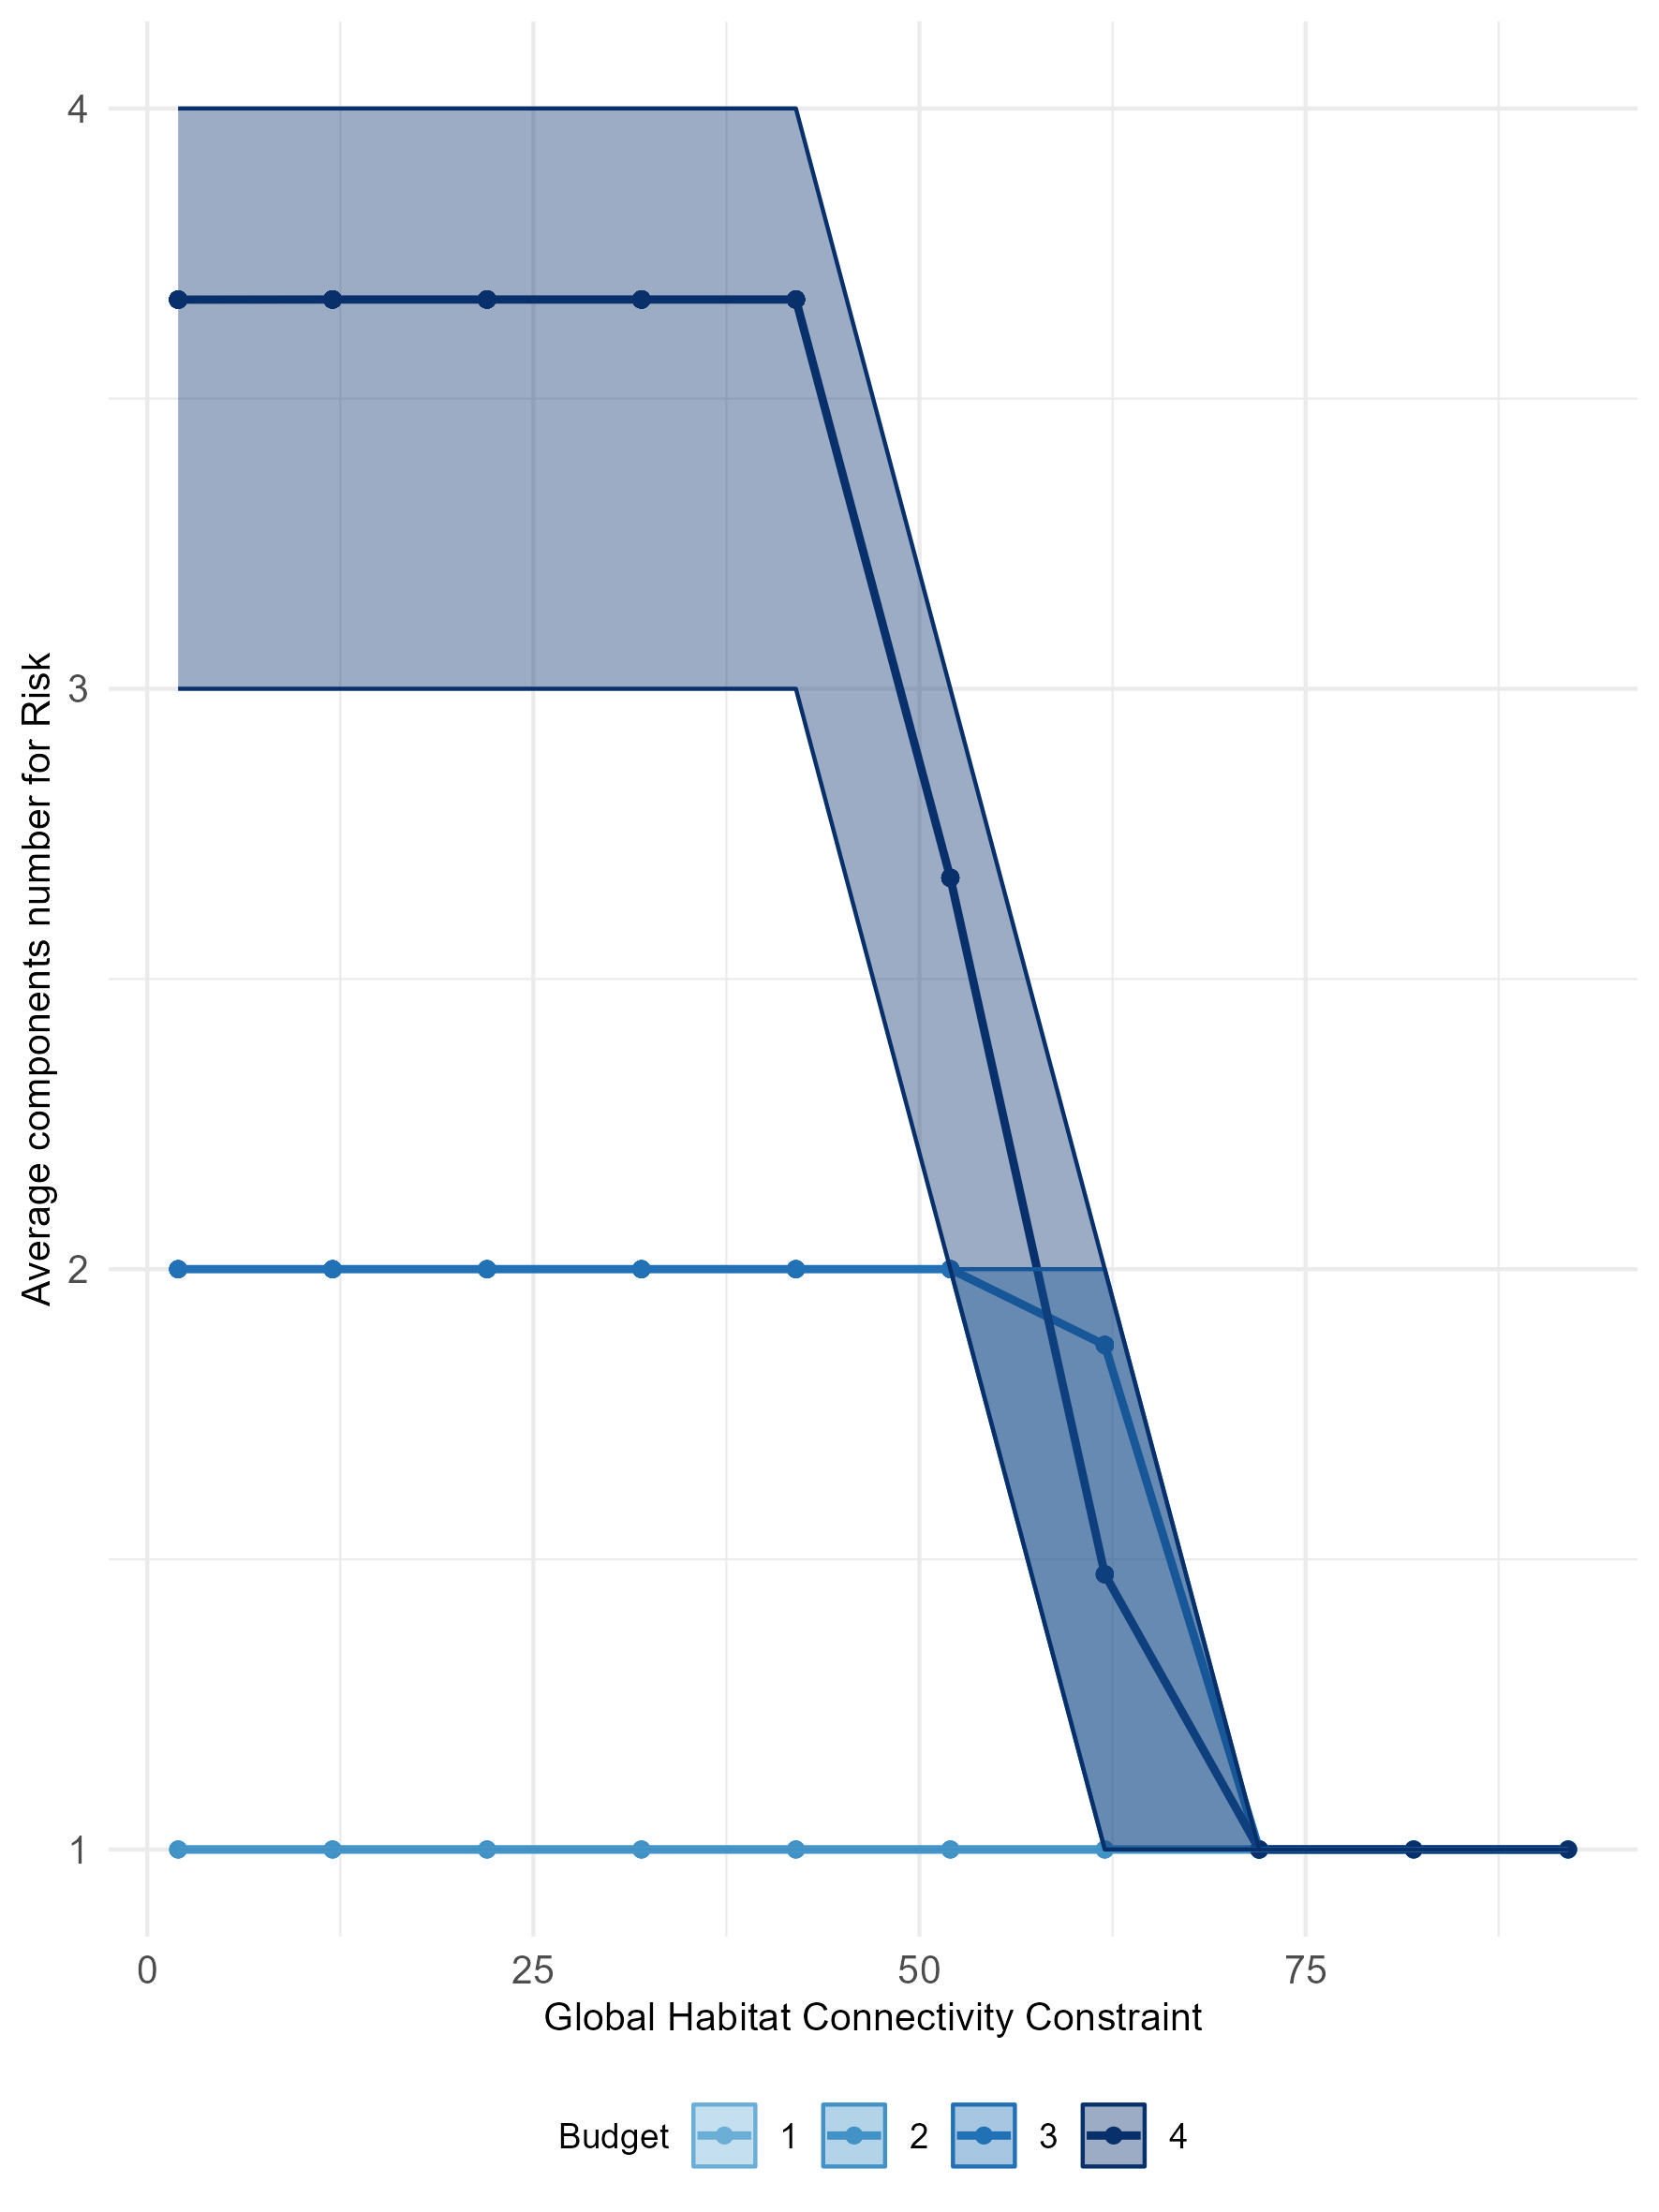
\includegraphics[height = .4\textheight]{figures/wildland/average_components_number.jpg}
        \caption{Average component number}
        \label{fig:component_number}
    \end{subfigure}
    
    \vspace{1em} % Add some vertical space between the rows

    \begin{subfigure}[b]{.48\textwidth}
        \centering
        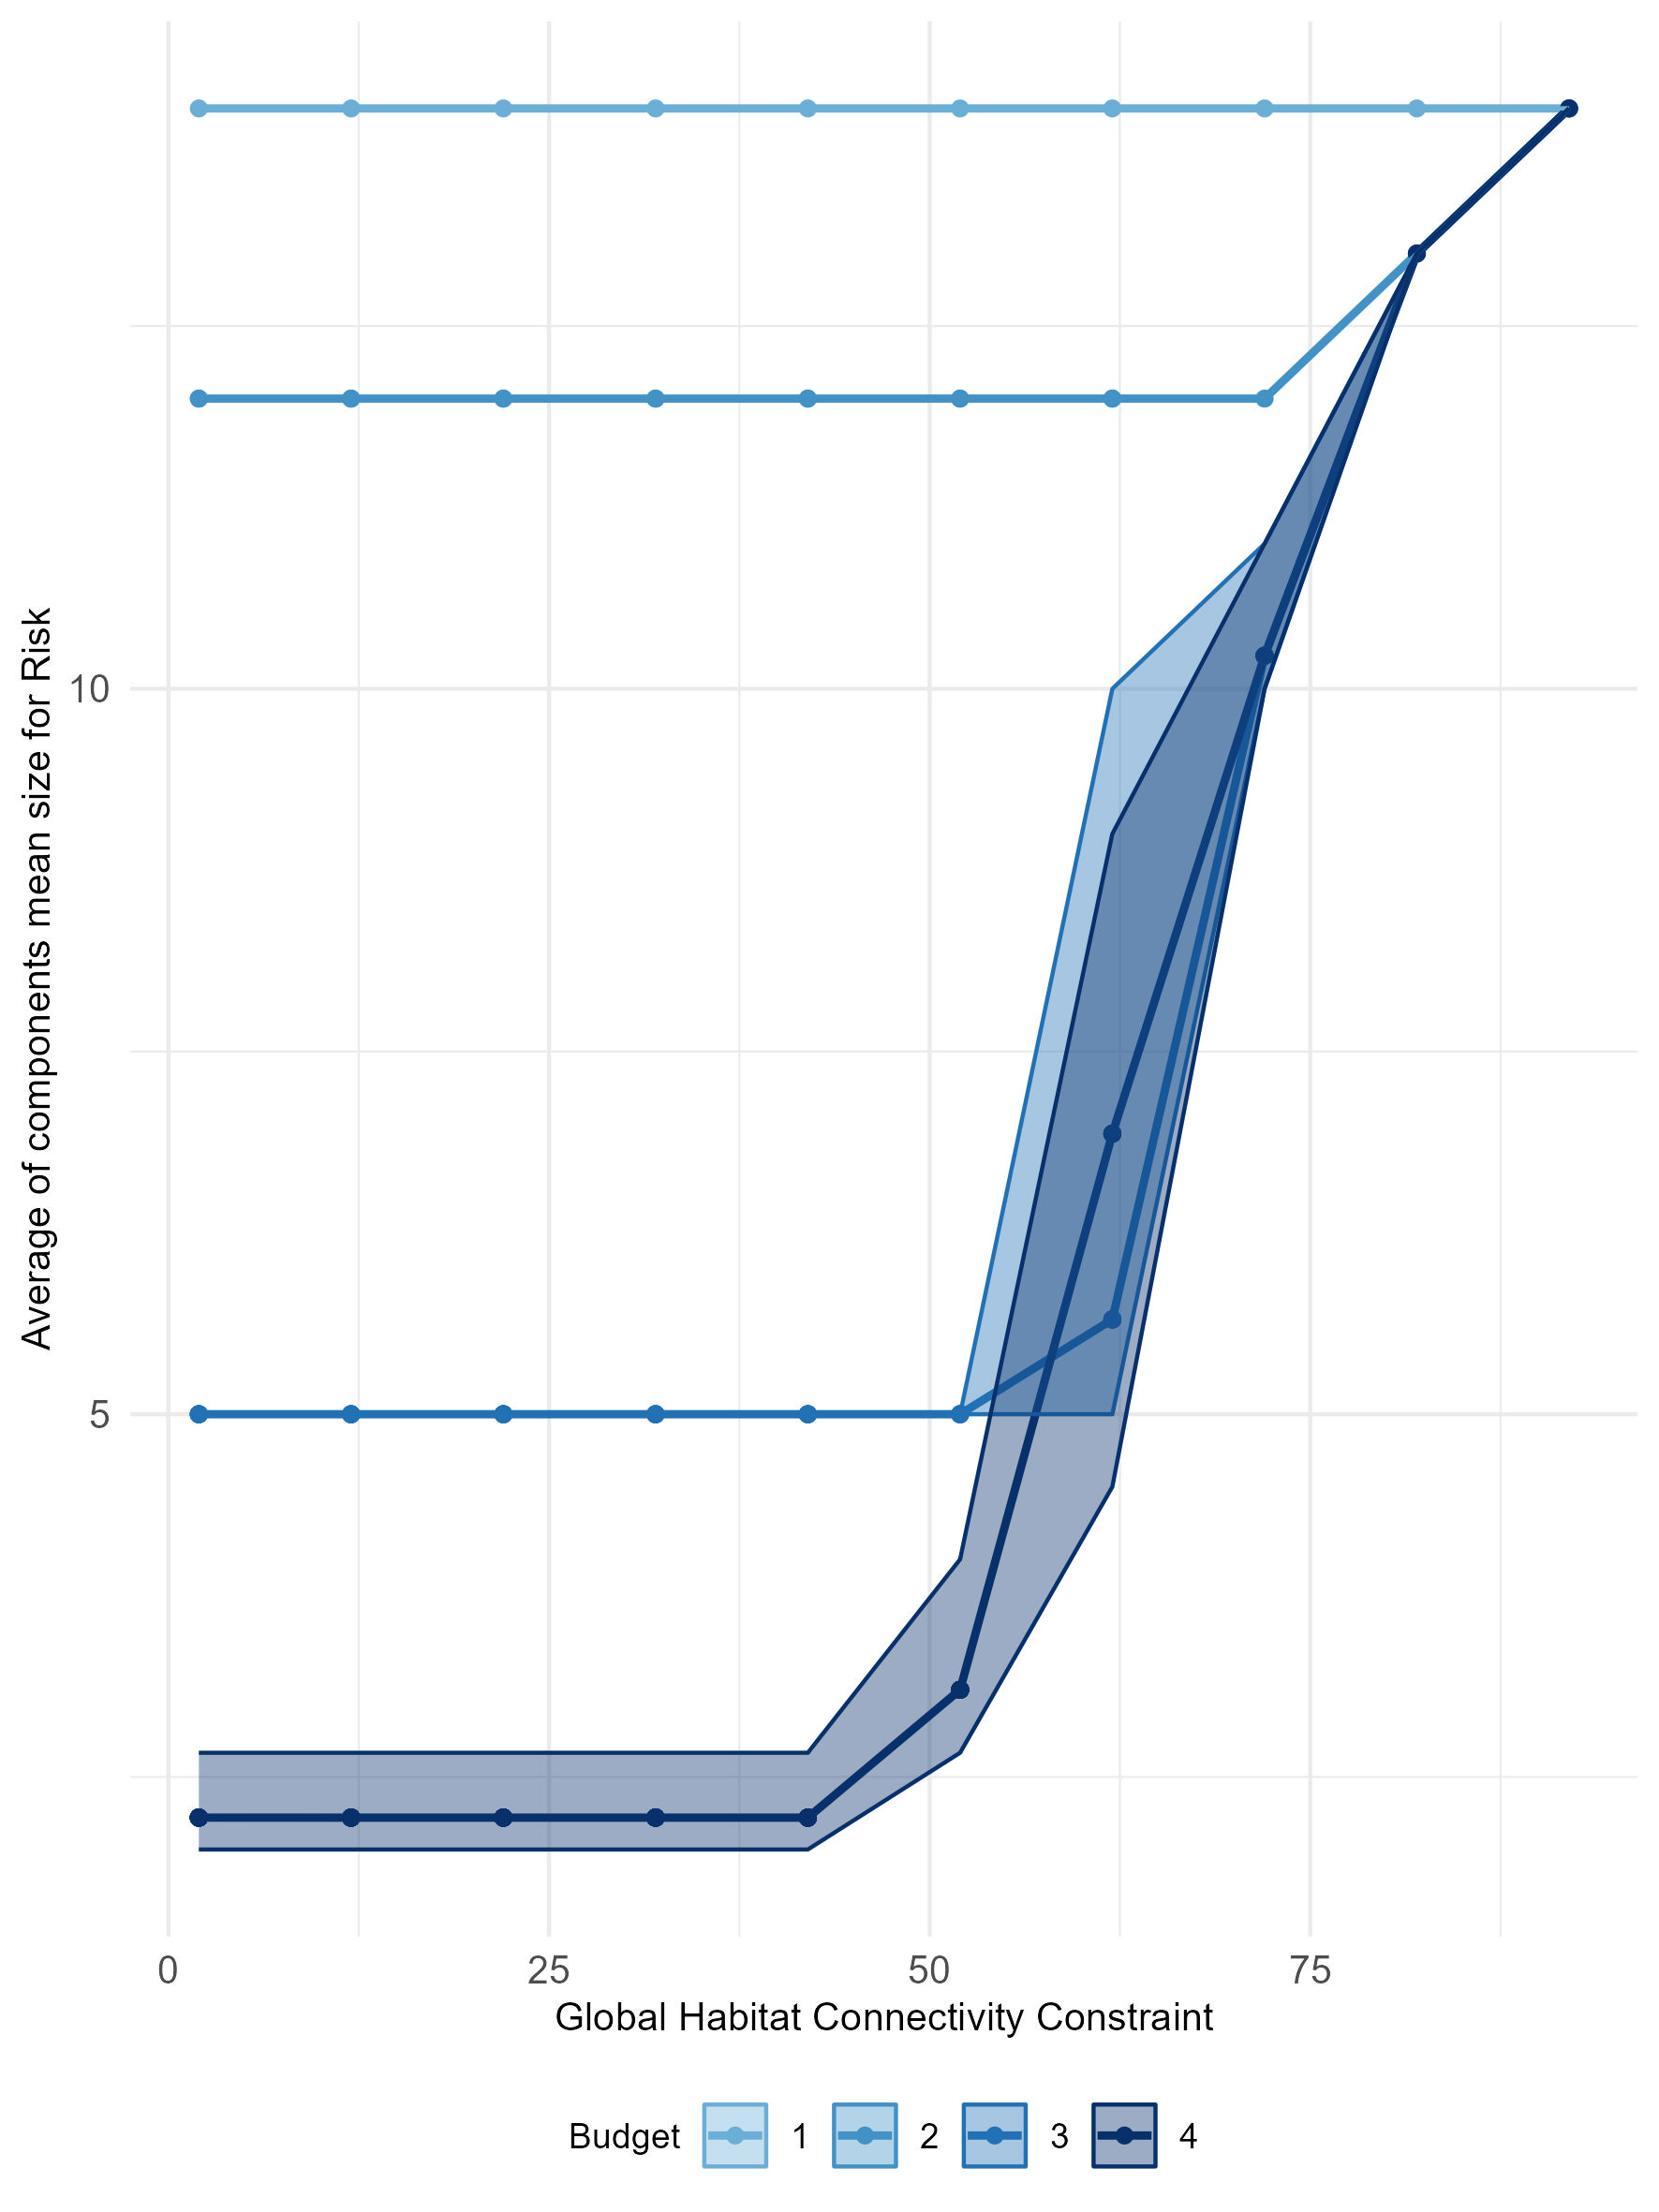
\includegraphics[height = .4\textheight]{figures/wildland/average_components_mean_size.jpg}
        \caption{Average components size}
        \label{fig:components_size}
    \end{subfigure}
    
    \caption{Indicators relative to surface and components across habitat and budget constraints}
    \caption*{The indicators are averaged across the cycles represented for each habitat and budget constraint levels.}
    \label{fig:indicators1}
\end{figure}


\begin{figure}
    \centering
    \begin{subfigure}[b]{.48\textwidth}
        \centering
        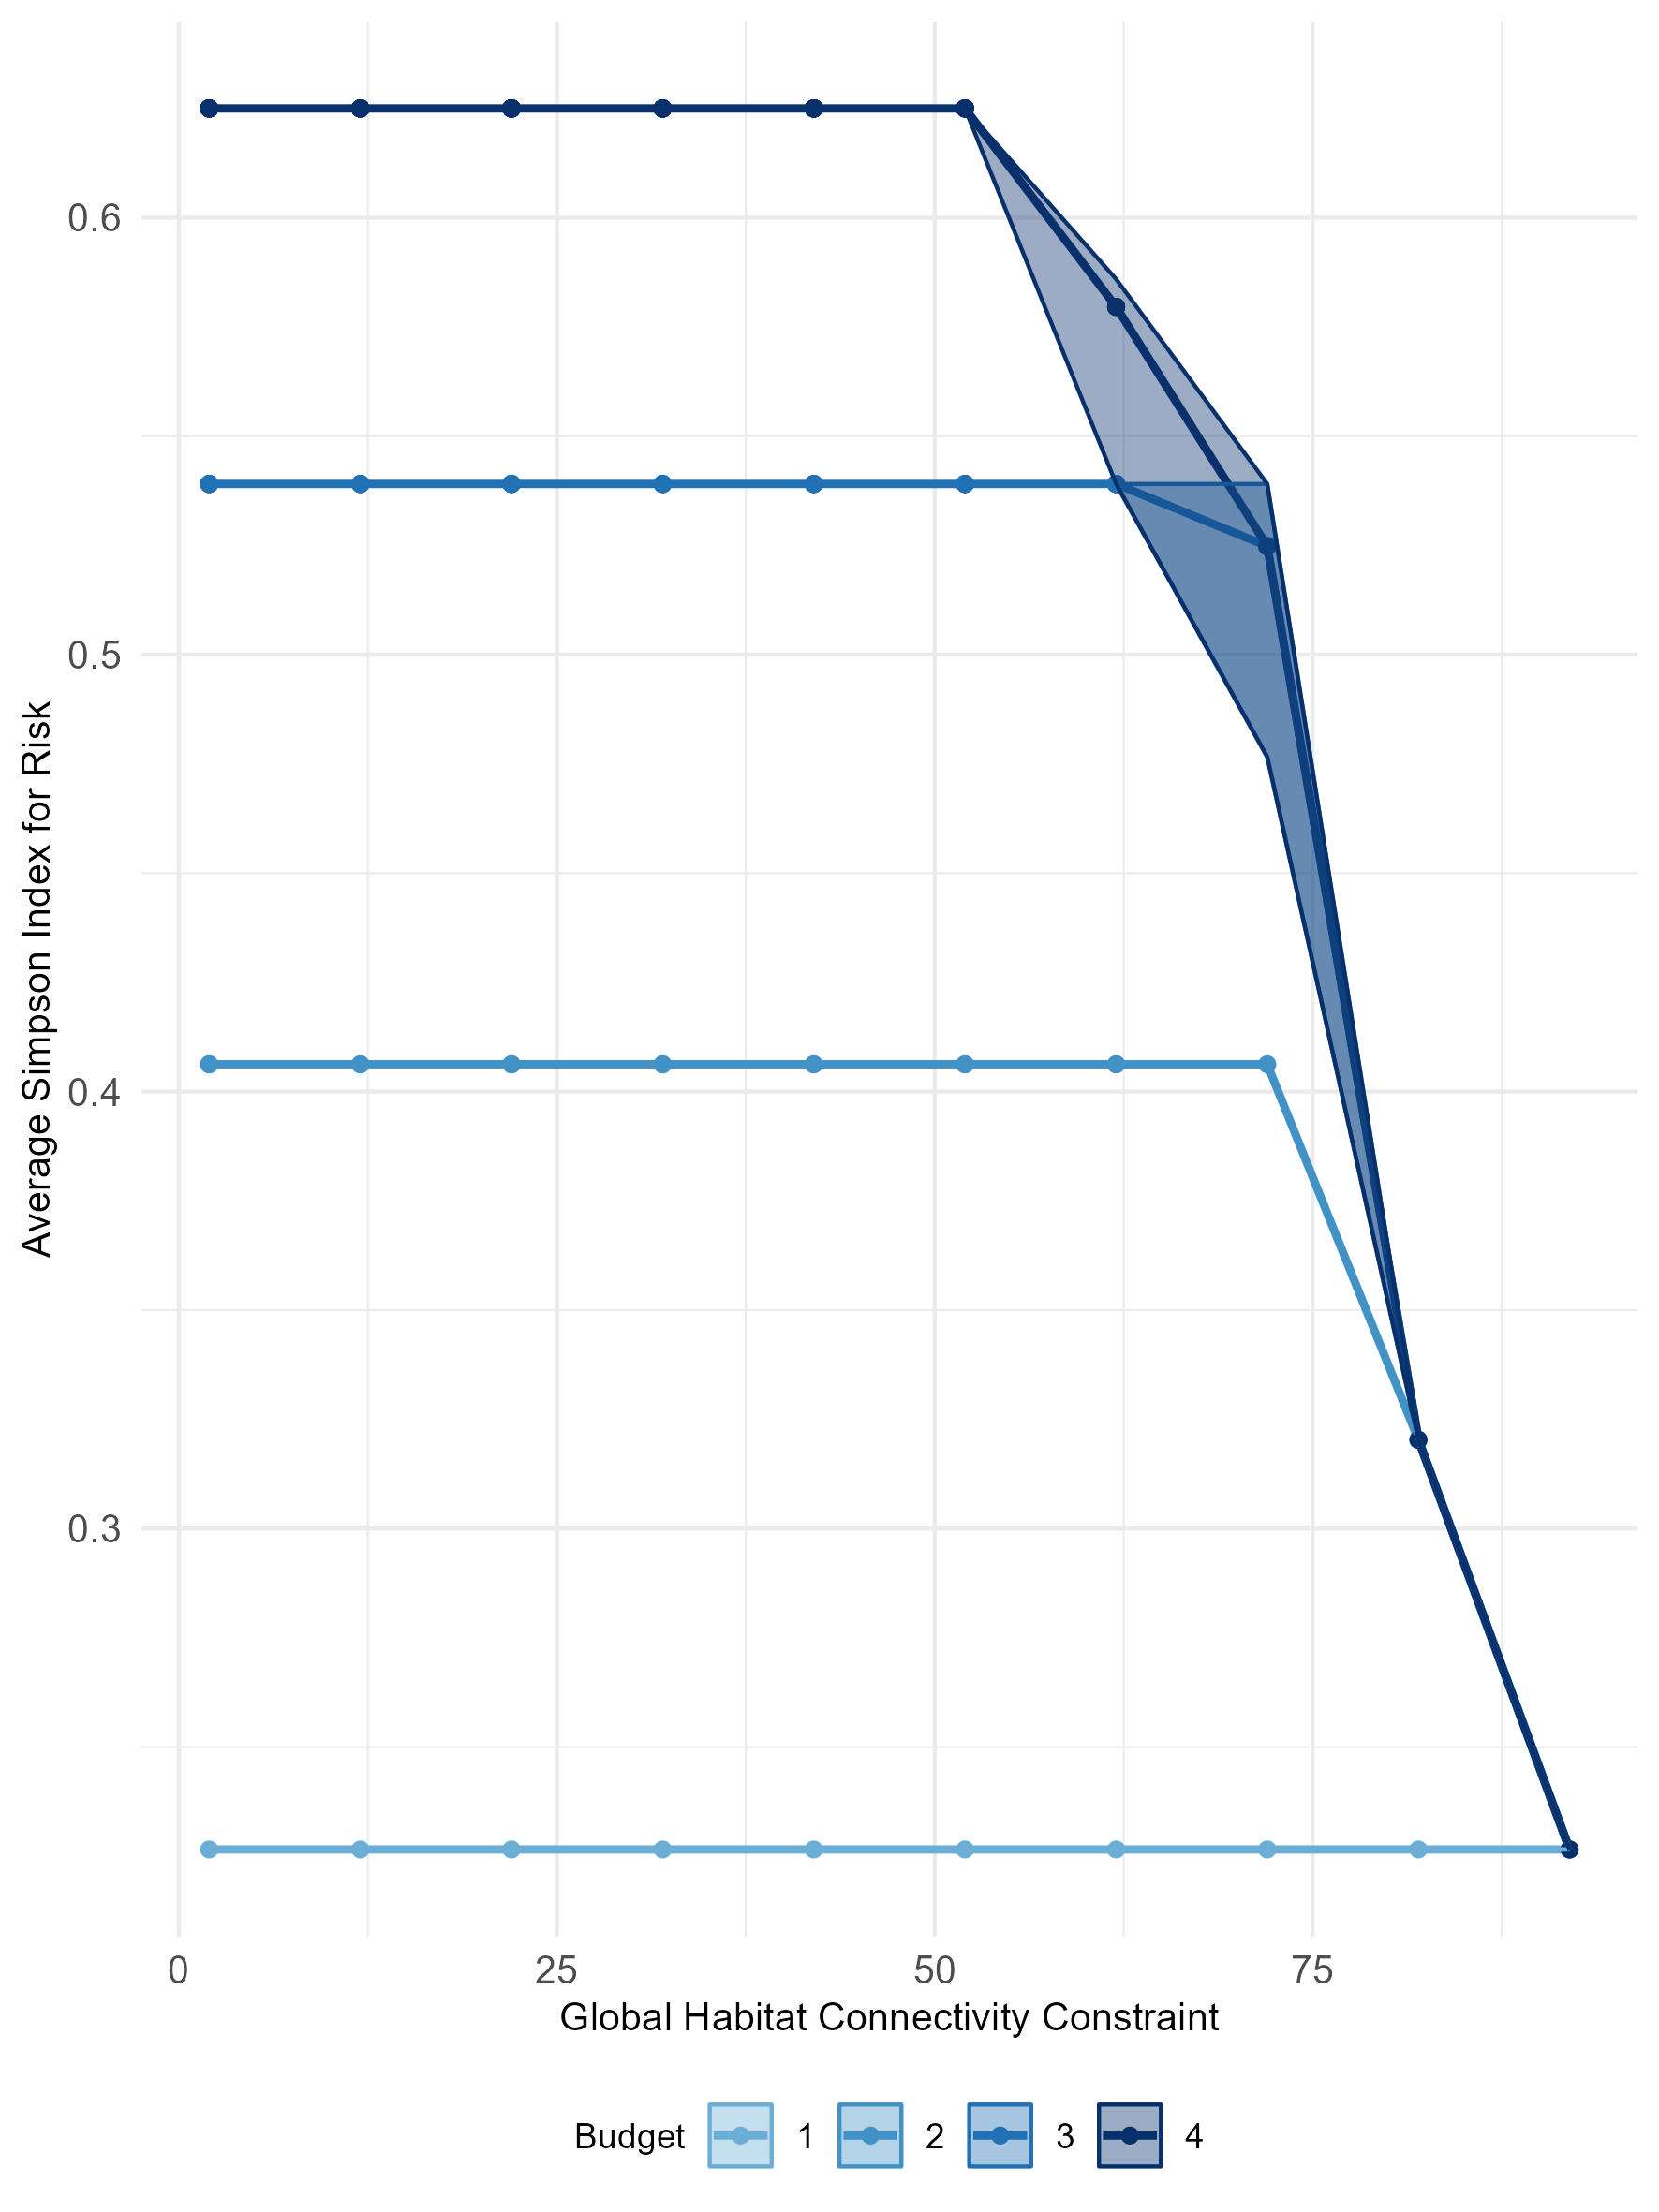
\includegraphics[height = .3\textheight]{figures/wildland/average_simpson.jpg}
        \caption{Average Simpson Index}
        \label{fig:simpson}
    \end{subfigure}
    \hfill
    \begin{subfigure}[b]{.48\textwidth}
        \centering
        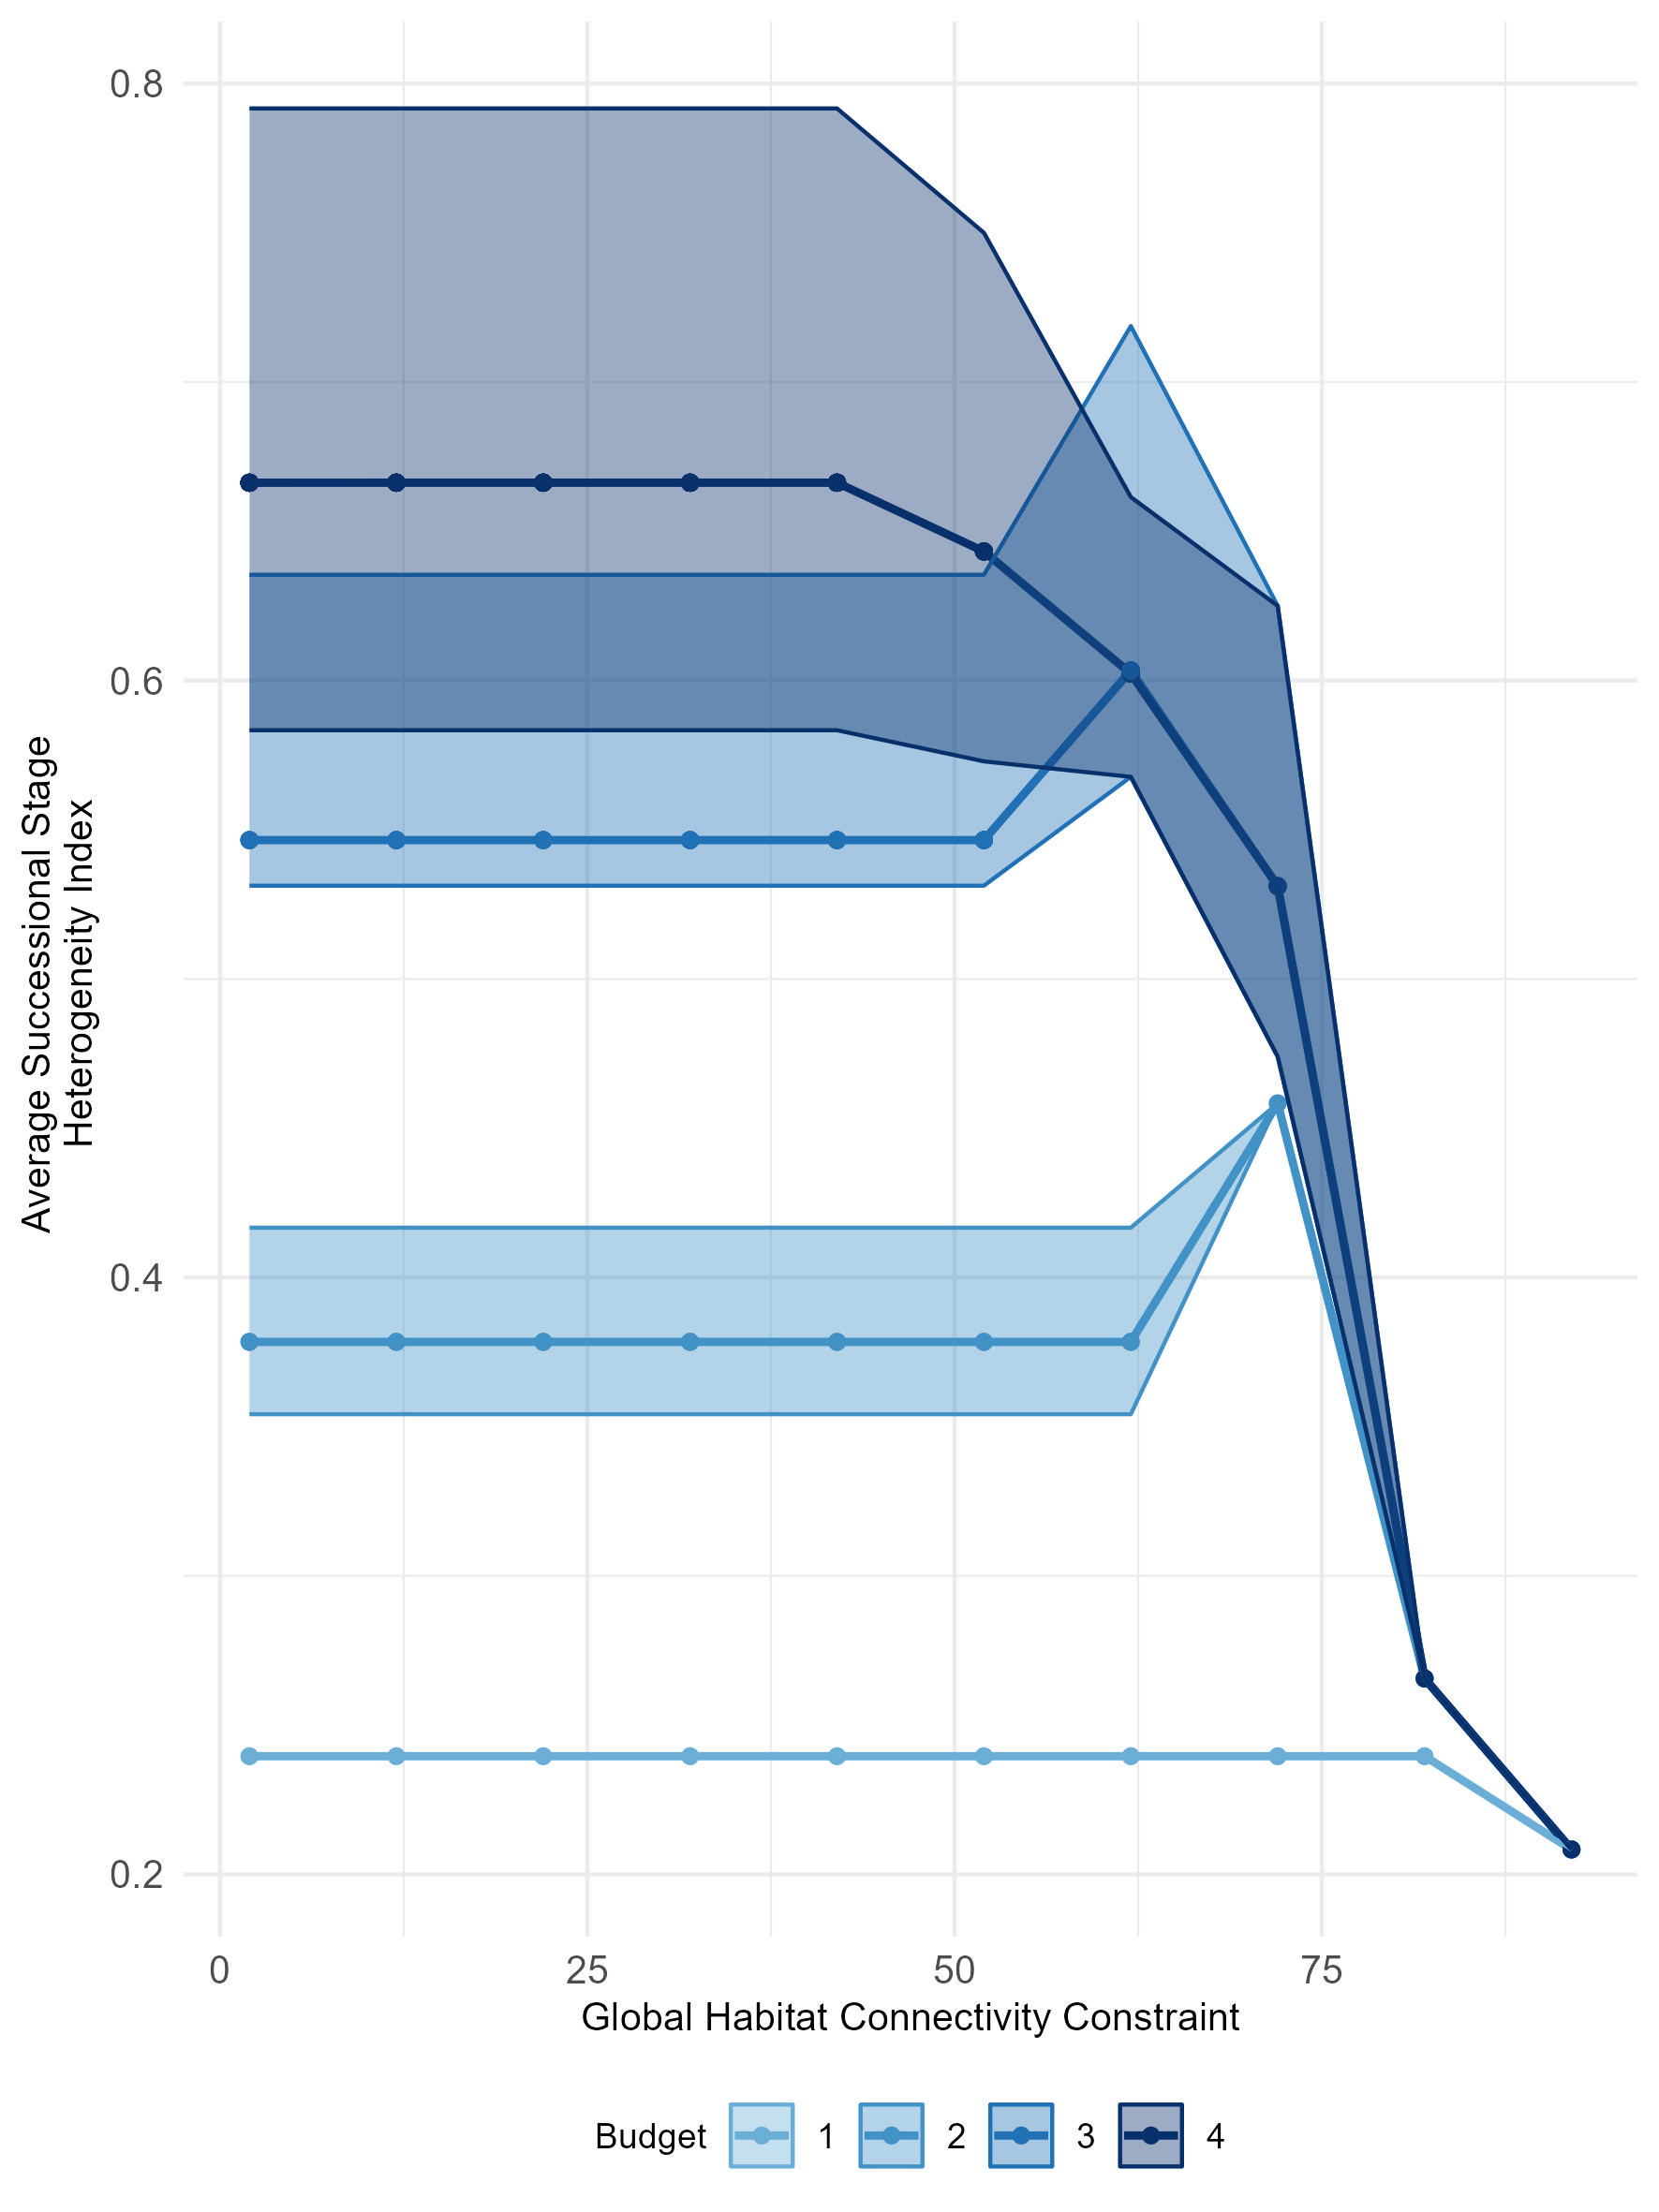
\includegraphics[height = .3\textheight]{figures/wildland/average_het.jpg}
        \caption{Average Successional Stage Heterogeneity Index}
        \label{fig:het}
    \end{subfigure}
       \vspace{1em} % Add some vertical space between the rows 
    \begin{subfigure}[b]{.48\textwidth}
        \centering
        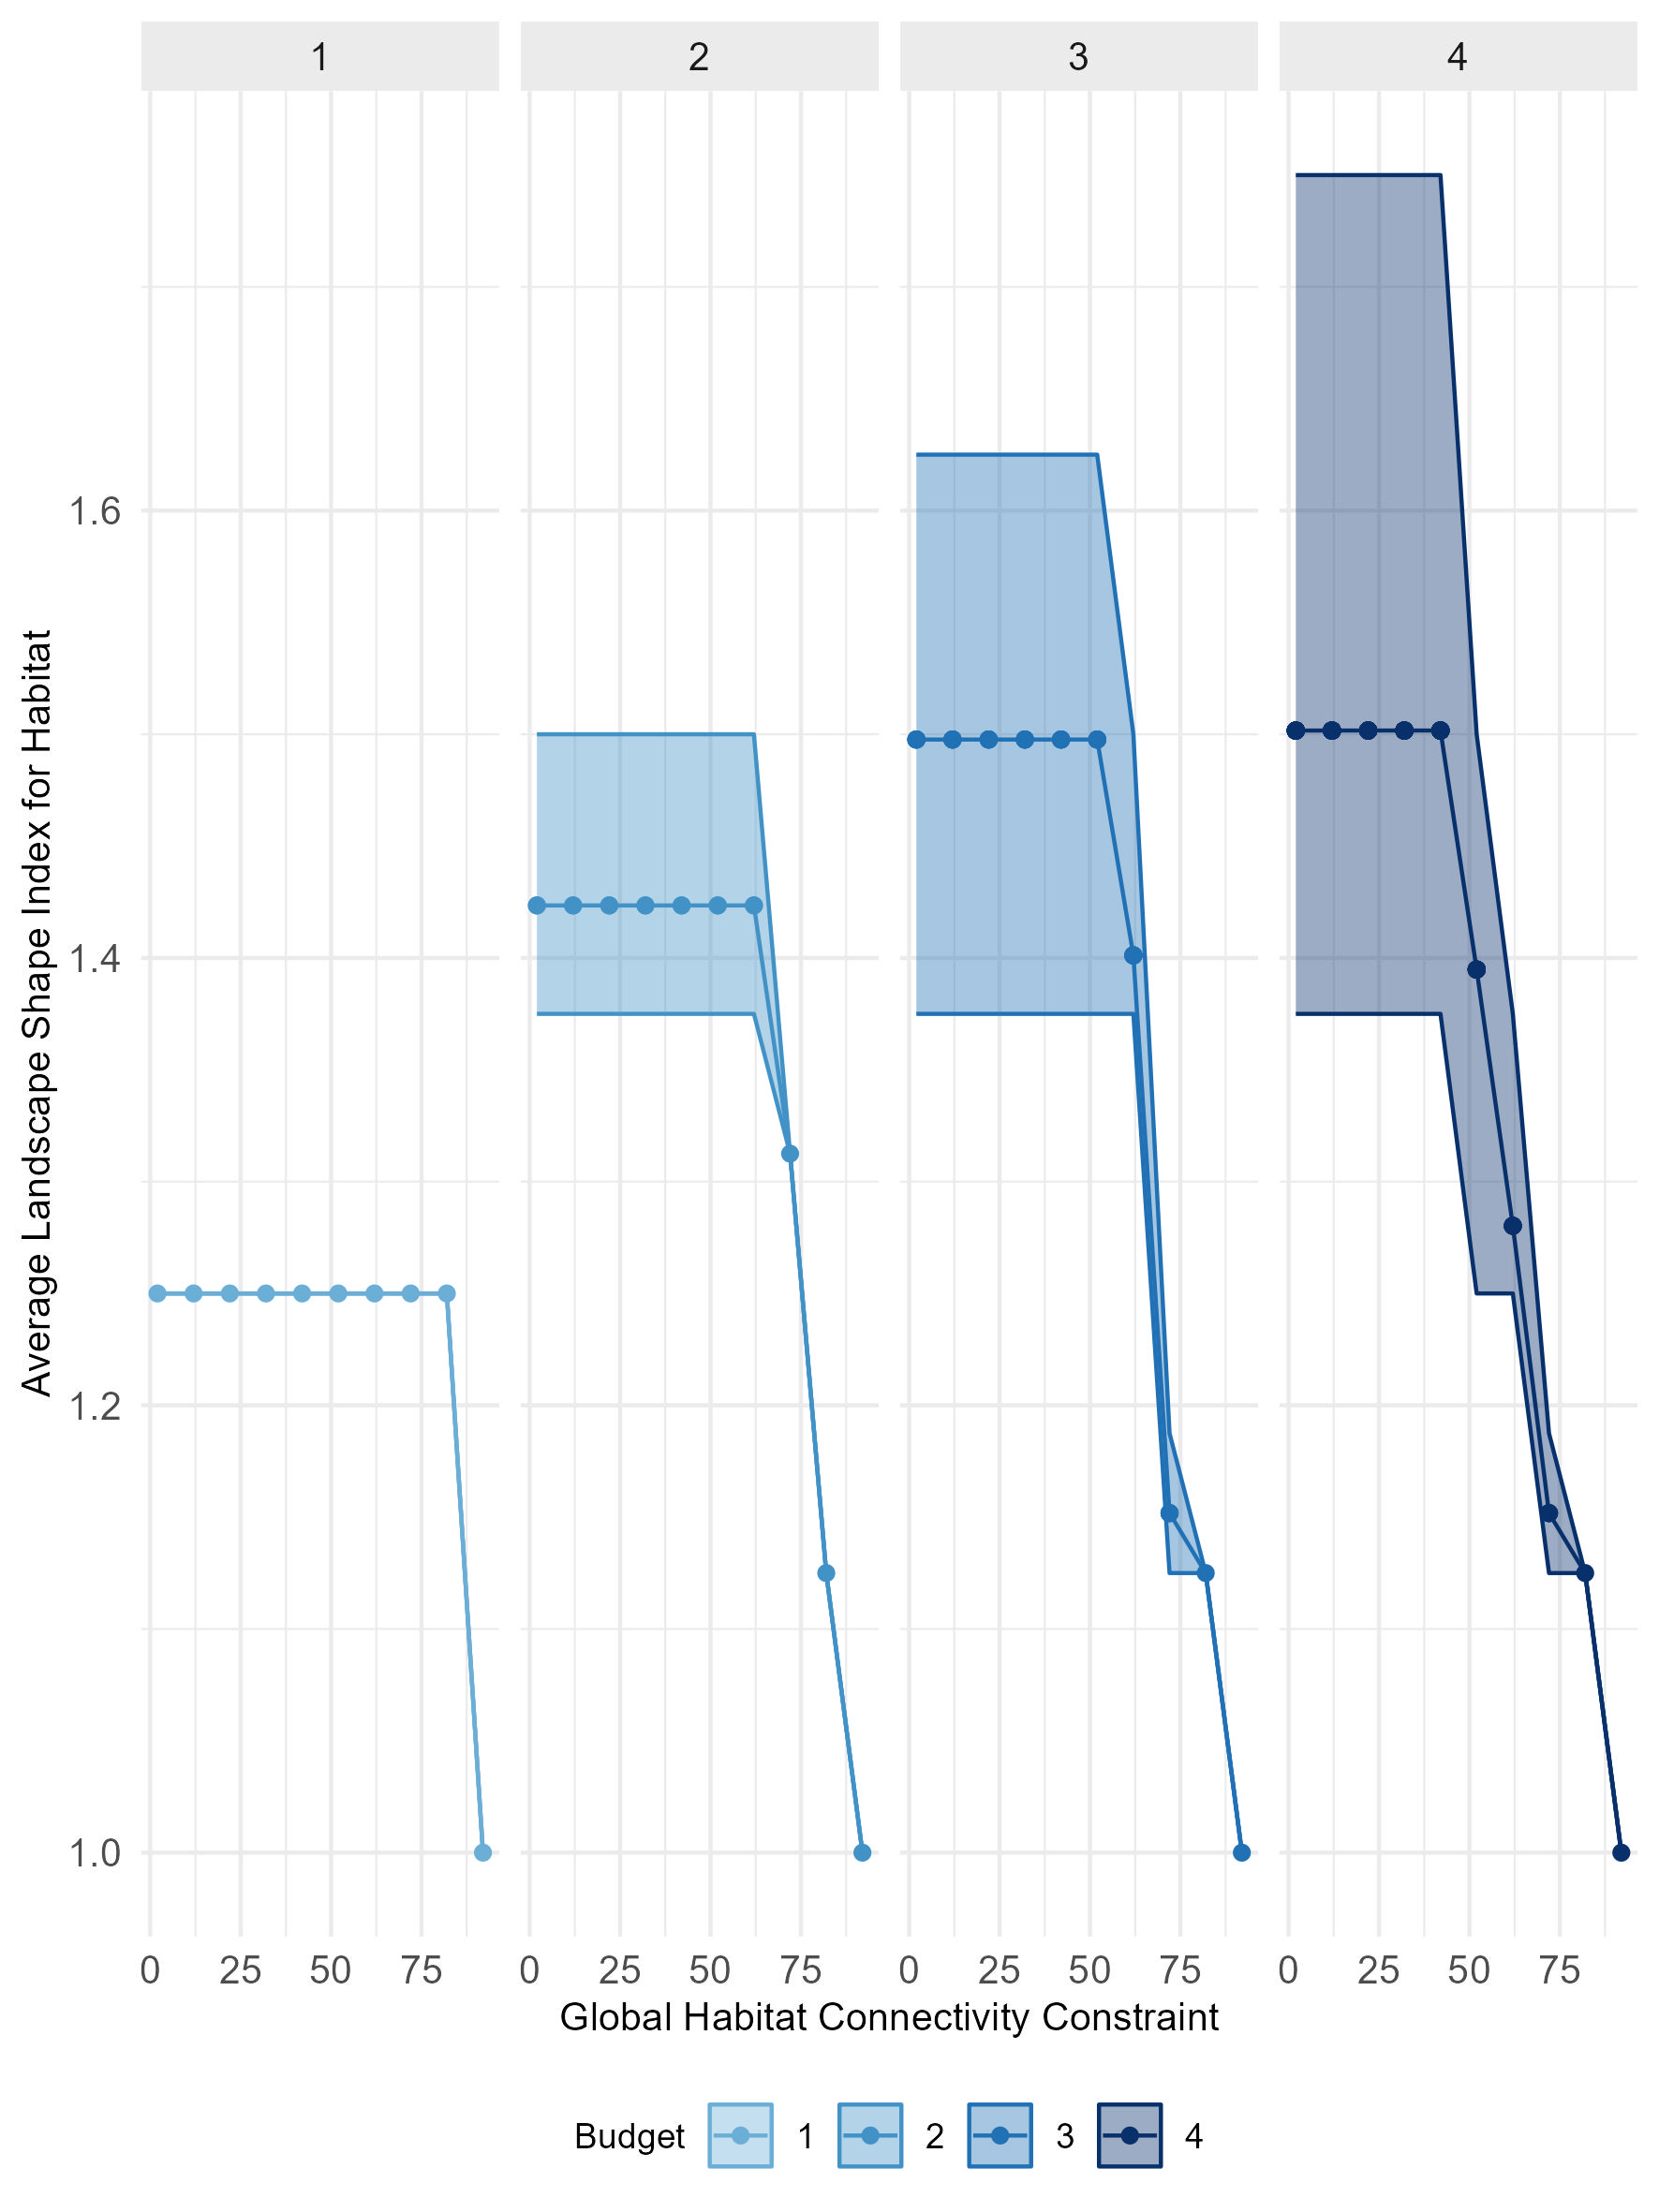
\includegraphics[height = .3\textheight]{figures/wildland/average_LSI_B.jpg}
        \caption{Average Landscape Shape Index for Habitat}
        \label{fig:lsi}
    \end{subfigure}
    
    \caption{Indicators relative to landscape diversity across habitat and budget constraints}
    \caption*{The indicators are averaged across the cycles represented for each habitat and budget constraint levels.}
    \label{fig:indicators2}
\end{figure}


Previous results show that budget further reduces risk, conditional on habitat connectivity constraint being low. Focusing on constraint levels below $50$,  risk reduction is primarily driven by reduced area (figure \ref{fig:area}), and increased fragmentation of the landscape, in the form of increased components number and reduced sized of the components mean size (figures \ref{fig:component_number} and \ref{fig:components_size}). As more connected habitat needs to be protected, the average size of components increases for all $Budget>1$. For large budgets (e.g. $Budget \in\{3,4\}$), the average component number starts to fall first (for example, at habitat connectivity constraint level $40$ for $Budget = 4$), and then the average risk area increases (for example, at habitat connectivity constraint level $52$ for $Budget=4$). The average component size increases as the number of components decreases for habitat connectivity constraints above $42$ : small components either disappear or increase in size, risky cells are reallocated to connect separated components before the high-risk surface increases. 
 This is exemplified by the landscape cycles displayed in figure \ref{fig:cycles} (especialy for panels of $Budget \in \{3,4\}$).


Landscape diversity unambiguously increases with the budget at low habitat connectivity constraint levels (figures \ref{fig:simpson} and \ref{fig:het}). As more units are treated, the evenness of successional stages increases in the landscapes, which drives increases in the Simpson Index (fig. \ref{fig:simpson}). At low habitat connectivity constraints, global risk connectivity is diminished through fragmentation of the risky patches. The larger the budget, the more treatment, and the more fragmentation, which increases the structural diversity of the landscapes as cells are less likely to be at the same successional stage in all directions, driving the evolution of the Successional Stage Hetergoeneity Index (fig. \ref{fig:het}).
At low habitat connectivity constraint levels and large budgets, even though the relative area of habitat decreases, the shape of habitat is more irregular (fig. \ref{fig:lsi}). In this context, \textit{adolescent} cells act as stepping stones and corridors between \textit{mature} habitat patches. 

When habitat connectivity constraints increase, diversity collapses both quantitatively and qualitatively (fig. \ref{fig:indicators2}). The Simpson index collapses as land successional stages gradually homogenize (fig.  \ref{fig:simpson}) across all budgets. Moreover, landscapes form less of a mosaic, and are more clumpy, as displayed by the LSI and Successional Stage Heterogeneity Index (figs. \ref{fig:lsi} and \ref{fig:het}). Overall, for large habitat targets, landscapes tend to homogenize and to be better connected, although less quantitatively and qualitatively diverse. 
%\begin{enumerate}
%    \item Budget
%    \begin{itemize}
%        \item When budget is large, we have seen that risk is low(er). How?
%        \item The overall area is lower when budget is large  : more cells are being treated. 
%        \item Moreover, the number of disconnected subgraphs tends to increase, as the budget increases : the wildfire risk is fragmented and spread on the landscape (unless the budget is large enough that only 1 small component remains in the landscape for case 3)
%        \item Moreover, the size of at risk components decreases with budget. 
%        \item \textbf{Need to find the angle for diversity} : diversity increases with budget, as more patches can be treated (simpson and shanon). From a spatial perspective, for a lax requirement, it also increases diversity, where diverse patch are well connected to the rest of the lansdcape. It is a well connected diversity because the LSI is large. 
%    \end{itemize}
%    \item Habitat constraint 
%    \begin{itemize}
%        \item As biodiversity connectivity requirements increase, the risky area increases, and the number of components tends to decrease : more habitat patches need to be connected. 
%        \item Interestingly, there is a trade-off between : adding 1 patch (vertex) to a component such that it is not connected with the rest of the graph, or not adding one, but such that it connects components. 
%        \item \textbf{Framing here} : diversity tends to decrease with biodiversity requirement, both quantitatively and qualitatively
%        \begin{enumerate}
%            \item Find story for the lower budget above the larger for LSI : more area in lower budget, so maybe that's overall better. 
%            \item Fit a discussion point : our metric focuses on a single species, and we show that id functional diversity needs to be accounted for, then single species habitat is not the right metric
%        \end{enumerate}
%    \end{itemize}

%\end{enumerate}

\FloatBarrier
\subsection{Spatial allocation of optimal management at the steady-state landscape cycle}

Treatments are concentrated on \textit{adolescent} cells across all budget and habitat connectivity constraints (figure \ref{fig:treatments_time}, except at $62$, for some steady-state cycles for $Budget \in \{3,4\}$). This is coherent with the real life practice of fuel management operations, primarily targeting \textit{adolescent} land patches. At level $62$, the number of treatment varies between phases of the steady-state cycle for $Budget=4$, reflecting the increase in habitat connectivity constraint. 

\begin{figure}
         \centering
         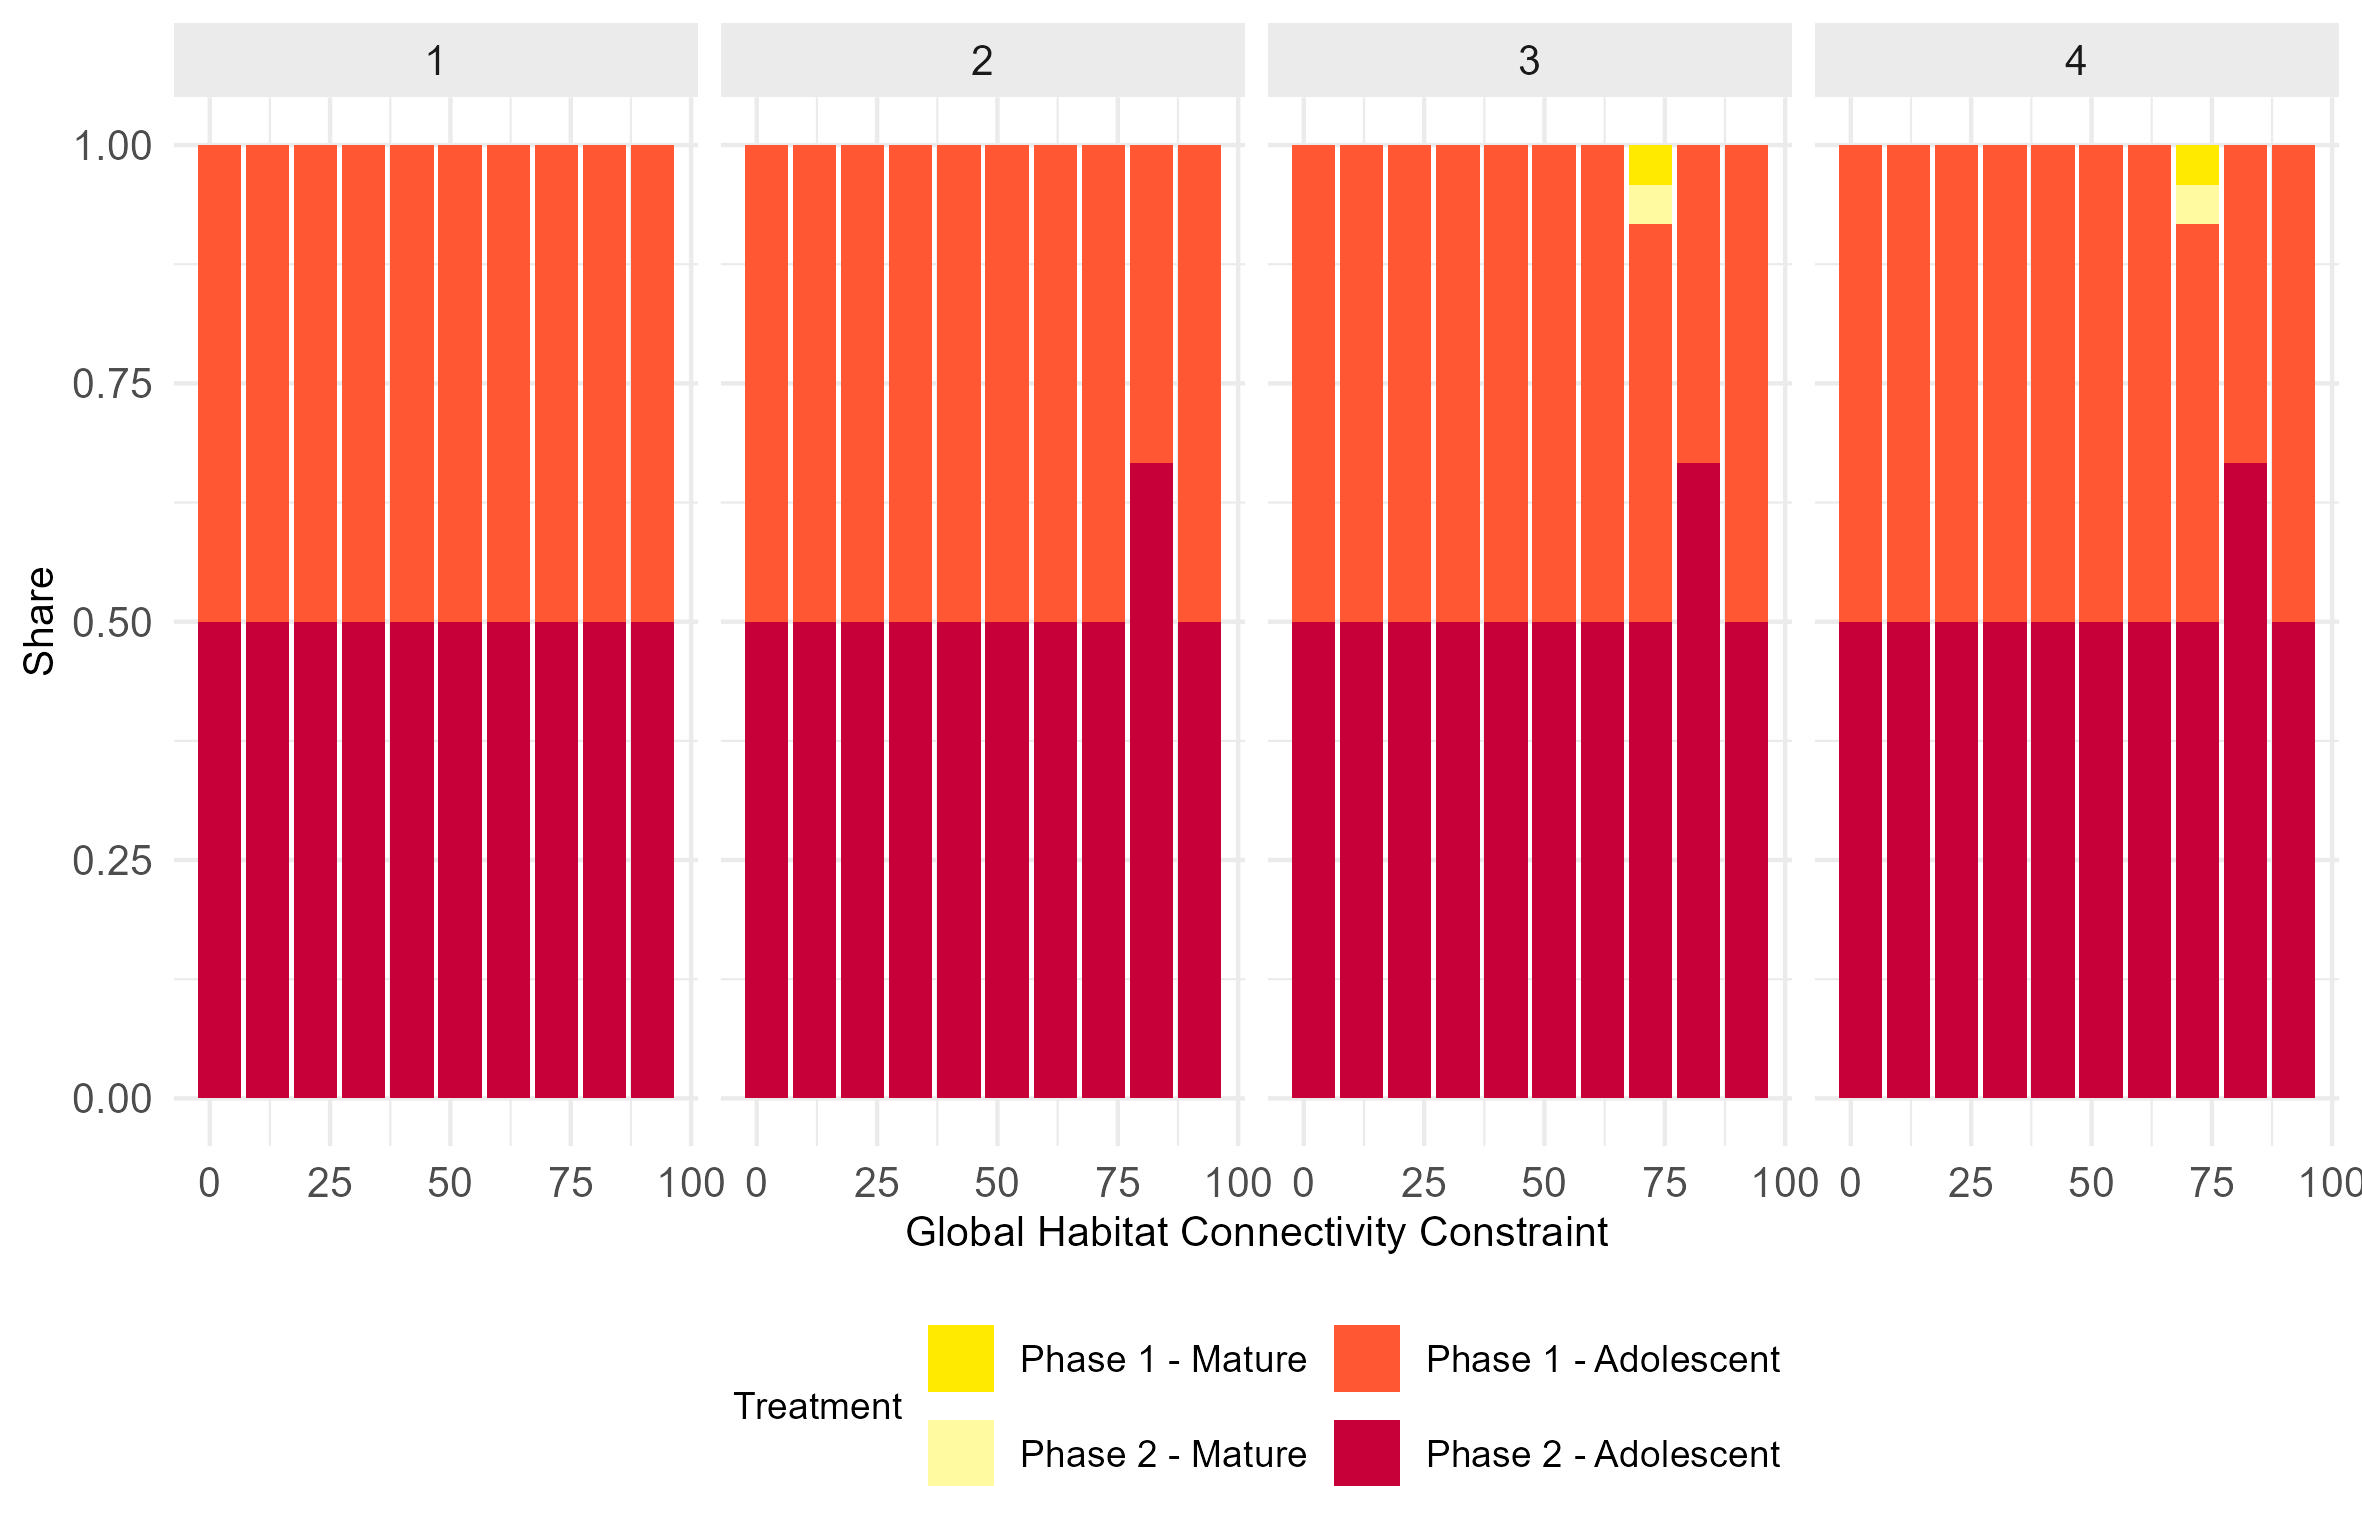
\includegraphics[width=.8\textwidth]{figures/wildland/treatment_time.jpg}
    		  \caption{Distribution of the successional stages of treated cells in steady state cycles across budget and habitat connectivity constraints}
         \label{fig:treatments_time}
\end{figure}

As show in figure \ref{fig:treatments_number} for low habitat connectivity constraints, the budget constraint is saturated, and all of the budget is used. Coherent with the evolution of risk area highlighted in section \ref{sec:landscape_char}, the number of treatments decreases after the steady state landscape start experiencing an increase in mean component size, and gradually reduce as the habitat connectivity constraint increases (e.g. starting at $62$ for $Budget = 2$, or $52$ for $Budget = 4$): for large habitat connectivity constraints, the budget constraint is no longer satiated. 
 
\begin{figure}
     \centering
         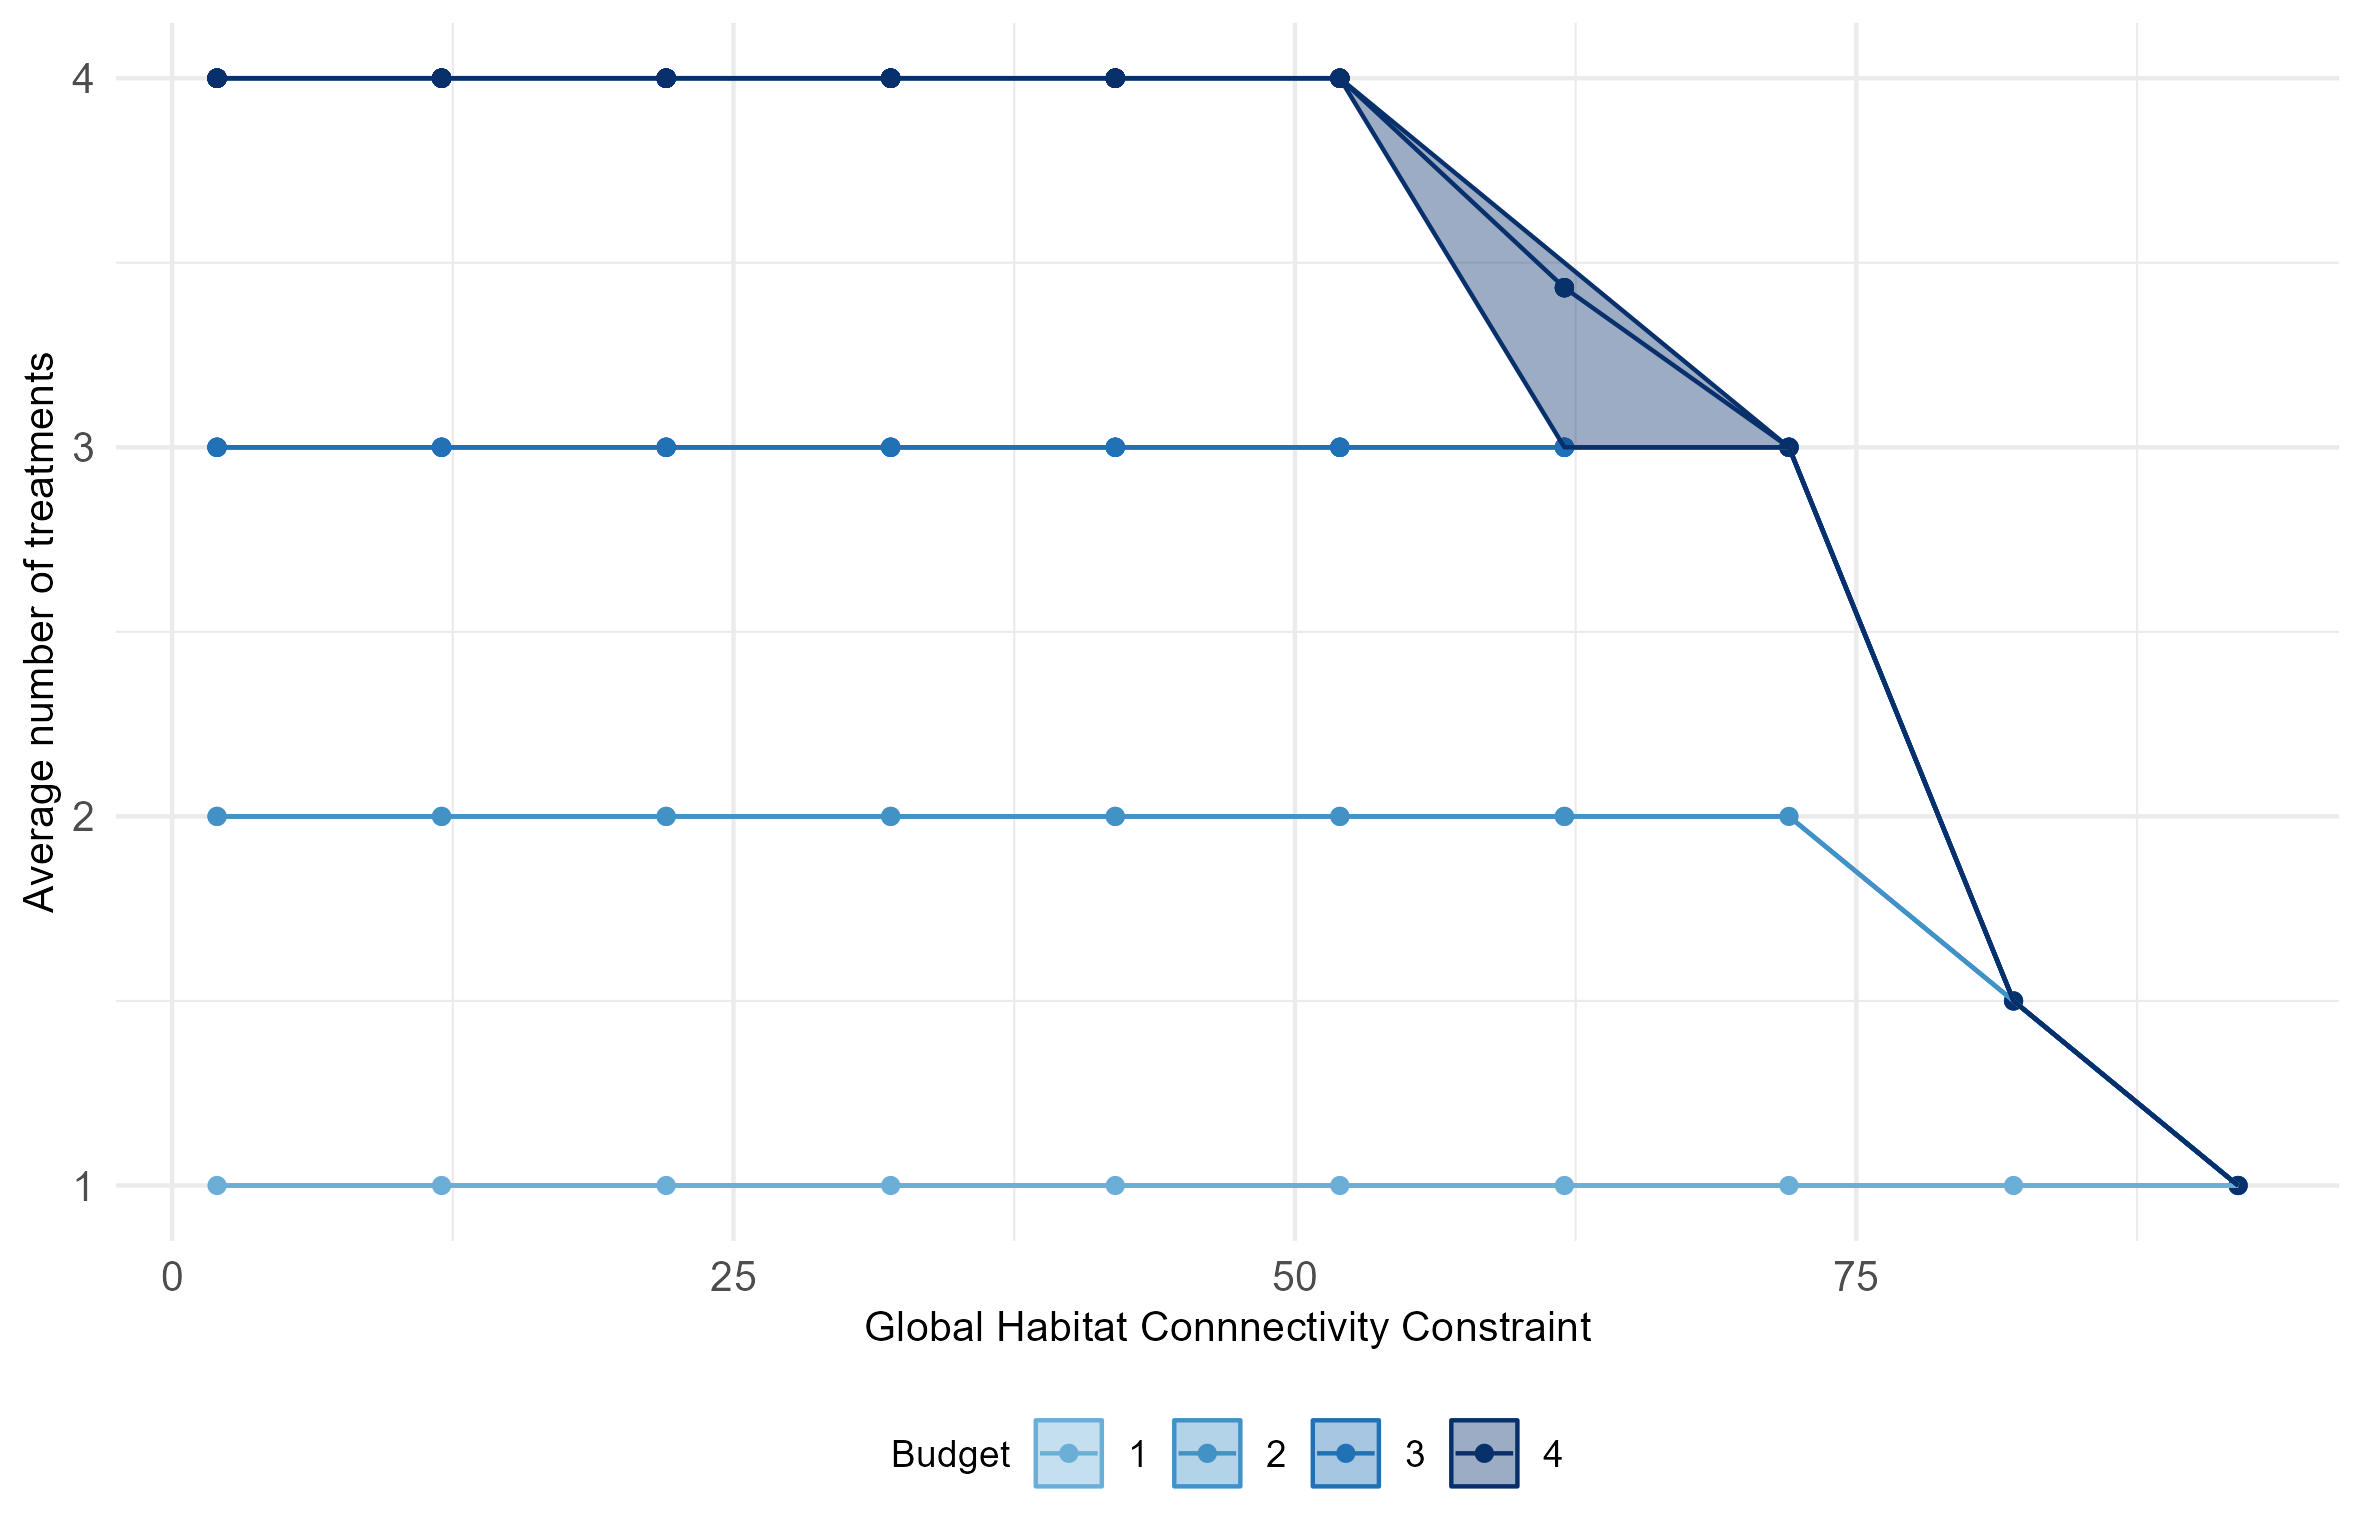
\includegraphics[width=.8\textwidth]{figures/wildland/number_treatments.jpg}
         \caption{Average number of treatments in steady state cycles across budget and habitat constraints.}
         \label{fig:treatments_number}
\end{figure}

Figures \ref{fig:between}, \ref{fig:subgraph}, \ref{fig:degree} and \ref{fig:eigen} show that the different centrality measures (e.g. betweenness, subgraph, degree and eigencentrality, respectively), are very correlated, and display identical overall patterns, in terms of relative values of metrics compared to the maximum possible, and in terms of rankings. We therefore focus on betweenness centrality to characterize our results. 

Figure \ref{fig:between} shows the average betweenness centrality (and the corresponding ranking) of treated cells in risk graphs $\mathcal{F}_t$. For low levels of biodiversity constraint, cells with the largest betweenness centrality are treated first, as testified by the panel of $Budget=1$ in figure \ref{fig:between}, and illustrated by the average share of treatments per cell in figure \ref{fig:treatments_location}. Across budgets, the first treatment unit targets the most central cells when available for treatment. In the context of critical node detection, when the ecological requirements are low, the high-risk graph $\mathcal{F}_t$ is primarily considered, and nodes with the most cost-efficient risk reduction, i.e, with the largest betweenness centrality are targeted. Once the most connected cells are treated and the budget constraint relaxes, lower-centrality cells get treated, in a sequential fashion. : for $Budget=4$ and constraint below $42$, the first treatments across cycles are the $1^{\mathrm{st}}$ and $2^{\mathrm{nd}}$ most central locations, but the $4^{\mathrm{th}}$ treatments target the least central cells with non zero centrality. This is epitomized by the top row of figure \ref{fig:treatments_location}.  

\begin{figure}
     \centering
     \begin{subfigure}[b]{\textwidth}
         \centering
         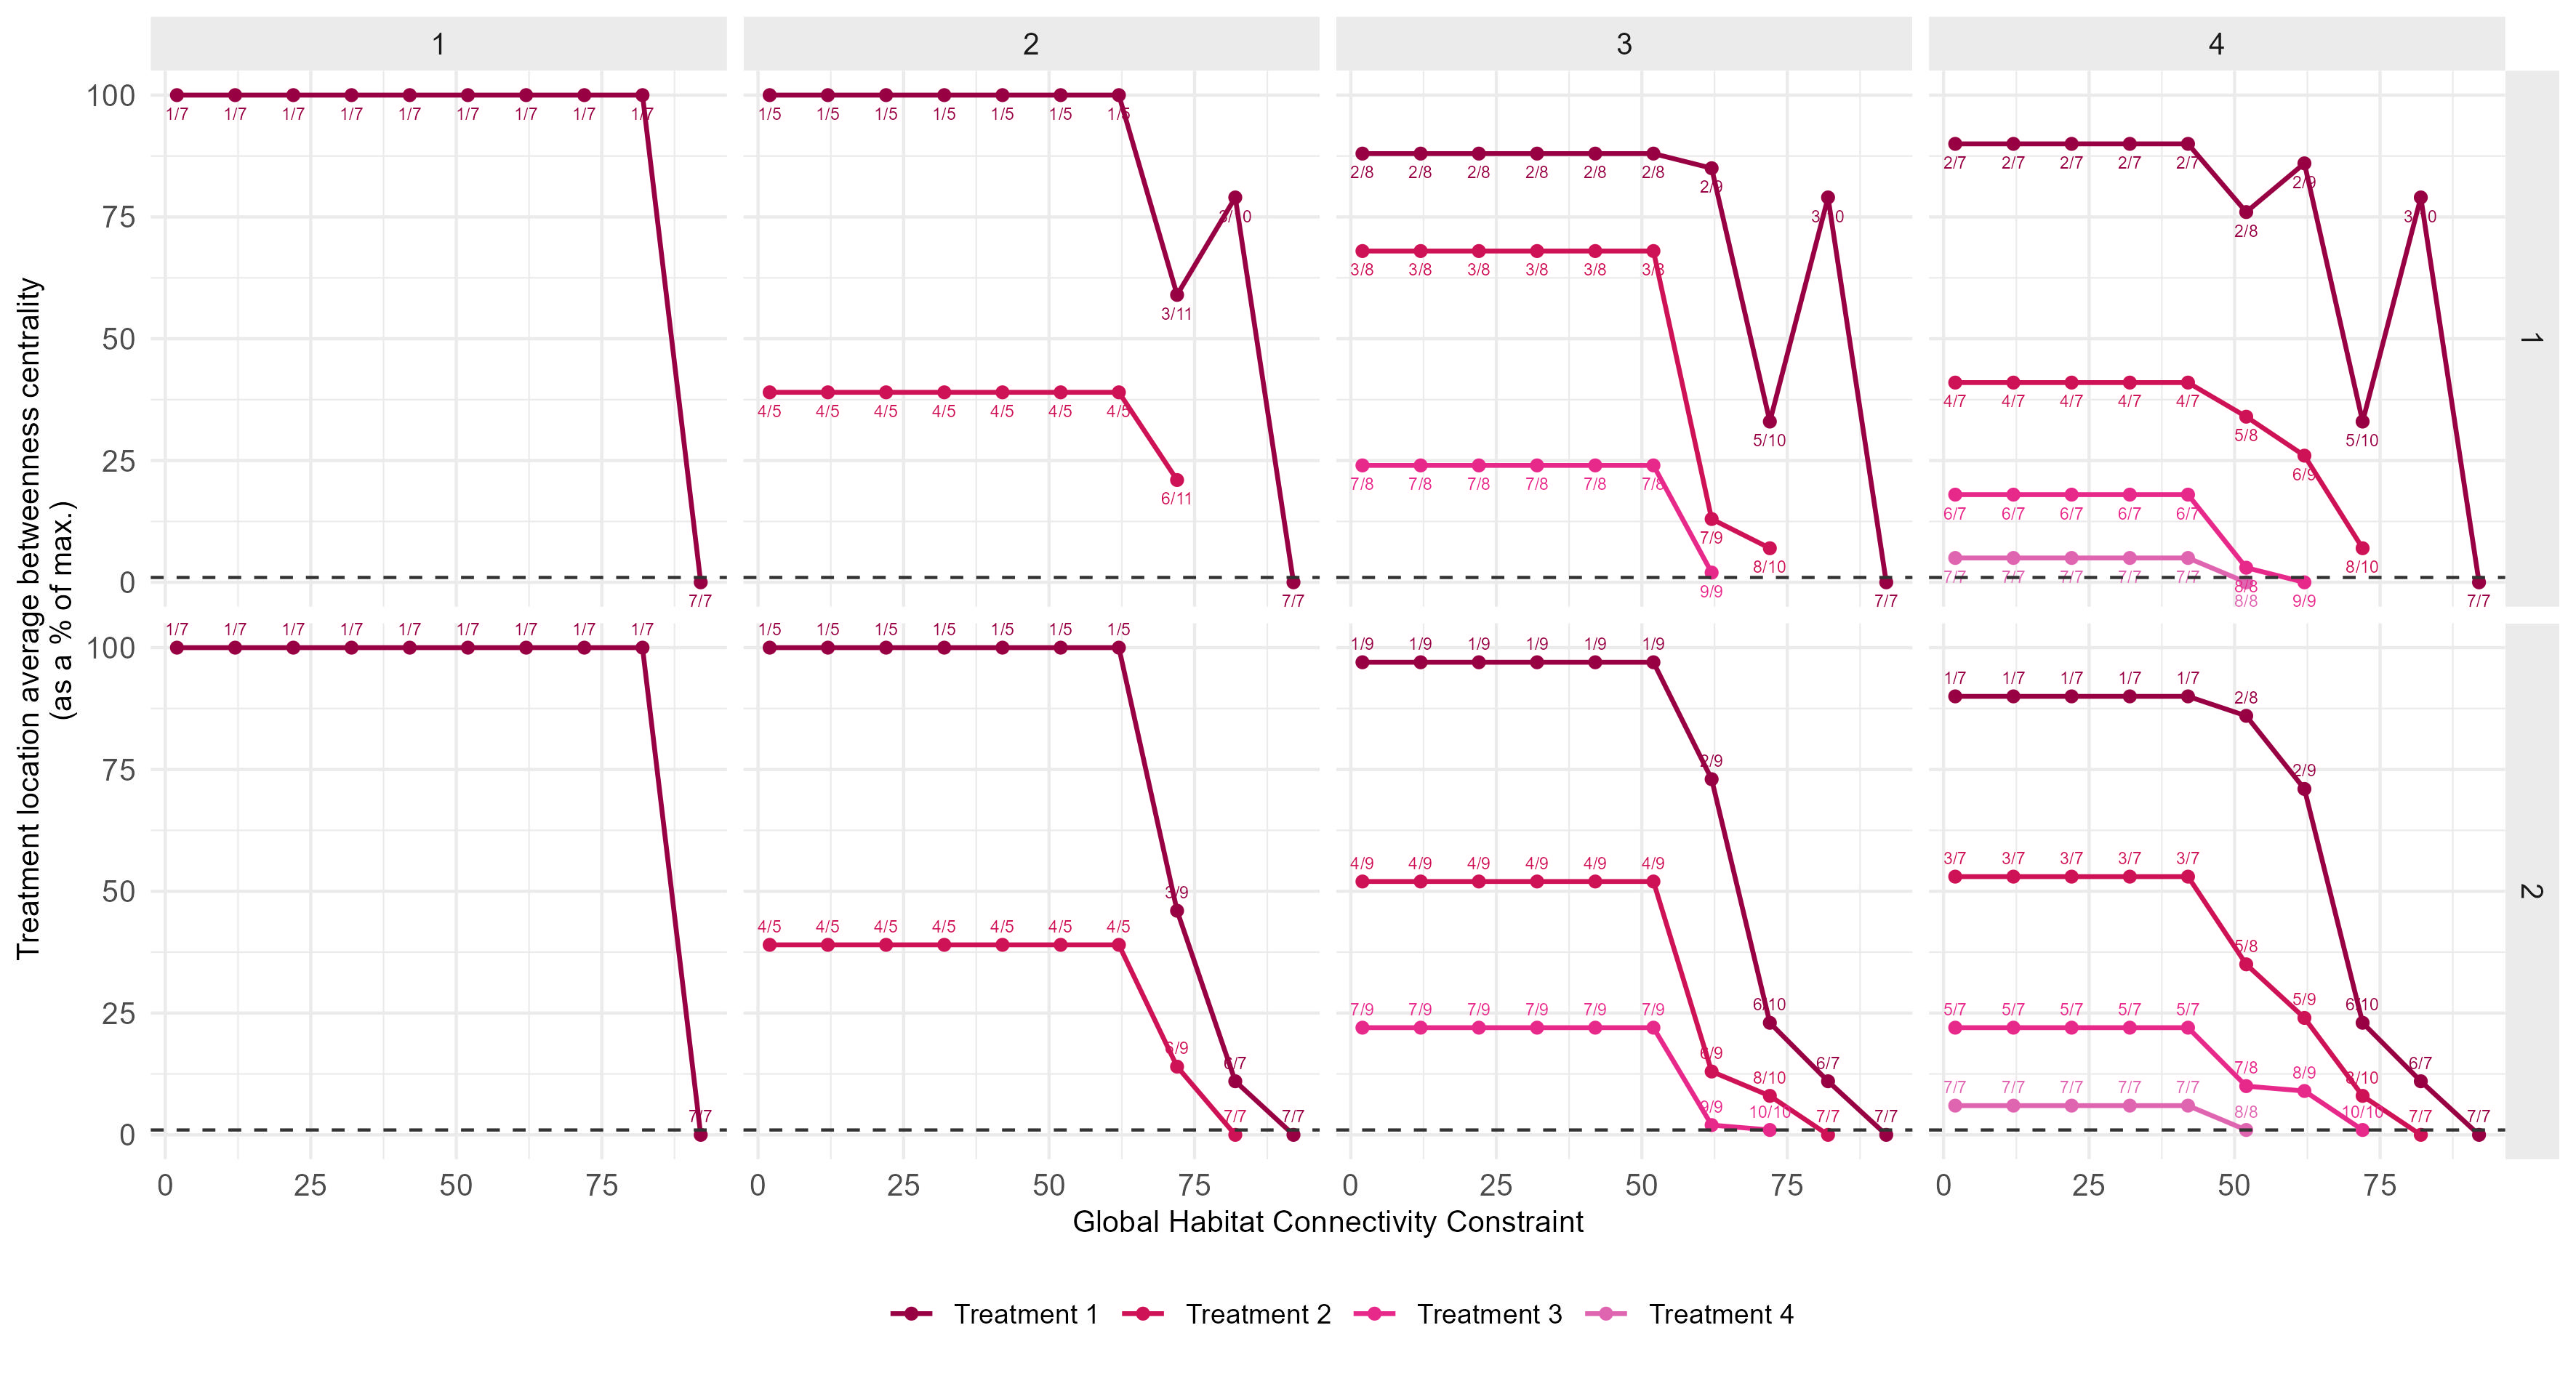
\includegraphics[width=\textwidth]{figures/wildland/betweenness_treatment.jpg}
         \caption{Average treatment location betweenness centrality across budget and habitat connectivity constraints, and steady-state cycle phases}
         \caption*{On the horizontal grid are displayed budget levels, while cycle phases are displayed on the vertical grid. For each steady-state cycle, treatment location is characterized by a betweenness centrality score, as a proportion of the maximal betweenness. Averages across steady-state cycles are displayed. Numbers in $5/7$ format refer to the average betweenness centrality ranking of the treatment} 
         \label{fig:between}
     \end{subfigure}
     \begin{subfigure}[b]{\textwidth}
              \centering
		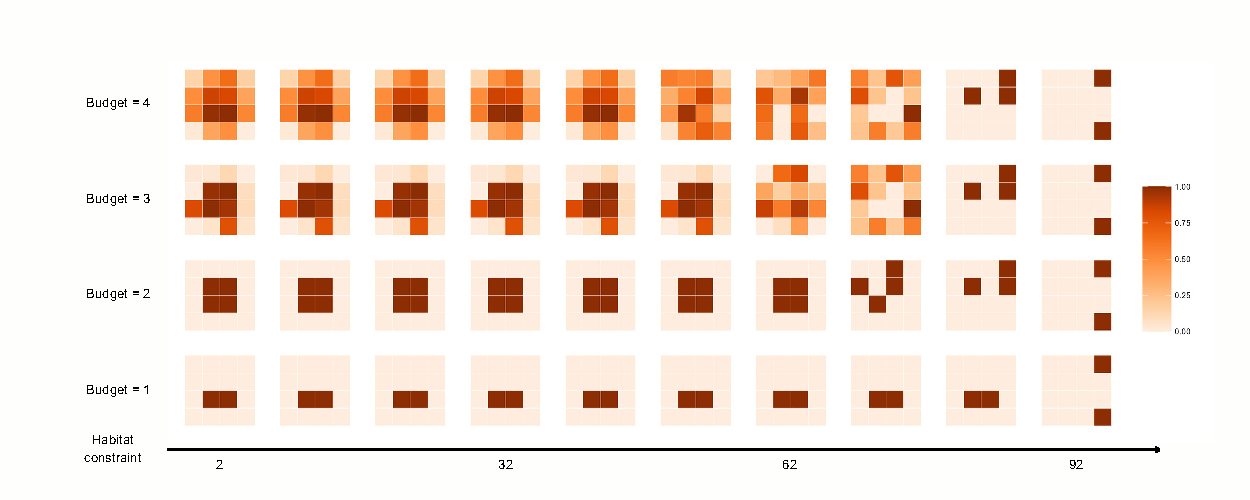
\includegraphics[width=\textwidth]{figures/wildland/average_treatments_legend.pdf}
    		  \caption{Distribution of treatment locations in steady-state cycles across budget and habitat connectivity constraint levels}
    		  \caption*{Each cell is colored as the average of her treatment indicator $x_{ijt}$ over all steady-state : the darker the cell, the higher the frequency of treatment}
     \label{fig:treatments_location}
     \end{subfigure}
     \caption{Treatment allocation : centrality}
     \label{fig:centrality}
\end{figure}

When the habitat connectivity constraint increases, several effects come at play. Not only does the number of treatments decrease, but the spatial allocation also changes. When $Budget=3$, figure \ref{fig:treatments_number} shows that treatment number remains constant between habitat connectivity constraints $52$ and $62$, but the spatial distribution of treatments drastically changes (fig \ref{fig:treatments_location}), as treated cells are less central, and edge cells are more treated (fig \ref{fig:between}) as the relative weight of the habitat graph $\mathcal{B}_t$ increases, treating the most cost-efficient risk-reducing nodes also degrades habitat connectivity.

Therefore, as habitat targets increase, the number of treated cells remains stable but the betweenness centrality of cells decreases : for $Budget=2$, aggregate betweenness centrality starts declining at $62$, for $Budget=4$ at $42$ (figs \ref{fig:centrality} and \ref{fig:treatments_location}). Then, the number of treated cells decreases : for $Budget=2$ for example, treated cells start declining at $82$, and for $Budget=4$ at $52$ (fig \ref{fig:treatments_number}). Once the number of treated cells has decreased, there is a spike in betweenness centrality of the remaining treated cells : while less area is treated, a more central location is treated (see the panel of phase 1 and $Budget \in \{2,3,4\}$ at levels $82$). Then, the number of treated cells continues to decrease as the habitat connectivity constraint increases, and less central cells are targeted. 

Considering results in terms of pattern convergence and treatments charactistics, general treatment guidelines can be derived and applied to large scale landscape, with a budget comprised between 0 and 25\% of the landscape size. As measures of connectivity can be correlated at the small scale, but differ at the large scale, we formulate 4 different strategies, where centrality is defined according to the 4 measures used : 
\begin{enumerate}
\item For low habitat requirement (e.g. below 50\% of maximal global habitat connectivity), the budget constraint must be saturated and target cells with the largest betweenness centrality. For the first 5 periods, target cells can be both \textit{adolescent} and \textit{mature}

\item For intermediary habitat requirements (between 50\% and 75\% of maximal global habitat connectivity), and low budget, the budget constraint must still be saturated, but for larger budgets, decreased by 25\%. 25\% of the budget can be spent on high betwennness centrality cells, but 75\% of the budget must be spent on average or low betweenness centrality cells

\item For large habitat requirements (between 75\% and 100\%), the budget constraint must not be saturated:  the percentage of treated cells must decrease to an interval between 5 and 15\%, and low betweenness centrality must be targeted if any cell is to be treated. 
\end{enumerate}
Across all these options, to account for the transitionary dynamic, target cells can be both \textit{adolescent} and \textit{mature} in the first 5 periods, and exclusively \textit{adolescent} for the last 5. We use these principles to structure treatment rules for large scale landscapes, and compare them to optimal management as well as other policy rules. 

%\renewcommand{\arraystretch}{2}
%\begin{table}[h]
%   \centering
%   \resizebox{.7\textwidth}{!}{
%    \begin{tabular}{|c|c|c|c|}
%    \hline \hline
%         & \textbf{Habitat target} & \textbf{Low} & \textbf{Large} \\
%    \hline
%     \textbf{Budget}    &  \textit{Number of treatments} & \multicolumn{2}{c|}{\textit{Decreasing}}\\
%    \hline
%   \textbf{Low} & \multirow{3}{*}{\textit{Increasing}} & Most central nodes   & Edges and corners\\
%   \cline{3-4} \cline{1-1}  
%     \textbf{Large} & & Most central nodes  & Less central nodes,\\ 
%      & & and lower degree nodes &  edges and corners\\
%     \hline \hline
%    \end{tabular}}
%    \caption{Spatial treatment allocation in landscapes $n=3,4$}
%    \label{tab:synth_treatments}
%\end{table}

\FloatBarrier

\subsection{Evaluating policy rules }
\label{sec:evaluating_policy}
Figure \ref{fig:comparison_policies} and \ref{fig:comparison_constraints} shows the performance of the diverse policy options across 20 large scale landscapes on planning horizon of $10$ periods. The performance is assessed as the sum of the global risk connectivity across 10 periods and a penalty proportional to the difference between the global habitat connectivity constraint and the global habitat connectivity score across periods. 

\begin{figure}
\centering
    \begin{subfigure}[b]{.8\textwidth}
	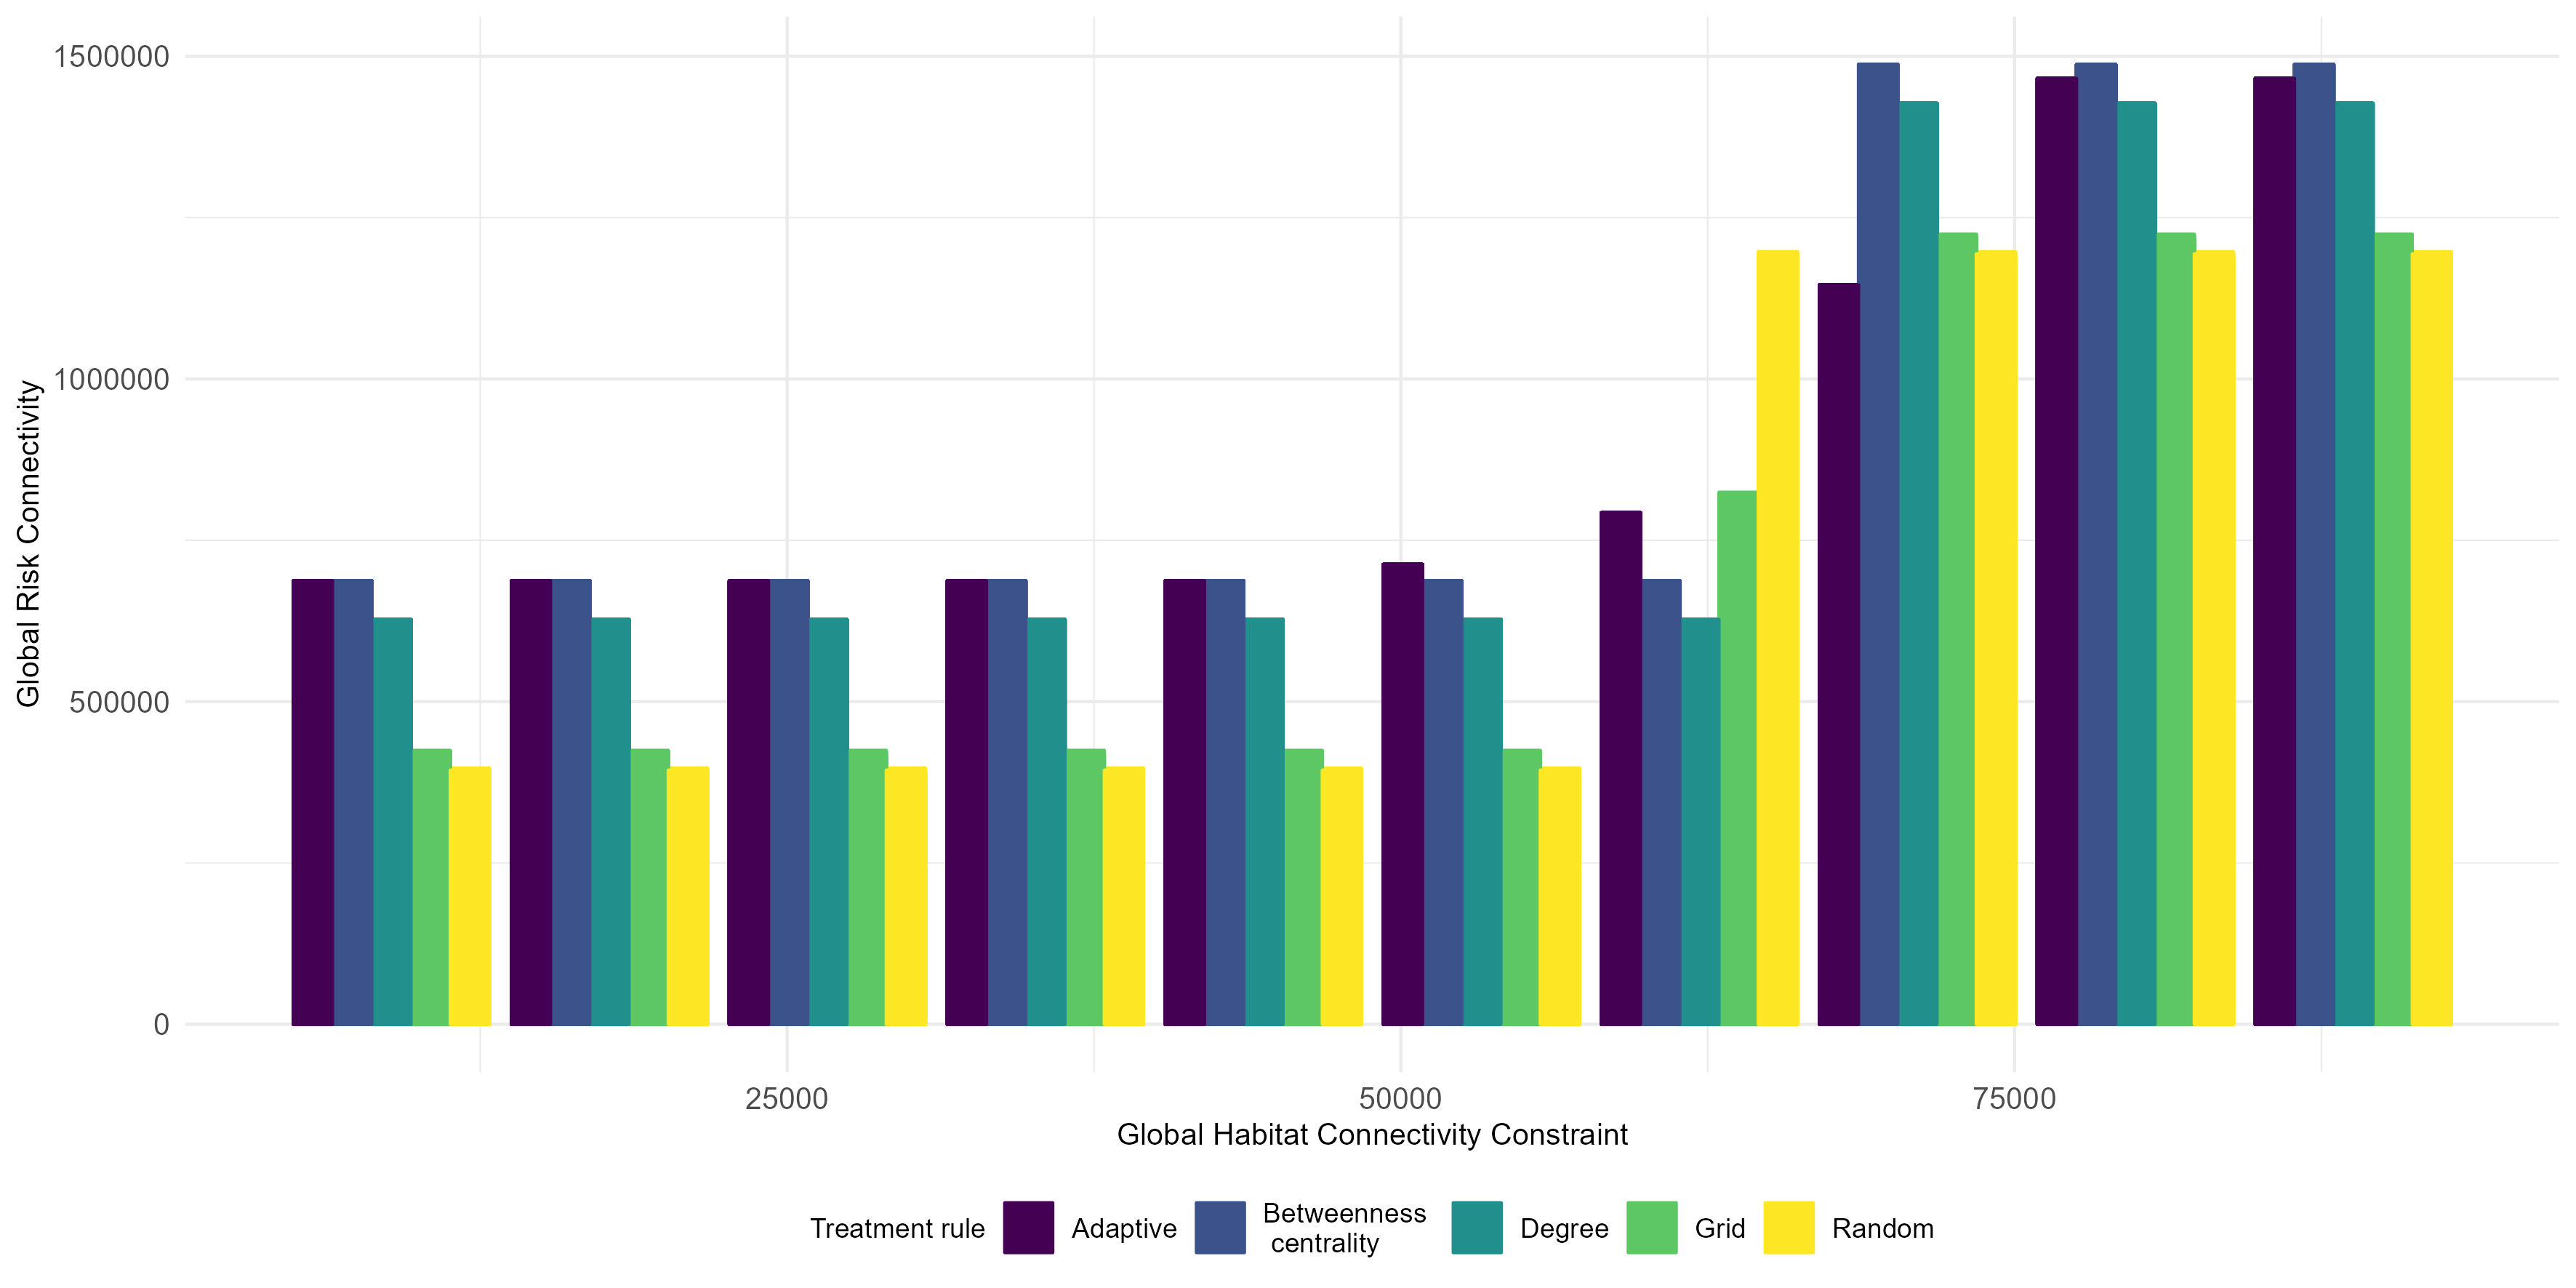
\includegraphics[width=\textwidth]{figures/wildland/comparing_performances.jpg}
\caption{Comparison of policy intertemporal risk and penalty for large scale landscapes}
	\label{fig:comparison_policies}
	\end{subfigure}
	\begin{subfigure}[b]{.8\textwidth}
	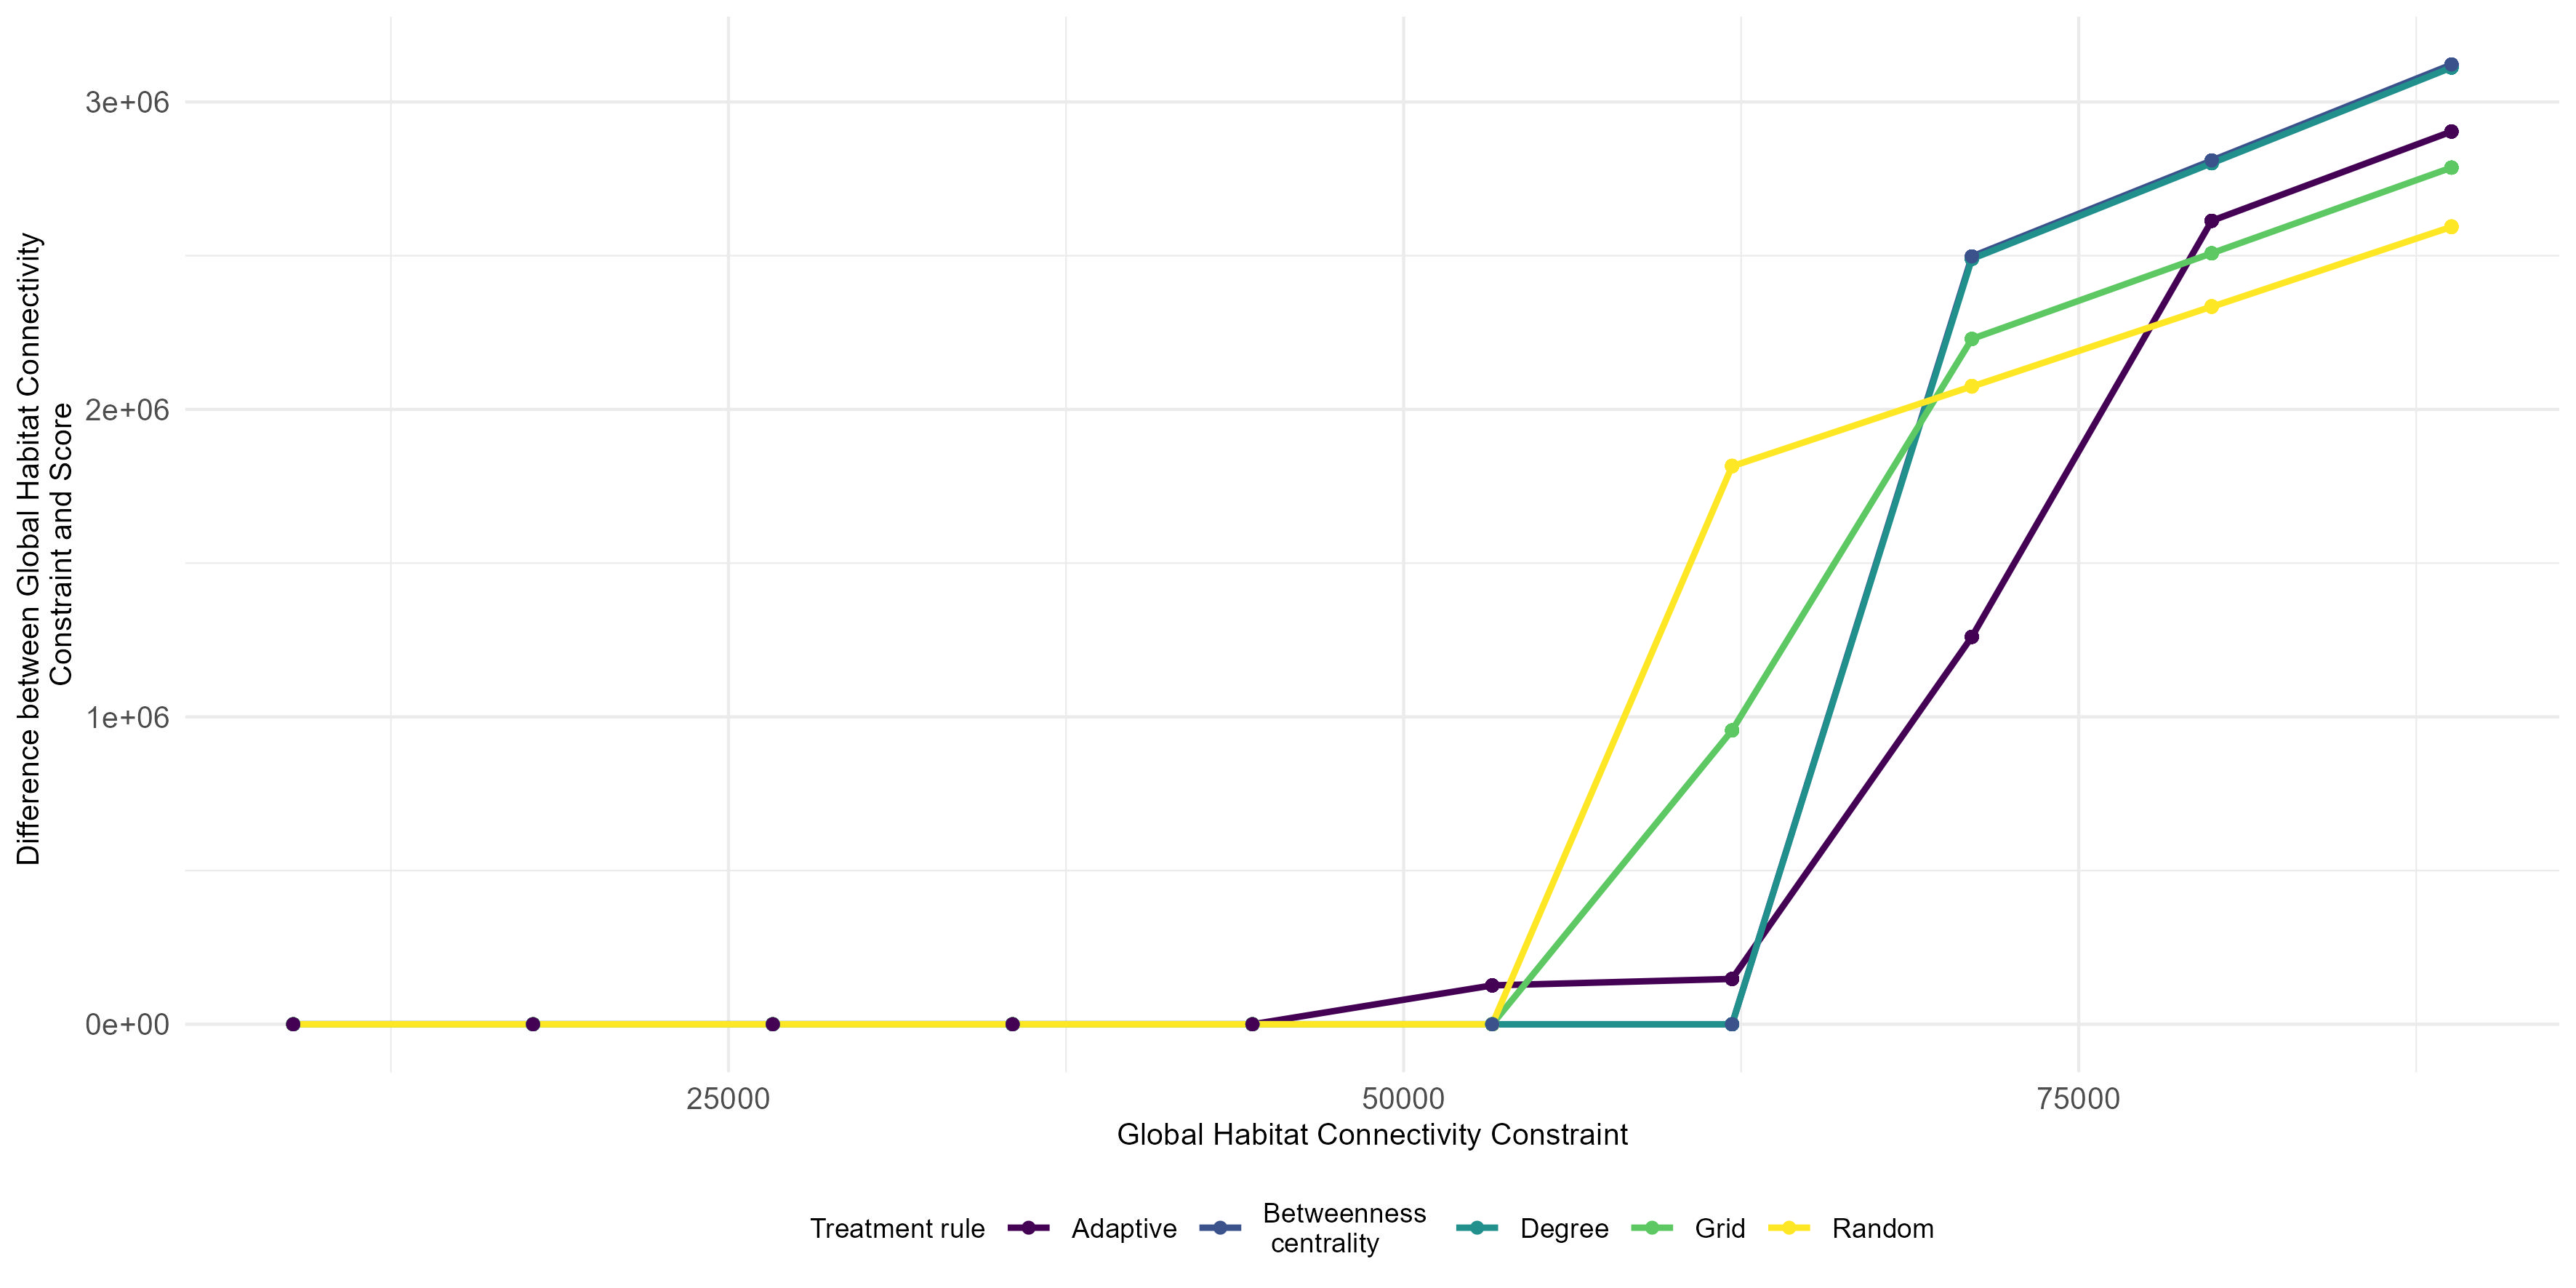
\includegraphics[width=\textwidth]{figures/wildland/comparing_performances_biod.jpg}
\caption{Comparison of global habitat connectivity constraint attainments for large scale landscapes}
	 \label{fig:comparison_constraints}
	 \end{subfigure}
	 \caption{Comparison of policy performances for large scale landscapes}
\end{figure}

Results show that the grid and random policy rules  fare better than the policies based on graph theory metrics for constraint values below $61,262$ (e.g. 70\% of maximal global habitat connectivity). At $61,262$, they fare worse than the metrics based on graph theoretical measures, but the adaptive strategy extrapolated from small scale results fares worst among graph theory policies. At $71,403$ (e.g. 80\% of maximal global habitat connectivity), the adaptive strategy fares better than all measures, as only it is the only one that satisfies the habitat connectivity constraint. After $71,403$, the adaptive strategy is ranked 3rd after the random and grid strategies, as the difference in global habitat connectivity constraint attainment rises faster than with the random and grid policies.

\section{Discussion}
\label{section:discussion}

\subsection{Confirmation and generalization of existing results}
Our analysis of the exhaustive set of initial conditions for small-scale landscapes confirms existing results in the literature. We argue that they bring robust evidence and complement the existing literature to derive general conclusions. 

Our model encompasses 3 seral stages and 1 composite vegetation type and proves the convergence of every initial condition to a steady state cycle, irrespective of the initial configuration. We extend \cite{minas_spatial_2014} that find convergence patterns for \textit{homogeneous} landscapes only, i.e, landscapes where the initial vegetation age is uniformly distributed.  We show that in the event of environmental perturbations that do not disrupt ecosystem dynamics, an appropriate policy can recover the previous equilibrium risk and habitat. 
%Additionally, small scale results efficiently guide rules for larger landscapes : patterns can indeed be identified using a graph-theoretical framework. 
%We hypothesize that as long as the risk/ successional-stage relationship reaches a plateau for every vegetation type on the landscape, convergence should be observed.

Our production possibility frontier (PPF) between wildfire risk and habitat connectivity is consistent with PFF literature \citep{arthaud_methodology_1996,calkin_modeling_2005}. Our results also confirm that trading one objective for the other is not as efficient as increasing the policy budget to reconcile objectives. We show that increasing the policy budget nonetheless has diminishing returns for risk reduction, as highlighted by \cite{wei_optimization_2008, yemshanov_detecting_2021} and \cite{pais_cell2fire_2021}. 

Our study yields clear results in terms of landscape ecology, leveraging concepts from landscape ecology, and highlighting the spatial mechanisms underlying the shape of PPF. We show that, for small scale, treatment allocation targets the most (between) central nodes first and then focuses on less central nodes (e.g cells closer to the border of the landscape) when habitat goals are low. In doing so, we do find general treatment allocation principles where previous studies on larger landscapes could not \citep{minas_spatial_2014, rachmawati_optimisation_2016}, generalize smaller scale \citep{konoshima_spatial-endogenous_2008} and case study specific \citep{yemshanov_detecting_2021, pais_downstream_2021} results.

Compared to existing studies, our bounded depiction of vegetation dynamics allows, as well as the timing of decision making makes repeated myopic and dynamic approaches almost identical. As we abandon the refinement of dynamics, we are able to analyze the whole range of initial conditions, an endeavor that is seldom possible in dynamic spatial modeling. Using a graph theoretic framework on small-scale landscapes, we show that cell-level metrics help formalize and understand the drivers of treatment allocation and rationalize existing results. 

Furthermore, we show that while prioritization approaches based on a graph theoretic framing fare very well in an unrestricted set-up, including biodiversity habitat targets augments the problem's complexity. As a matter of fact, critical node detection can be efficiently achieved \citep{ARULSELVAN20092193}, in the presence of budget constraints. However, solving critical node detection on the risk graph $\mathcal{F}_t$ with constraints on the habitat supergraph $\mathcal{B}_t$ remains a challenge. We generalize case studies \citep{yemshanov_exploring_2022} and show less central risk nodes need to be targeted to achieve risk reduction and safeguard biodiversity habitat.

\subsection{Challenges in generalizing small-scale landscape rules to large-scale systems}

As highlighted in subsection \ref{sec:evaluating_policy}, the policy based on the results from the small scale landscapes analysis do not improve risk performances compared to random policies. Several reasons explain this phenomenon and serve as guides for future research to finalize this project. 
\\
First, on small scale landscapes e.g small scale graphs, different definitions of graph connectivity can be equivalent, and mechanisms to decrease different measures of connectivity tend to have the same results. However, at a large scale, this is not the case, and different connectivity measures are no longer identical. When $n=4$, treating the cells with large between-centrality tends to increase the number of components of the graph. When using the proposed adaptive strategy (see fig. \ref{fig:adaptive_policy}) and treating between-central nodes, this results in a large, donut-shaped component : the mean shortest path length between paths is increased, but not infinite, there is always a path. Hence, while betweenness centrality efficiently guides treatments to increase the number of components and reduce betweenness centrality among components on small scale landscapes, it fails at the large scale. 
\\
The performance of the gridded treatment policy (figs. \ref{fig:comparison_policies} and \ref{fig:grid}) show that increasing the number of even-sized components is a fruitful policy option. However, the grid does not take into account initial conditions, and therefore does not \textit{optimally} fragment the landscape. Hence, a fruitful avenue for future rules lies in having a twofold hybrid approach. First, part of the treatment budget must be dedicated to fragmenting the landscape among large scale patches. Second, the remaining part of the budget must be used to decrease within component betweenness centrality, such that global connectivity is best degraded. The method for optimal components breaking can be based on the available, budget, the distribution of the patches successional stages, as well as the distribution of the betweenness centralities of edge patches, to optimally size large components. 

Second, our policy rule stems from a steady-state analysis of small scale lansdcapes. We have shown that small scale landscapes converge in finite time towards steady state landscapes. However, the convergence time increased with the available budget, and the convergence patterns period variance increased as well. Hence, as size and budget increase, the importance of the transition towards the steady state increases for dynamic treatment allocation and overall risk reduction. Therefore, one fruitful avenue to guide research on large landscapes can be found in analyzing the transitional dynamics of the small scale landscapes, bearing in mind the difficult scalability of specific connectivity degrading mechanisms. 

\subsection{Caveats and methodological perspectives}
\label{section:caveats}

First, we resort to optimization heuristics in the dynamic and repeated cases. As the dynamic problem is significantly more complex, limiting the number of iterations of the algorithm may result in inaccuracies, which help explain the volatility of the difference in individual risk between repeated myopic and dynamic optimization procedures. 

Our analysis tackles the exhaustive set of landscapes of size $n=4$, allowing us to study the steady-state patterns emerging from any initial condition, replicate existing results in larger landscapes, and shed light on the mechanisms underlying the wildland dilemma. 

Increasing landscape size is incompatible with this approach, as the set of possible landscapes becomes quickly unmanageable. To conserve our exhaustive approach, different proof mechanisms would be required. Nonetheless, if landscape size is of the essence for actual policy recommendation, so are other layers of information such as habitat quality, treatment costs, and values at risk heterogeneity. These other layers would reduce the computational burden, and we believe our results, targeting the most cost-efficient, risk-reducing, and habitat-conserving strategies, would still apply. 

In our model, we use a simple relationship to characterize the link between the successional stage, habitat formation for a single species, and wildfire risk and severity. This choice is motivated by the existence of a lower bound for a fire return interval and drives our ability to adopt our exhaustive approach. Increasing the number of seral stages would help to complexify the relationships governing habitat formation and wildfire risk and severity: in some ecosystems, wildfire risk and severity may be higher for young vegetation than for older and may not be linear \citep{Taylor2014}. On the other hand, some species may require old-growth forests to survive, not 'young' forests, and old-growth forests may also be more fire-resilient \citep{lesmeister_northern_2021}. As the number of successional stage augments, convergence towards steady-state landscape cycles would take longer, but we hypothesize it would still occur, as long as a final stage can be reached. Moreover, as long as wildfire risk and habitat quality are in conflict, a trade-off would govern treatment allocation. Multiple successional stages may be targeted for fuel treatment, depending on their location and properties, but we claim the general mechanism would still apply: in a graph weighted for different risk and habitat properties, centrality and connectivity would still guide treatment allocation. 

We implicitly assume that focusing on a given species' habitat would also provide habitat for a variety of species and be conducive to functional diversity. However, this does not imply that all species would benefit from maintaining a given habitat type \citep{saab_short-term_2022}. Moreover, the lack of structural diversity may cause the trophic web of the targeted species to collapse. Therefore, management objectives should include structural diversity. In this case, landscapes could not satisfy extreme habitat connectivity targets and diversity targets. For intermediate goals, however, we claim that treatment allocation would still aim at fragmenting the landscape, and node centrality and connectivity would still govern allocation. 

We chose to abstract from a stochastic ignition process affecting the landscape, and assumed a fully deterministic scenario. In our set-up, we assume that risk causes damages, not the realization of risk, hence we focus on a worst-case scenario. In a stochastic setting where ignition depends on the time since the last occurence of fire, and/or the quantity of biomass in each patch, treatment location and landscape structure would be modified to account for the "free" treatments caused by fire, and the differential probabilities of wildfire occurence. In a setting with limited successional stages, our framework is amenable to a stochastic process of wildfire. However, as we derive our conclusions from the steady-state landscape cycles, a complementary analysis of the transitional phases is required to extend our results to the stochastic case. 

Focusing on the steady state, we can limit the number of lansdcapes to be studied. However, in doing so, we abstract away from the transitionary dynamics, which bring a lot of information on the design of optimal policies. Nonetheless, we account for transitory dynamics by relaxing conditions on the distribution of successional stages to be treated. 

We use a social planner to determine the optimal allocation of treatments while safeguarding biodiversity habitat connectivity. We adopt this stance because the effects of treatments (or non-treatments) cause spatial externalities in the form of non-rival and non-excludable (e.g. public) goods (e.g. habitat connectivity) and bads (e.g. fire risk). A social planner accounts for these effects and finds the optimal location of treatments. Using a graph theoretic framework for the spatial interactions, and under the rather restrictive assumption of uniform land ownership\footnote{Much like Jefferson's ideal \textit{yeoman} democracy, this would amount to divide land in equal size patches owned by different individuals}, our framework can be mapped to individual decisions, and how to decentralize optimal policies. Indeed, recent advances in economic theory such as \cite{elliott_network_2019} map the position of agents in a network of public good benefits, and find how negotiating can improve the collective outcome.

\subsection{Conclusion and policy relevance}
While there is a \textit{dilemma} for land managers between lowering wildfire risk and severity and maintaining species habitat connectivity, reconciling the two objectives is not a dead end. This is an important result for land planners as biodiversity habitat targets are gradually included in policy agendas (for example, the recent pledge by the participants to the Conference of Parties on Biodiversity in Montreal to preserve 30\% of land and oceans by 2030 for biodiversity\footnote{See Target 2 in the \href{https://www.cbd.int/article/cop15-cbd-press-release-final-19dec2022 }{Keunming-Montreal Global Diversity Framework, 2022}}). It shows that if policymakers can commit to a given budget over time, these biodiversity targets can be reached and a management cycle that minimizes wildfire risk can be implemented in wildlands. Moreover, as steady-state cycles are reached, the uncertainty over future land uses is resolved while achieving policy goals.

In the face of climate change, treatment costs are expected to increase \citep{Kupfer2020}. The decreasing marginal efficiency of budget to reduce risk highlights that as climate change increases the costs of treatments, risk, and damages will increase at an increasing rate, unless the budget is changed accordingly.

Our analysis shows that budget should be determined by factoring a careful, \textit{ex-ante} analysis of treatment costs, the policy maker's risk aversion towards a measure of wildfire risk and severity, and ecological preferences.  Indeed, low budget-to-cost ratios are incompatible with high risk and severity aversions and/or large ecological requirements.

As wildfires and biodiversity habitat destruction are challenges in the face of global warming, finding policy guidance tools is of the essence. Many studies focus on specific case studies or limited ranges of potential initial conditions. We develop a simplified ecological model of habitat and wildfire connectivity to guide policymakers in the form of general principles. Reducing wildfire risk and accommodating wildlife habitat is possible with carefully designed policies, where budget plays a key role. However, it is impossible to achieve drastic risk reduction without harming biodiversity habitat. General principles of treatment allocation in the landscape are derived, and the concepts of graph theory provide an operational toolbox to understand the underlying mechanisms, as well as an opportunity to connect to other branches of policy making such as economics. Landscape patches that display high wildfire risk successional stages and are well connected  e.g. on the shortest path to other such patches should be treated first. When habitat targets are included, tackling lower-risk \textbf{patches} is of the essence to maintain habitat connectivity. 

%\subsection{Conclusion}
%As wildfires and biodiversity habitat destruction are challenges in the face of global warming, finding policy guidance tools is of the essence. As many studies focus on specific case studies or limited ranges of potential initial conditions, we develop a simplified ecological model of habitat and wildfire connectivity to guide policymakers in the form of general principles. Reducing wildfire risk and accommodating wildlife habitat is possible with carefully designed policies, where budget plays a key role. However, it is impossible to achieve drastic risk reduction without harming biodiversity habitat. General principles of treatment allocation in the landscape are derived, and the concepts of graph theory provide an operational toolbox to understand the underlying mechanisms. Landscape patches that display high wildfire risk seral stages and are well connected to other patches should be treated first. When habitat targets are included, tackling lower-risk patches is of the essence to maintain habitat connectivity. 

%This framework, albeit simplifying, acknowledges the multiple functions and services that landscapes provide. It can be used to investigate other spatial issues where risk and policy objectives hinge on connectivity. Examples include spatial quarantine locations in economic networks, or where to primarily locate security resources in an information network to enhance network resilience.
Our article summarizes and generalizes how policies should be implemented, both in terms of budgets and spatial allocation, to protect and enhance ecosystem health.

\section{Declaration}
\subsection*{Acknowledgments}
%\textbf{A enlever pour soumission}
This research was conducted while SJ was on leave at the Environmental Markets Lab, UC Santa Barbara. We acknowledge support from the Center for Scientific Computing from the CNSI, MRL: an NSF MRSEC (DMR-1720256) and NSF CNS- 1725797, at UC Santa Barbara. Moreover, the authors are grateful to the editor and 2 anonymous referees, as well as participants to the Columbia Interdisciplinary PhD Workshop in Sustainable Development and the BINGO group at CIRED for their valuable comments. 

\subsection*{Data availability}
Given its size, steady-state cycle data is available upon request from the authors. Code for replication is available at \url{https://github.com/sim-jean/Landscape_connectivity_dilemma}

\subsection*{Author affiliation}
CIRED, Ecole des Ponts, AgroParisTech, EHESS, CIRAD, CNRS, Université Paris-Saclay, Nogent-sur-Marne, France
\subsection*{Competing interests}
The authors declare no conflict of interest.

\subsection*{Contribution}
LM and SJ designed the study, SJ ran the computational experiment, SJ and LM analyzed the results and wrote the manuscript.

\newpage

\renewcommand{\thesection}{\Alph{section}}
\setcounter{section}{0}
\renewcommand{\thesubsection}{\Alph{subsection}}


